%%]dvipdfm
\expandafter\def\csname CTEX@spaceChar\endcsname{\hspace{1em}}
% \documentclass[master]{NJUthesis}
\documentclass[oneside, master,review, UTF8]{NJUthesis}
% 可选参数:
%   review 审阅模式,激活后个人、导师与学校信息均被隐去
%   oneside/twoside 单面/双面打印
%   phd/master 博士/硕士论文
% 下面三个选一个:
% dvi2pdf 使用 dvi2pdf(x) 生成最终的 PDF 文档 (缺省设置,不建议修改)
% dvips 使用 dvips 生成最终的 PS 文档
% pdftex 使用 pdfLaTeX 生成最终的 PDF 文档

%%%%%%%%%%%%%%%%%%%%%%%%%%%%%%
%% 导言区
%%%%%%%%%%%%%%%%%%%%%%%%%%%%%%

% 小节标题靠左对齐
\CTEXsetup[format+={\flushleft}]{section}

% 设置链接颜色
\hypersetup{
% pdf 属性
             pdftitle={LaTeX Thesis Template of Nanjing University}, %
            pdfauthor={San Zhang},
            CJKbookmarks=false
}

% 表格
\usepackage{longtable, multirow}
% 英文使用 Times 字体
\usepackage{times}
% 源代码
\usepackage{fancyvrb}
% 自定义列表样式
\usepackage{enumitem}
\usepackage{url}
\usepackage{amsmath}
\usepackage{amssymb}
\usepackage{moreverb}
\usepackage{txfonts}
\usepackage{mathcomp}
\usepackage{graphicx}
\usepackage{subfigure}
\usepackage[linesnumbered,boxed,ruled,vlined]{algorithm2e}
\usepackage{array}
\usepackage{multirow}

%%	added by Jiang
\usepackage{extarrows}	%使用长箭头
\usepackage{nomencl}	%与术语表有关的包
\usepackage{booktabs}
\usepackage{ccmap}

%% added by lhy
%%取消默认楷书命令
\let\kaishu\relax 
%% 配置新的楷书命令,粗体用方正粗楷简体,普通用方正楷体简体
%% 这里其实是可选的,如果有什么更合适的楷体字体,可以自行替换
\setCJKfamilyfont { bfkt }[BoldFont=FZCKJT.ttf]{FZKTJT.ttf}
%% 添加新的字体命令kaishu,中文用方正楷体,英文用times
\NewDocumentCommand \kaishu { } { \CJKfamily { bfkt } \fontspec{Times New Roman}}
%% 全文所有英文默认使用Times英文字体
\setmainfont{Times New Roman}

\makenomenclature

\setcounter{topnumber}{5}

\theoremstyle{plain}
\newtheorem{definition}{\hspace{2em}定义}[chapter]
\newtheorem{lemma}{\hspace{2em}引理}[chapter]
\newtheorem{theorem}{\hspace{2em}定理}[chapter]
\newtheorem{property}{\hspace{2em}性质}[chapter]
\newtheorem{example}{\hspace{2em}例}[chapter]
\newtheorem{myrule}{\hspace{2em}规则}[chapter]


\newcommand{\tabincell}[2]{\begin{tabular}{@{}#1@{}}#2\end{tabular}}% 表格内换行
\renewcommand{\footnoterule}{%脚注线
  \kern -3pt
  \hrule width 2.3in height 0.4pt
  \kern 2pt
}


\begin{document}

%%%%%%%%%%%%%%%%%%%%%%%%%%%%%%
%% 封面部分
%%%%%%%%%%%%%%%%%%%%%%%%%%%%%%

% 国家图书馆封面内容字符串
% 仅博士需要填写并保证模板参数选择了 phd
\classification{}
\confidential{}
\UDC{}
\titlelinea{南京大学学位论文}
\titlelineb{~\LaTeX{}~模板}
\titlelinec{}
\advisorinfo{南京大学~软件学院}
\chairman{XXX 教授}
\reviewera{某某某某 副研究员}
\reviewerb{XXX 教授}
\reviewerc{XXX 教授}
\reviewerd{XXX 教授}
\nlcfootdate{~年~~月~~日}

% 南大中文封面内容字符串
\title{彭庆福餐厅点单系统的设计与实现}
\author{王卉}
% MF1832157
\studentnum{}
\grade{2018}
\advisor{\kaishu 邵栋~~副教授}

\major{\kaishu 工程硕士(软件工程领域)}
\researchfield{\kaishu 软件工程}
\footdate{\kaishu 2020~年~X~月}
\submitdate{\kaishu 2020~年~X~月~XX~日}
\defenddate{\kaishu 2020~年~X~月~XX~日}



% 英文封面内容字符串
\englishtitle{The Design and Implementation of Peng Qingfu Restaurant Ordering System}
\englishauthor{Hui Wang}
\englishadvisor{Associate Professor}
\englishadvisorname{~~Dong Shao}
\englishinstitute{Software Institute}
\englishdegree{Master of Engineering}
\englishmajor{Software Engineering}
\englishdate{May 2020}

% 制作封面命令
\maketitle

%\makechinesetitle

% 制作英文封面命令
\makeenglishtitle


%%%%%%%%%%%%%%%%%%%%%%%%%%%%%%
%% 前言部分
%%%%%%%%%%%%%%%%%%%%%%%%%%%%%%
\frontmatter

\begin{abstract}

  随着互联网的不断发展和人民生活水平的提高,顾客对于用餐的需求已经不仅仅是吃饱吃好,更多的是需要节省时间、记录历史喜好、保证个人隐私、快捷取餐等。
  商家所需要的也不再只是给顾客提供食物、进行买单结账的简单流程,还需要对餐厅进行精细化管理,如菜品的溯源、餐厅的座位管理,并根据餐厅的历史统计报表调整经营策略。
  
  为了解决上述问题,本文所实现的彭庆福餐厅点餐系统从顾客隐私、菜品溯源、商家管理等多方面角度考虑,提供了实用、个性化的服务,改善了商家与顾客之间的互动性,从而提升了客户的满意度。
  系统包括手机端的顾客点单平台和Web端的商家管理平台两个入口。
  顾客点单平台为顾客提供了方便的点餐工具,可以自助下单、买单、取消菜品、查看订单等。
  商家管理平台为商家提供了菜品管理、座位管理、查看报表、餐厅座位库多视图(包括卡片视图、平面视图、时间轴视图)管理等功能。
  
  餐厅点单系统包括订单发布模块、支付模块、用户管理模块、统计报表模块、座位管理模块和出品发布模块,模块之间相互依赖,共同实现了系统功能。
  该系统基于Spring Boot框架,后端的程序结构为典型的MVC结构,通过Druid数据库连接池进入到MySQL DBMS存储,使用Redis作为中间数据缓存,减少热点数据的长时间持续查询。
  前端使用React框架进行开发,使用React-AMap进行地图管理,基于Ant Design进行界面的定制化开发,使用Redux进行数据流管理,Webpack作为前端打包工具。
  
  彭庆福餐厅点单系统上线后,已有16家餐厅独立使用该软件,充分验证了系统的有效性。系统上线运行后,不仅大大降低了人力成本,还产生了丰富的数据记录,帮助餐厅进行经营策略上的调整,例如菜品储备可以参考菜品溯源数据,每日配餐可以参考菜品销售榜单数据。本系统具有一定的通用性和可扩展性,具有较好的实用价值。

% \textbf{注意:本模板使用的是PDFLaTeX编译的,这一编译的好处在于速度快,并能直接引用pdf格式的图形。}

% 以下展示列举(无编号):
% \begin{enumerate}
%   \item 贡献1。
%   \item 贡献2。
%   \item 贡献3。
% \end{enumerate}

%这是注释,不影响正文

\keywords{彭庆福餐厅点单系统,订单发布,支付,座位管理,出品发布}

\end{abstract}

% 英文摘要
\begin{englishabstract}

With the continuous development of the Internet and the improvement of people's living standards, the customers' demands for meals are not only about eating well, but also about saving time, recording historical preferences, ensuring personal privacy and quick meals, etc.
What merchants need is no longer just a simple process of providing food to customers and paying bills, but also fine-grained management of restaurants, such as tracing dishes, managing restaurant seats and adjusting business strategies based on the restaurant's historical statistical reports.

In order to solve the above-mentioned problems, the Peng Qingfu restaurant ordering system implemented in this thesis 
provides practical and personalized services from the perspectives of customer privacy, dish traceability and merchant management, which improves the interaction between merchants and customers. Thus it increases the satisfaction of customers.
The system includes two entrances for the customer ordering platform on the mobile phone side and the merchant management platform on the Web side.
The customer ordering platform provides customers with a convenient ordering tool, which can order, check out, cancel dishes, view orders.
The merchant management platform provides merchants with functions such as dish  management, seat management, report viewing and management of multiple views of the restaurant's seating library, including card view, flat view, timeline view.

The restaurant ordering system includes order announcement module, payment module, user management module, statistical report module, seat management module and production announcement module. The modules are interdependent and jointly implement system functions.
The system is based on the Spring Boot framework. The back end program structure is a typical MVC structure. It is accessed to the MySQL DBMS storage through the Druid database connection pool and uses Redis as an intermediate data cache to reduce long-term continuous query of hot data.
The front end uses the React framework for development, React-AMap for map management, Ant Design for custom development of the interface, Redux for data flow management and Webpack as a front-end packaging tool.

After the Peng Qingfu restaurant ordering system was launched, 16 restaurants independently used the software, which fully verified the effectiveness of the system. 
After the system goes online, it not only greatly reduces labor costs, but also generates a wealth of data records to help restaurants adjust business strategies. 
For example, dish reserves can refer to dish traceability data and daily catering can refer to dish sales list data. This system with good practical value has certain versatility and scalability .
  
% \begin{itemize}
%   \item First Contribution.
%   \item Second Contribution.
%   \item Third Contribution.
% \end{itemize}

\englishkeywords{Peng Qingfu restaurant ordering system, Order announcement, Payment, Seat management, Production announcement}
\end{englishabstract}

% 生成目录命令(目录中不包含目录本身)
\addtocontents{toc}{\protect\setcounter{tocdepth}{-1}}
\tableofcontents
\addtocontents{toc}{\protect\setcounter{tocdepth}{3}}


% 以下两个目录可根据具体情况注释掉(将表格目录和图形目录重命名后加入目录)
% 生成表格目录命令
\renewcommand*{\listtablename}{表~~目~~录}
\listoftables
\addcontentsline{toc}{chapter}{表~~目~~录}
% 生成插图目录命令
\renewcommand*{\listtablename}{图~~目~~录}
\listoffigures
\addcontentsline{toc}{chapter}{图~~目~~录}

%生成术语表命令
%\include{chapter/Nomenclatures}
%\def\nomname{缩略语对照表}
%\printnomenclature[5em]

%%%%%%%%%%%%%%%%%%%%%%%%%%%%%%
%% 正文部分
%%%%%%%%%%%%%%%%%%%%%%%%%%%%%%
\mainmatter

\chapter{引言}

\section{项目背景}
在中国文化中,饮食文化扮演着重要角色,餐饮业是一个历史悠久的行业。随着社会的不断发展、科技的不断进步,人民的经济水平提高带动了消费水平的发展,大家对吃的形式要求越来越多样,对餐饮服务的需求也从单独的食物质量扩展到服务的便利性、高效性。随着互联网的不断发展,越来越多的人习惯于手机支付而非传统的现金支付,期望实现自助点单、自助结算的一体化服务。餐厅用餐看似是个简单的点单过程,实际上很可能是决定餐厅运营成功与否的关键,因为它不光要求信息传递的快速性与准确性,还需要面向客户服务。随着餐厅运营规模的不断扩充,顾客流量的不断增长,年轻的消费群体变得越来越多,更现代、快捷、时尚的消费观在慢慢形成,普通的基于服务员点餐的运转模式越来越不能够满足当代人需求。

随着餐厅业务的发展与客流量的增多,服务员在面对客户点单时遇到越来越多无法解决的问题,比如人流量太多无法及时为每一位顾客点单,客户需要提前预约下单或者点本店外卖等。
本文所实现的餐厅点餐系统转变了操作对象,从原来的餐厅服务员转移到了消费的顾客群体,这种改变增加了餐厅与顾客之间的互动性,为顾客提供了许多便捷式服务,比如菜品的详情介绍、自助下单与买单、对菜品进行评价等。

虽然有很多点餐平台提供类似服务,但通常无法系统整合餐厅的所有定制化需求,例如会员不同折扣、菜品原材料来源、实体座位与线上座号绑定等。另外,用户数据既关系到个人隐私,又是企业重要的战略资源,公司不希望用户数据外流。因此彭庆福公司急需独立开发一个可以集到店点单、外卖点单、预约点单于一身的餐厅点单平台,使得餐厅可以精准定位每一个用户信息,用户也可以在该餐厅系统中通过充值、成为会员等方式来获得折扣、赠品等优惠,提高服务质量和效率,提升买卖双方的满意度。
系统可以帮助商家管理菜品、订单,帮助顾客节省采购和等待时间,弥补了传统人力管理的多种缺陷,节省了工作人员手工记录的时间和精力,进行海量数据管理与存储。
使用网络操作线上订餐,不仅可以保证订单出品的快速性、准确性,还可以进行数据统计、分析客户私人喜好进行设置。无论对于商家还是顾客,餐厅点单系统的使用都为其带来诸多便利。

\section{在线餐饮系统国内外发展概况}
餐饮行业在国内所采用的管理系统相比国外较为落后,形成原因是多方面的。
一方面相对国外而言,我国的餐饮行业中规模较大的餐饮机构比较少,而规模较小的餐饮机构,大多不愿投入成本去开发及使用管理系统,其相关管理人员也缺乏采用系统进行餐厅管理的意识。
另一方面,由于餐饮行业对员工的教育素养要求较低,即使购买了管理系统,员工学习、使用起来也相对困难,耗费人力的同时工作效率也不会得到太明显的提升。
最后,相对于发达国家,我国互联网技术兴起时间比较晚,在早期开发一个相关的管理系统所耗费的成本比较高,也限制了在餐饮行业进行使用、推广管理系统的发展。
大多关于餐饮行业设计的信息管理系统参照的都是酒楼、餐馆的管理模式,设计的功能大同小异,没有结合具体餐饮店的实际需求进行改进与优化~\cite{DBLP:series/txcs/Voorhees20}。
系统的功能性不够完善、可用性较低,不能显著地提高管理餐厅的工作效率,节省人力资源的消耗。

国外餐饮服务行业的信息管理系统比较先进,这主要受益于其计算机技术开始研发的时间比较早,使得技术水平在当前的研究上处于较高层次,它对信息管理系统的应用十分常见,其设计内容、覆盖范围都相对广泛。
在1970年左右,餐饮行业的管理工作就逐渐使用与网络相关的信息管理系统,国外餐饮行业的发展时间较长,使得其发展相对成熟、稳定,尤其是像肯德基、赛百味、麦当劳等大型连锁餐饮企业比较常见~\cite{yy}。
由于规模较大、分店遍布全球,为了方便管理,这些机构率先使用了餐饮管理信息系统对各个餐饮分支线进行统一的组织与管理。
它们使用餐饮信息管理系统的初衷大多是针对餐厅采购完商品进入仓库,再从仓库中将其分配到各个餐饮分店中,并且进行总店库存中商品数量等的统计,当然这些需求及应用相对比较简单。
随着社会经济的不断发展与互联网技术的不断迭代更新,电子商务这一概念越来越被重视,餐饮行业关于管理上的需求也不再仅仅局限于上述内容,出现了互联网采购商品、对历史记录的搜索查看、统计商品采购报表、管理成本、分析数据等多种需求。

国内现有餐厅点单系统有很多,比如“美味不用等”,它是一个支持线上排队和预约、点餐、支付、管理会员等功能的平台,将重点放在到店消费方向,使得顾客可以线上提前排队,并建立会员制度抓住潜在客户和目标客户,帮助餐厅提升业绩。“美味不用等”与相关大平台基本连接,但是和大部分餐厅管理商尚未实现互通,无法获得预期流量\cite{gcf}。美团、饿了么等外卖订餐平台将线上选购与线下实体店铺相融合,通过提供商户信息、优惠信息、在线预约操作等,使商家与顾客紧密联系。它们在不断发展的同时,也存在着很多不足,比如无法保证线上出售的商品卫生安全达到标准、线上订购的商品与线下送达的商品质量不一、售后服务无法保证顾客权益、相关市场逐渐饱和限制平台发展等~\cite{htxO2O}。

随着经济和互联网的不断进步与网络化企业信息管理的不断发展,餐厅点单系统需要向专业化、多元化发展,保障商品的安全与品质、保障顾客隐私与权益、满足特定客户的特色需求,所以一个符合大部分餐厅需求、有一些定制化功能的餐厅点单管理系统会受到大部分餐饮企业的青睐,并且餐饮企业希望该系统具有上手方便快捷、功能齐全、拥有良好的可扩展性、易于维护等特性~\cite{DBLP:journals/jbi/VelupillaiSLRSM18}。
由于系统良好的维护性和可扩展性,开发者得以在较低成本投入的前提下,在系统原有的功能基础上,为每一个餐饮客户开发出符合大众需要又兼具各自特色的餐厅点单系统。

目前国内外的餐厅在点单方面大多通过服务员帮忙记录手写菜单点餐的传统方式,这种方式错误率较高,不方便存档,明显与当今快节奏的社会生活脱节,采用互联网技术进行管理与应用,是我们向条理化、规范化、统一化餐厅管理系统的一种迈进。
管理系统的引入不仅可以减轻员工的工作负担与工作强度,以此提高他们的工作效率,而且可以提升顾客的满意度,帮助他们提前点单、节省用餐时间,从而带来客观的经济收入。
充分借鉴和利用互联网技术和国外优势,提升顾客就餐感受,努力和国际接轨,是我国餐饮业今后的发展方向与潮流。

% \section{一些正文中的标记}
% \emph{斜体}

% \textbf{加粗}

% \texttt{代码元素格式}

% \begin{center}
% 居中,左右对齐同理。
% \end{center}

% 这里展示脚注。\footnote{数字列举和圆点列举见摘要部分}

% 一个小建议,中文后直接跟上述格式标记(包含各种引用)可能会出现一些问题。
% 因此,在中文字和格式标记的斜杠之间加入~\emph{一个波浪号}是一个常用的习惯。
% 双~~波~~浪~~线等价于一个强制空格,有时比键盘输入的空格要好用。


\section{本文主要工作}
本文主要内容是对彭庆福餐厅点单系统的设计、架构与实现过程的研究。
其主要研究思路是通过使用软件工程方法,去设计和实现整个系统,第一阶段进行功能调研和需求分析,与做需求、产品、运营的同学进行讨论,定位系统的功能与具体权限细节等。
第二阶段进行竞品调研与分析,研究餐饮企业内相关软件的使用与优缺点,进行总结、整合与分析,借鉴其优势并且避免其劣端。
第三阶段,进行功能点的细分与整体构设计,找出合适的技术方案,并画出用例图,给出用例描述。
第四阶段,进行系统开发,编写前后端代码以及测试,并进行部署上线使用。 

彭庆福餐厅点单系统主要面向两个用户:顾客和商家。
每到用餐时间会有大量的顾客通过该系统下单,根据需要选择到店或者外卖点单。商家可以通过该系统获取用户的订单,并根据要求完成订单内容的制作。 

系统主要有三个部分,包括H5端(即支付宝、微信公众号、手机浏览器页面)、Web网页端、后端。预计H5端为主要的流量入口,实现用户多方面点单的需求:普通用户可以进入个人中心查看信息,可以到店点餐、外卖点餐或者预约点餐,可以对已完成的订单菜品进行评价,查看订单列表等;服务员可以管理订单、管理座位、收银、查看统计报表等。
为了统一化界面UI,该系统使用了Ant Design作为产品的设计体系,Immutable管理数据、防止state对象被错误赋值;使用Redis实现了用户下单记录、分布式Session的数据缓存;使用MySQL实现了餐厅信息、收益、结算账单等关系型数据的存储。
该餐厅点单系统需要解决的一大难题就是如何快速地将某一个供餐实体的顾客和商家对应起来,同时能够实现所有订单信息的互通,这主要通过数据库和ORM(Object Relational Mapping)框架丰富的功能来完成。
彭庆福餐厅点单系统对顾客提供了可视化的订餐界面。顾客可以选择用餐方式,并选购菜品生成订单。不同用餐方式的订单将会被录入到统一的数据库中,更加方便进行账单统计。顾客再次进入订餐界面时,系统能够根据鉴权信息,快速获取此前的点单信息,方便加菜或者退菜,所有对订单相关的操作都会被记录下来。 

在商家端,系统往往保持常开状态,商家能够获取此前未处理的所有订单信息。商家需要时刻关注正在处理的订单状态,监听新订单的状态,因此每个商家端管理平台都需要轮询获取自己的订单信息。这可能会产生比较大的流量,需要控制轮询的间隔,从而与实时的订单状态达到一个平衡,在数据库层面需要做好缓存设计。对于处理中的订单,可以通过key来访问数据,使用Session缓存和懒加载机制减少对数据库的访问。对于在生产环境中运行的网络流量,系统设计了监控平台来监控当前的HTTP平均访问延迟和HTTP请求成功率。一旦发现系统的承载过大,会快速降低轮询的间隔,减少系统流量。 

餐厅管理系统对于餐饮行业至关重要,可以提升很多性能,比如降低成本、减少员工数量、提高翻台率、增加毛利润……,
餐厅点单系统的核心价值是提高餐饮企业的管理效率,当顾客有需要可以手机上呼叫,并得到及时回应。
智能手机是一种快捷、全面且方便的工具,有不少商家在使用手机点单系统,其功能越来越全面、个性化定制越来越可以满足客户需求,可以预见手机点单系统势必会成为餐饮软件的一种新趋势。
\section{本文组织结构}
本文的组织结构如下:

第一章是引言部分。从业务、前景、技术等多角度介绍了彭庆福餐厅点单系统的项目背景,并且阐述了其在国内外研究、发展的现状,简要叙述了本文的主要工作。

第二章是技术综述。介绍了彭庆福餐厅点单系统实现过程中所涉技术以及框架,其中包括了Spring MVC、Spring Cloud微服务部署架构、Spring Boot、Druid、Redis、前端技术React和Redux、antd、Webpack、React-AMap、Kafka、微信支付宝支付等技术与相关理论的介绍与原理。 

第三章是彭庆福餐厅点单系统的需求分析和概要设计。借助用例图、需求列表详细分析了系统需求,并介绍了系统的非功能性需求。结合逻辑视图、开发视图、物理视图、流程图、系统架构图、ER图等详细描述了系统总体的架构设计、功能执行流程设计与数据库设计,并介绍了系统的搭建和部署实现。 

第四章是彭庆福餐厅点单系统的详细设计与实现。介绍了系统主要的六个模块,包括发布模块、支付模块、用户管理模块、统计报表模块、座位管理模块和出品发布模块。通过模块结构图分析了它们之间相互依赖的关系,并且通过类图、时序图等展示并详细说明了这些模块的设计与具体实现细节。

第五章是系统测试内容,通过对系统功能测试和性能测试的描述,介绍了系统在开发过程中对功能点的测试情况。 

第六章是总结与展望。总结论文所做的工作与系统上线使用情况,并对彭庆福餐厅点单系统在未来将要优化的方向做了进一步的展望与拓展。

% \section{注意软换行的使用}
% 论文一般会引用代码,本模板建议将代码声明为~\texttt{class.this()}格式。
% 在引用代码时,较长的函数名会导致函数名超出文本边界的情况,因此可以考虑手动进行软换行,请参考以下例子。

% “图XX 展示了从AquaLush 系统中抽取的函数调用依赖示例,其中~\texttt{UICon-} \linebreak \texttt{troller.buildLogScrn()} 是为了实现新功能“the control panel shows log message”而在新版本中添加的函数。”



\chapter{技术综述}
为了满足彭庆福餐厅点单系统对于功能、可靠性、性能等方面的要求,在该系统的实现过程中,使用了Spring MVC、Spring Cloud微服务部署架构、Spring Boot、Druid、Redis、React、Redux、Immutable、antd、Webpack、Kafka、微信支付宝支付、React封装的高德地图组件React-AMap等技术。本章将从技术原理、作用、优点等几个方面,对彭庆福餐厅点单系统中使用的技术进行简要的介绍。

\section{Spring MVC技术}
Spring MVC是一个用于构建Web应用程序的Java框架,遵循Model-View-Controller的设计模式,来实现核心Spring框架的所有基本功能,包括依赖注入、控制反转等。Spring MVC主要依靠DispatcherServlet使得其可以在Spring框架中使用MVC~\cite{tyd2019},其中DispatcherServlet类主要用于接收传入的请求并将其映射到正确的资源,比如控制器、模型和视图。如图
~\ref{fig_springMVCCH2}所示为Spring MVC的框架图:
\begin{figure}[htbp!]
    \centering
    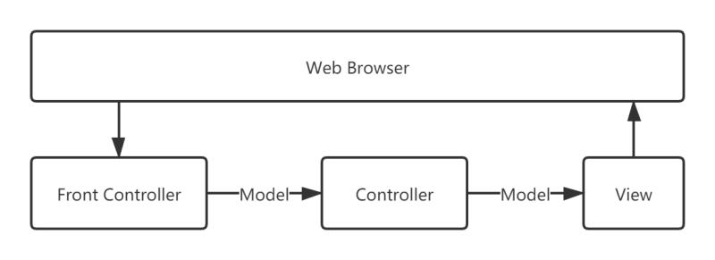
\includegraphics[width=5in]{FIGs/chapter2/springMVC.pdf}
    \caption{Spring MVC框架图}\label{fig_springMVCCH2}
\end{figure}
\begin{itemize}
  \item 前端控制器(Front Controller):DispatcherServlet类在Spring Web MVC中用作前端控制器,主要负责管理Spring MVC应用程序的流程。
  \item 模型(Model):应用程序的数据(单个对象或对象的集合)。
  \item 控制器(Controller):应用程序的业务逻辑。使用@Controller批注将类标记为控制器。
  \item 视图(View):以特定格式表示所提供的信息。通常,JSP和JSTL用于创建视图页面。尽管Spring还支持其他视图技术,例如Apache Velocity,Thymeleaf和FreeMarker~\cite{xf2012}。
\end{itemize}
\begin{figure}[htbp!]
    \centering
    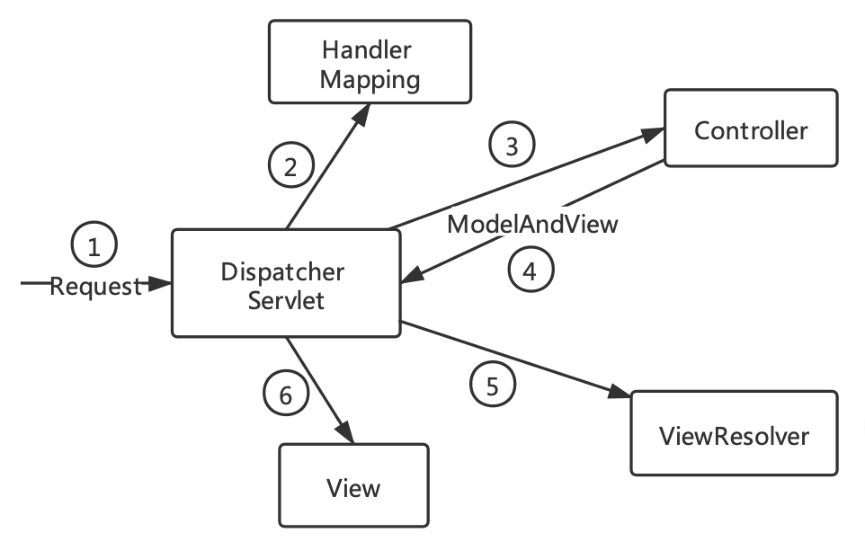
\includegraphics[width=5in]{FIGs/chapter2/springMVC2.pdf}
    \caption{Spring MVC流程图}\label{fig_springMVC2CH2}
\end{figure}

如图~\ref{fig_springMVC2CH2}所示是Spring MVC的流程图,所有传入的请求都被作为前端控制器的DispatcherServlet拦截。DispatcherServlet从XML文件获取HandlerMapping映射的条目,并将请求转发给Controller。Controller调用相关业务逻辑返回ModelAndView的对象,随后DispatcherServlet检查XML文件中视图解析器ViewResolver的条目,并调用指定的视图组件。
Spring MVC的优点:
\begin{itemize}
    \item 角色分离:Spring MVC分离每个角色,其中模型对象(model object)、控制器(controller)、命令对象(command object)、视图解析器(view resolver)、DispatcherServlet、验证器(validator)等可以由特定的对象来实现~\cite{ab2006}。
    \item 轻量级:使用轻量级Servlet容器来开发、部署应用程序。
    \item 配置强大:为框架和应用程序类提供了可靠配置,包括可以跨上下文的轻松引用,例如从Web控制器到业务对象和验证器。
    \item 快速开发:Spring MVC促进了快速并行开发。
    \item 业务代码可重用:可以使用现有的业务对象,无需创建新对象。
    \item 易于测试:在Spring中,通常创建JavaBeans类,可使用Setter方法注入测试数据。
    \item 映射灵活:提供了可轻松重定向页面的特定注释。
\end{itemize}

\section{Spring Cloud微服务部署架构}
传统软件项目一般采用的都是单块架构,对于一个逻辑上会分为多层的系统,它会把经历开发、编译、测试、打包、部署后的代码运行到同一个进程内,不断扩大的业务规模和不断变更的业务逻辑会将单块架构的劣势愈演愈烈~\cite{ln2019}。不光是激增的模块、代码会使得项目变得冗余复杂,降低代码的灵活性、易用性和可维护性,各个功能模块往往也会依赖相同或是相关的内存、数据库等内容,如果某个资源模块出错有可能导致整个系统崩溃。

Spring Cloud微服务部署架构是一系列框架、组件的有序集合,它与Spring Boot相结合,大大降低了分布式系统对于日常开发的复杂度。它包括一连串功能完善的微服务组件,比如智能路由和服务发现、服务跟踪、消息总线、服务容错、断路器、负载均衡、服务配置等~\cite{hqw2019}。基于其各组件的完整架构图如下图
~\ref{fig_springCloudCH2}所示:
\begin{figure}[htbp!]
    \centering
    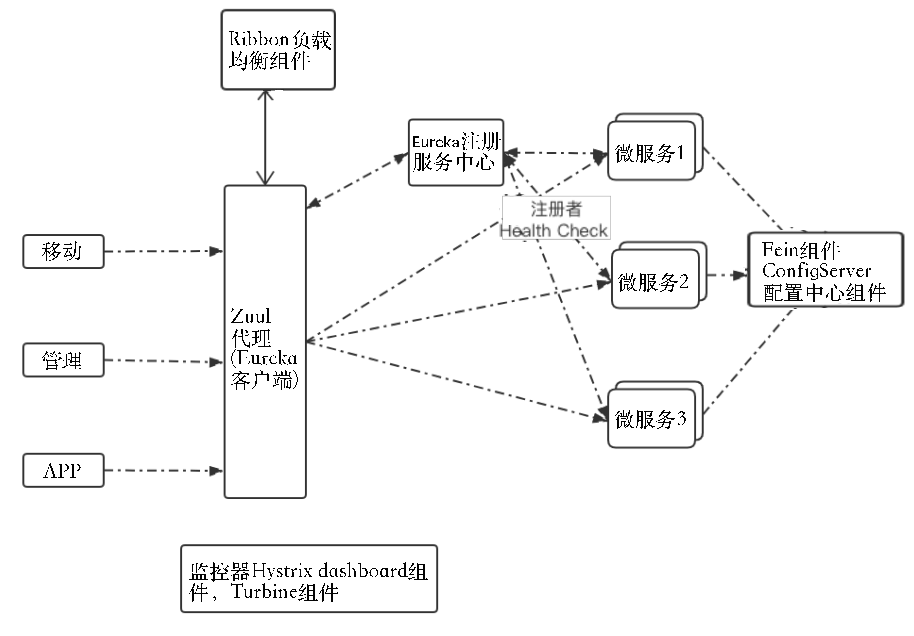
\includegraphics[width=5in]{FIGs/chapter2/springCloud.pdf}
    \caption{Spring Cloud架构图}\label{fig_springCloudCH2}
\end{figure}

Spring Cloud是一个框架,提供了在应用程序中使用云服务的工具。 当它与Eureka一起使用时,可以用作容器编排工具(提供用于大规模集成和管理容器的企业级框架的框架)~\cite{mys}。它为开发人员进行开发和部署微服务提供了友好的环境。其优点有:基于云原生的开发;基于微服务的架构;服务间通讯;遵循Spring Boot模型;与云无关。

\section{Spring Boot技术}
Spring Boot是一个Spring模块,向Spring框架提供RAD(快速应用程序开发)功能。它是一个在Spring框架顶部构建的项目,提供了一种简单、快速的方法来设置、配置和运行基于Web的应用程序。它简化了Spring的应用开发过程,节省了开发人员的时间,其核心思维是约定优于配置,尽量使其自发完成,简化系统开发。

如图
~\ref{fig_springBootCH2}
所示,Spring Boot是Spring框架(Spring Framework)和嵌入式服务器(Embedded Servers)的结合。在Spring Boot中,不需要XML配置(部署描述符)。它使用约定而不是配置软件设计范例,这意味着它减少了开发人员的工作量。
\begin{figure}[htbp!]
    \centering
    \includegraphics[width=5in]{FIGs/chapter2/springBoot.pdf}
    \caption{Spring Boot组成图}\label{fig_springBootCH2}
\end{figure}

Spring Boot使用了依赖注入方法,包含了强大的数据库事务管理功能,简化了与其他Java框架(如JPA/Hibernate ORM、Struts等)的集成,减少了应用程序的成本和开发时间~\cite{gblSpringBoot}。

Spring Boot的优点有很多:
\begin{itemize}
    \item 它创建可以使用Java -jar启动的独立Spring应用程序。
    \item 借助Tomcat、Jetty等不同的嵌入式HTTP服务器,可以轻松调试Web应用程序。
    \item 不需要部署WAR文件,能直接嵌入Tomcat中。
    \item 提供了自动配置的“starter”POMs(项目对象模型),来简化Maven配置。
    \item 提供了可用于生产的功能,例如指标、运行状况检查和外部化配置。
    \item 不需要XML配置。
    \item 提供了CLI工具,用于开发和测试Spring Boot应用程序。
    \item 提供了许多插件。
    \item 最大程度地减少了编写多个模板代码(该代码在几乎没有任何更改的情况下包含在许多地方)、XML配置和注释。
\end{itemize}

\section{Druid数据库连接池}
Druid是一个高效的开源数据库连接池,可以聚合查找大量基于时序的数据,这里基于时序是指数据的实时性,从数据库实时获取数据放入Druid后,外部系统就可以立刻查到。

\begin{figure}[htbp!]
    \centering
    \includegraphics[width=5in]{FIGs/chapter2/druid.pdf}
    \caption{Druid工作流程图}\label{fig_druidCH2}
\end{figure}
如图
~\ref{fig_druidCH2}
官方提供的Druid工作流程图所示,Druid是由多种节点组成的分布式系统,每个节点按照职责划分成不同角色,包括如下五种类型。

\begin{itemize}
    \item Historical:这类节点用于存储和查询历史数据,需要从Deep Storage获取Segment,还需要响应Broker对于Segment的查询请求。此外,Historical还需要向Zookeeper声明自己的存在.
    \item Coordinator:这类节点用于检测Historical节点中数据的可用和冗余,通过Zookeeper来发现Historical节点。
    \item Broker:这类节点用于接收外部调用方的查询请求,然后转发到Historical和Realtime,并且还需要把结果Merge之后再返回给调用者,同样通过Zookeeper感知Historical和Realtime。
    \item Indexing Service:主要用于从Realtime获取实时数据或批量插入数据。
    \item Realtime:主要用于从数据库获取实时数据。
\end{itemize}

除了上述五种节点外,Druid还有三个外部依赖:用于管理各个Druid节点的Zookeeper集群;数据库存储实例,如MySQL等;用来做Deep Storage的HDFS。

\section{Redis}
Redis是一个完全开源免费的非关系型数据库(NoSQL),项目由VMWare赞助开发。它使用高效的C语言开发,基于键值对存储,支持网络交互,数据可以存储在内存也可以持久化存储~\cite{zch2017}。在Redis中,Value支持如下几种数据类型:

\begin{itemize}
    \item String:字符串,是Redis中最基本的数据类型,也是任何存储系统都必备的数据类型。
    \item List:字符串列表,其中的数据是有序并允许重复的,底层实现是链表而不是数组。数据按照插入顺序排序,也可以在列表的头部、尾部或任意位置插入数据。
    \item Set:字符串集合,其中的数据是无序并且不允许重复的。基于哈希表实现,插入、删除、查找三种操作的时间复杂度均为常数级,效率较高。
    \item 	Sorted Set:有序字符串集合,基于Set之上添加了有序性,实现方法是为每个元素关联了一个浮点数类型的值,基于这个值来做数据的排序。
    \item Hash:键值对哈希表,其中Key和Value都是String类型的,是从redis-2.0.0版本之后才支持的数据类型。
\end{itemize}

由于对内存中数据的读写速度远高于磁盘读写,因此Redis作为缓存使用时主要使用内存存储数据~\cite{wyl2019}。但Redis同样也支持数据持久化,主要有两种方式,分别是RDB(Redis DataBase)和AOF(Append Only File),两种方式可以同时使用。RDB简单来讲就是对Redis的内存数据生成一份快照并存储到磁盘等存储介质中,AOF则是将Redis执行过的所有写指令记录下来,数据恢复时只需要把这些指令按顺序执行即可。

此外,Redis具有原子性,即Redis的所有操作都是原子性的,执行结果只有成功和失败两种可能,同时也支持多个操作的事务管理~\cite{xmh2019}。这里的事务跟一般的数据库事务一样,是一种隔离操作,用于一次性按顺序执行多个指令。Redis事务同样具备原子性,如果Redis在某个事务执行过程中崩溃退出,导致该事务只执行了部分命令,那么Redis重启时会自动检测并移除部分执行的事务~\cite{wzf}。

\section{前端技术}
该系统的前端开发主要使用React、Redux,其中React具有组件化开发、单项数据流的特性,使得其具有良好的灵活性、组件性、流动性、和隔离性,将一个页面划分成多组件进行开发,以此来独立开发功能之间相互独立的组件,并可以重复使用。同时使用了Immutable.js创建数据,减少系统内存消耗,界面的各类组件设计使用了蚂蚁金融开发的Ant Design设计体系的React UI组件库——antd,进行快速、美观、高效的前端界面开发。\\

\subsection{React和Redux}
React是一个声明式、组件化、高效灵活的用于构建UI用户界面的开源JavaScript库。使用React将创建交互式UI变得简单,为应用中的各类状态设计了简明视图,使得React能在数据发生变化时进行有效更新以及渲染组件,将代码变得可靠、清晰、方便调试。它创建了拥有独立状态的不同组件,再将这些简洁且独立的组件组合构成较为复杂的UI界面。

React组件可以接收各类数据使用render()方法进行界面渲染,通常存储为JSX类文件,被传入的外部数据通过this.props可以在组件内访问,此外组件还可以维护内部数据,通过this.state访问,通过this.setState()方法来更新,当组件内部数据发生改变时,组件会调用render()方法进行对应标记部分的重新渲染~\cite{yxq}。

React有很多优点,它的组件化、模块化使得代码的复用性、可维护性非常高,使用虚拟DOM操作既解决了跨浏览器问题,提供了标准化API,又加快了渲染速度,提升Web性能,有序的单项数据流方便进行开发管理\cite{lh}。然而,多个数据层与多个组件交互构成数据流时,随着数据规模的不断扩大,一些反响数据流就会变得十分复杂,从而产生许多无法估量的问题。这里引用了Redux,它是由Flux演变而来的,没有Flux的复杂性,变得简单、易上手,是JavaScript的状态容器,使得状态管理变得可预测。

Redux具有三大特性:
\begin{itemize}
    \item 单一数据源:应用中的所有State都储存在一棵Object Tree中,且Object Tree只会在唯一的Store中存在。这就使得开发和调试变得简单,比较复杂的功能,例如撤销、重做也变得非常容易。
    \item State是只读的:改变State的方法只有一种——触发Action。Action是用来描述已经发生了的事件的一个普通对象,可以被序列化、存储、后期调试、日志打印或者测试时被回放。这样一来可以保证网络请求和界面视图都不可以直接修改State状态,如果想要修改则只能表达要修改的意图,然后由Redux集中处理,并且按照顺序逐个执行,不会出现竞态条件(Race Condition)。
    \item 使用纯函数执行修改:需要通过撰写Reducer来描述Action是如何改变State Tree状态树的。Reducer用于接收之前的State和Action,依次返回新的State,它是纯函数。用户可以编写很多可以独立操作State Tree不同功能部分的Reducer,控制其调用顺序、传入一些数据参数,也可以编写一些可复用的Reducer用于处理比如分页器等的通用任务。\\
\end{itemize}

\subsection{Immutable.js}
Immutable通俗来讲就是一个可以实现数据结构持久化的JavaScript库,它是一系列一经创建不能被改变的数据结构的集合,可以和Rudex对接良好。系统主要使用的几个持久化数据结构有:Set、List、Map,可以高效链接map、filter等方法。数据一旦创建无法更改,Immutable提供了一个可变API来产生新的更新数据,不去更新原有数据。这样可以简化应用程序的开发过程、减少内存消耗、使用简单的逻辑实现检测更新技术。\\

\subsection{antd}
antd是基于蚂蚁金融开发的Ant Design设计体系的一套React UI组件库,主要用于研发、设计企业级中后台的产品UI界面。它的出现可以提炼产品的视觉风格、交互语言,是开箱即用的质量比较高的React组件,与本系统的前端框架刚好吻合,支持多种语言、可以进行个性化主题定制,安装简单且容易上手。减少了人工设计基础组件的时间、成本浪费,可以有效提高系统的界面美观度和开发效率。\\

\subsection{React-AMap}
React-AMap是React封装的高德地图组件,可以比较简单、快速地将地图接入到项目中。本系统H5界面的外卖点单中用户地址的选择和Web界面的座位库平面视图均使用了该技术,主要用到的组件有Map、Marker,由于需求比较复杂、个性化,系统还根据高德地图原生的API自定义了组件MouseToolPlugin进行地图上图标的管理。

React-AMap组件拥有的属性,分为基本类型值和引用类型值,比如Map的属性zoom属于数字类型值,属性center属于引用类型值。定义React-AMap的引用类型属性,最好在React生命周期中的constructor和componentWillMount方法中实现,可以在组件中进行引用\cite{hhl2011}。在组件中,可以通过props访问到高德地图实例和其中的div容器类型,进而可以自定义地图组件和功能。React-AMap组件有一些已经存在的扩展组件,比如热力图组件(react-amap-plugin-heatmap)、定位组件(react-amap-plugin-geolocation)、可定义的AMapUI组件(react-amapui-wrapper)。\\

\subsection{Webpack}
Webpack一般用于前端的打包,它是一个JavaScript(JS)应用程序的高度可配置的静态模块打包工具,它通过递归构建包含应用开发程序所需要的各个模块的依赖关系图,接着将其打包成相应数量的bundle。主要包括四个核心概念:entry、output、loader和plugins。其中entry用于指示使用哪个模块开始构建内部的依赖图,当找出入口起点直接和间接依赖的库或者模块时,将依赖处理并输出到bundles内,默认值是./src。output用于指定输出bundles的位置、如何命名,编译整个的程序结构到指定的输出路径文件夹,其默认值是./dist。由于Webpack本身只能理解JS,这就需要loader处理一些非JS文件,将其处理成Webpack可以进行打包的有效模块。打包优化、代码压缩、分离、去重、重新定义环境变量等内容都在plugins插件范围内,它依靠插件的接口功能可以处理很多复杂任务。

\section{Kafka消息系统}
Kafka是一个基于Zookeeper协调的分布式发布订阅消息系统,它支持分区、多副本、异步处理、高吞吐量、持久可靠、可扩展、负载均衡、容错性高、高并发,可以实时处理海量数据从而满足系统所需的各种场景。主要是由Scala语言和Java语言编写,使用场景很多,可以用于收集各种服务log日志;跟踪用户活动,做一些监控、离线分析、挖掘;高解耦可用作消息系统;收集数据并生产各种操作的反馈,记录运营监控数据,用于运营指标;可以进行一些比如Spark Steaming等的流式处理;事件源\cite{lb2019kafka}。

Kafka具有四个比较核心的API:
\begin{itemize}
    \item Producer API可以让应用程序的记录流发布到若干个Kafka主题。
    \item Consumer API可以让应用程序订阅若干Kafka主题,处理生成的记录流。
    \item Streams API可以让应用程序作为流处理器,使用若干主题的输入流来生成若干输出主题的输出流,从而有效可靠地把输入流转换成为输出流。
    \item Connector API可以构建、运行可重用生产者或者使用者,它们将Kafka主题链接到已有的应用程序、数据系统。
\end{itemize}

\section{微信支付宝支付}
\subsection{微信支付}
微信支付参照其开发文档,支付模式一共有六种,分别是付款码支付、Native支付、JSAPI支付、APP支付、H5支付、小程序支付。本系统是嵌入在微信、浏览器中的H5界面和Web界面,用到了以下三种支付模式:
\begin{itemize}
    \item Native支付:系统的Web网页端按照微信给的支付协议生成商家的支付二维码,用户打开微信“扫一扫”,扫码完成支付。该模式适用场景有:PC端网站支付、实体商店单品支付、订单扫码支付、媒体支付、广告支付等。
    \item JSAPI支付:用户在微信中打开商家的H5页面,本系统的H5界面嵌入在微信公众号内,商家在该页面通过后端调用微信支付所提供的JSAPI支付接口,回调微信支付模块以此完成支付功能。该模式适用场景有:用户从微信点击进入商家公众号,从某商家主页完成支付;用户在聊天界面、朋友圈等点击商家链接,打开页面完成支付;用户扫描由商家页面转换成的二维码,从微信浏览器中进入该商家页面进行支付操作。
    \item 	H5支付:用手机、平板等移动设备通过浏览器进入商家页面,唤起微信支付进行支付。
\end{itemize}

本系统的顾客点单平台中,嵌入在微信公众号内的H5界面,需要在微信平台内进行支付,支付方式只能用微信支付。
首先需要登录公众号进行JS接口安全域名的填写,并获取openid,它是商家在微信公众号appid下的唯一用户标识(与appid一一对应),可以永久标记用户,也是使用JSAPI支付必须要传的一个参数。
用户新建一个授权url页面,当授权成功会根据用户设定的(redirect uri)重定向地址
跳转到相应地址,并得到授权返回的code,将该code码作为参数调用后端接口,返回openid。
在微信公众号内,需要添加支付页面的地址,并将其作为参数调用后端接口,返回值可以配置wx.config。获得返回值后,再通过wx.ready调用wx.chooseWXPay进行微信支付即可支付成功。\\

\subsection{支付宝支付}
支付宝的支付功能比微信支付简单一些,它只能在非微信平台内调用。支付宝支付需要有支付宝开放平台的账号,在该网站内创建一个应用,填写相关信息,审核通过后即可配置沙箱环境。由于支付涉及到金钱安全问题,支付宝提供了一种模拟支付环境——蚂蚁沙箱环境,用来帮助开发者对功能接口进行开发和联调。

\section{本章小结}
本章主要从定义、工作原理、架构、特性等几个方面,介绍了彭庆福餐厅点单系统开发过程中用到的相关开发框架和技术。整个系统采用Spring Cloud微服务部署架构进行搭建,与Web服务相关的接口按照REST风格进行设计。其中,后端技术使用了Spring MVC、Spring Boot,数据库用到了MySQL、Druid、Redis,前端技术使用了antd、React、Redux、微信支付宝支付以及高德地图组件React-AMap、Immutable、Webpack,还介绍了Kafka消息系统。


\chapter{彭庆福餐厅点单系统需求分析与概要设计}
本章对彭庆福餐厅点单系统进行了需求分析和概要设计,描述了系统设计目标、功能需求和非功能需求。介绍了系统总体设计与部署,通过数据库实体关系图解释了数据库设计。

\section{系统需求概述与可行性分析}
\subsection{系统设计目标}
彭庆福餐厅点单系统的核心目标是解决用户到店点餐、预约点餐、外卖点餐、付款、帮助与反馈等问题,同时为商家提供座位管理、菜品录入、库存预警、统计报表等功能。

本系统应该具有以下几个核心目标:
\begin{enumerate}
  \item 实现高效在线点单:系统提供到店、预约、外卖形式的点餐服务为顾客充分提供便利,节省排队点餐、等待上菜等时间,并为顾客自动保存购物车内已点菜品,保存外卖、预约点单的历史内容。
  \item 支持多角色点单:同一个顾客可能会有不同身份来用餐,比如工作时可以使用公司角色并享受相应的订单折扣,日常就餐可以使用个人角色,所以系统设置了多角色切换,允许用户使用所选角色进行点单。
  \item 到店用餐时,订单和座号相关联:顾客到店点餐时,将订单与座号绑定,顾客可以下单、加菜、取消订单、支付订单,只有当订单结束时,此座位才会转为开放状态,可以供下一位顾客使用。
  \item 实现在线支付结账:顾客不需要再去收银台结账,可以自行下单并且用支付宝、微信等方式支付订单。
  \item 较高问题解决率:系统有帮助与反馈入口,顾客可以提出意见与建议,系统会检索有无相关问题答案,如果有相关问题的答案,系统会快速反馈给顾客,如果没有,系统会发送给商家并在得到解答后返回给用户。
  \item 实现菜品信息录入:商家可以将菜品录入到每日要出品的发布中,使得顾客下单的时候可以及时看到当日菜品图片、名称以及其价格、份数等详情。
  \item 实现座位管理:商家可以录入餐厅位置实地信息,并登记座位,实时管理座位数、状态、是否拼单等信息。
  \item 实现库存管理:商家在采购需求中可以快速登记,录入当日所缺菜品,并且在生产实况中可以看到当前菜品空缺详情。
  \item 符合用户使用软件的习惯:顾客想点餐的时候需要方便快捷的渠道,而商家接单、处理订单一般在固定地点办公,所以系统将点单部分和管理部分分别设计成了包括微信公众号、支付宝和网页浏览在内的移动端和PC端,使得用户习惯该系统的使用方式。
\end{enumerate}

如图
~\ref{fig_strucCH3}所示,整个彭庆福餐厅点单系统由移动端、PC管理平台及后台服务器组成,顾客可以使用微信公众号、微信扫一扫、支付宝扫一扫或者Safari、IE、Chrome等浏览器以H5网页的形式接入到该系统,商家可以使用电脑以基于B/S模式的PC端网页的形式接入系统来管理菜品、订单等,后台服务器则为前端提供所需的各种接口服务~\cite{yamamoto1999raw}。
\begin{figure}[htbp!]
    \centering
    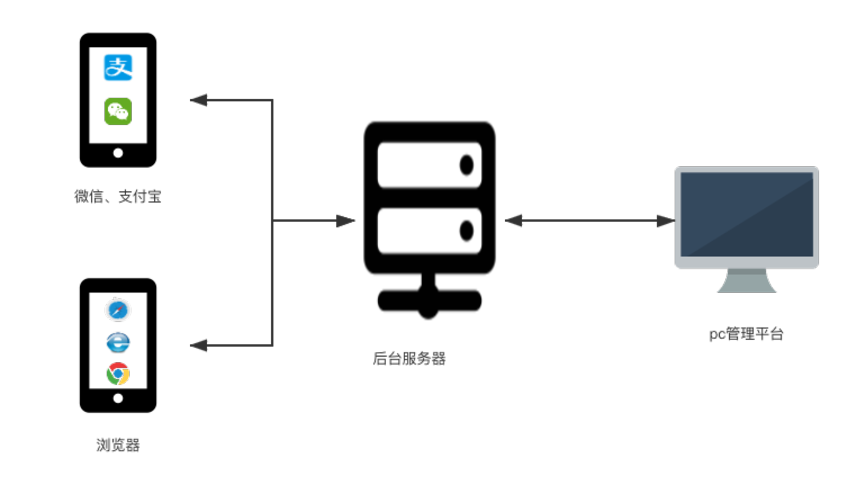
\includegraphics[width=5in]{FIGs/chapter3/struc.pdf}
    \caption{系统整体结构图}\label{fig_strucCH3}
\end{figure}

\subsection{需求概述}
为了满足顾客点餐时对于隐私的要求以及商家对点餐系统菜品溯源、订单管理与座位管理上的要求,本文设计了彭庆福餐厅点单系统,该系统从顾客和商家两方考虑,充分满足了二者对点单、管理上的需求,商家记录餐厅、菜品、座位、订单等信息,便于顾客查看餐厅详情、订单历史数据以及个人信息。
\begin{figure}[htbp!]
    \centering
    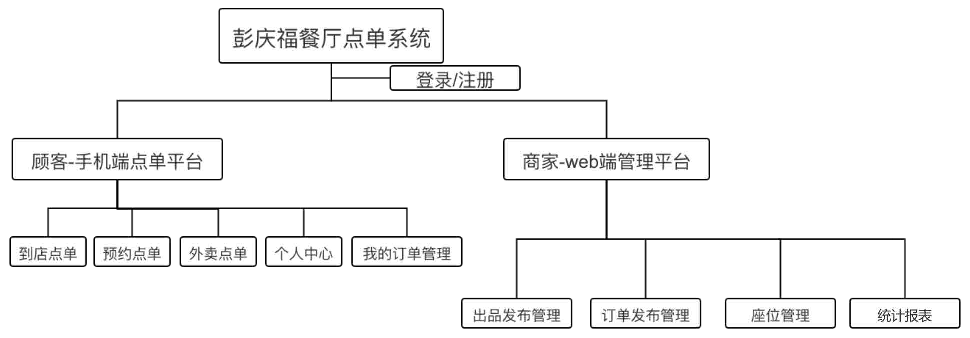
\includegraphics[width=5in]{FIGs/chapter3/function.pdf}
    \caption{系统功能需求结构图}\label{fig_functionCH3}
\end{figure}

如图
~\ref{fig_functionCH3}所示,彭庆福餐厅点单系统的入口有两种,一种是移动端包括浏览器、微信公众号以及支付宝扫码,需要实现顾客点单、支付、查看订单、修改个人信息;另一种是Web网页端,商家进行出品发布管理、订单发布管理、座位管理、菜品管理、统计报表等多种功能需求。

其中,顾客可以通过到店扫码、关注微信公众号、浏览器直接输入地址等方式进入平台,登录注册后实现到店、预约、外卖点单等操作。商家可以通过Web地址从电脑网站直接进入平台进行管理,实现从注册商家到登记菜品、创建座位仓库、创建出品发布、管理订单发布、管理座位信息、管理菜品等操作。\\

\subsection{可行性分析}
技术可行性:后端采用Spring Cloud微服务部署架构与Spring Boot技术的结合,这类开发技术已经比较完善、成熟,可供参考的技术资料比较充足,可以对接分布式发布订阅消息系统Kafka进行数据流方面的处理。前端采用的React与Redux框架比较稳定且易上手,UI方面使用蚂蚁金服设计的比较成熟的Ant Design达到视觉上美观、统一的效果。因此,本系统的可行性非常高。

经济可行性:随着国民经济的不断提升以及互联网的飞速发展,人们对于饮食方面的需求越来越多样化,对隐私的要求也越来越高,传统的点单系统已经无法满足多样化需求,急需一款可以保护用户隐私,帮助顾客推荐喜好、查看历史操作、查看菜品原料从采摘到售卖的历史记录,帮助商家进行库存管理、报表分析、订单管理等操作的新型点单系统。彭庆福餐厅点单系统为实现这些需求应运而生,具有良好的发展前景。该系统上手难度小,参考代码模板多,并且已经与餐厅提前沟通好宣传方案,其开发成本、推广成本都比较低,具有比较高的经济效益前景。

\section{系统需求分析}
\begin{table}[htbp!]\footnotesize
  \centering
  \caption{彭庆福餐厅点单系统的主要功能需求列表}
  \vspace{2mm}
  \begin{tabular}{clp{0.6\columnwidth}}
  \toprule
  \textbf{需求编号}&\textbf{需求名称}&\textbf{需求描述}\\
  \midrule 
  \textbf{R1}& 到店点单& 顾客到店后,扫描桌子上二维码点单就餐,可以在线选购菜品、加菜、退菜、取消订单、付款。\\
  \hline
  \textbf{R2}& 预约点单& 若餐厅未在营业时间内,顾客可以手机预约点单,填写用餐时间、人数、电话后,在线预约下单,并在该时间段去店内就餐。\\
  \hline
  \textbf{R3}& 外卖点单& 顾客可以随时随地在手机上进行外卖点单,填写收货地址、配送时间、联系姓名、联系电话以及人数后,在线下单外卖等待配送。\\
  \hline
  \textbf{R4}& 个人中心& 顾客可以在个人中心查看个人状态、更改角色、退出登录,在帮助与反馈栏中提出意见等。\\
  \hline
  \textbf{R5}& 我的订单管理& 顾客可以打开我的订单,查看订单列表,可点击具体订单查看订单详情、支付订单,可以对未完成订单进行退菜、加菜、取消订单等操作。\\
  \hline
  \textbf{R6}& 出品发布管理& 商家可以每日创建一个出品发布,来设置当天餐厅营业时间段、菜品管理(包括菜品类别管理、增删改菜品)、查看采购需求、进行菜品的快速登记。\\
  \hline
  \textbf{R7}& 订单发布管理& 当顾客手机下单后,商家可以查看到当前餐厅的所有订单列表,可对订单进行删改,点击进入相应订单查看详情,进行取消菜品、结算、确认顾客离店、打印订单等操作。\\
  \hline
  \textbf{R8}& 座位管理& 商家可以设置餐厅开放时间,多视图(卡片视图、平面视图、时间轴视图)管理座位仓库,座位设置成功后会有和每个座位相对应的二维码,可以对座位及二维码信息进行管理。\\
  \hline
  \textbf{R9}& 统计报表& 商家点击报表查看每日、每月的收支报表、菜品进销存报表,可以根据时间筛选查看或打印任意日期的报表内容。\\
  \bottomrule
  \end{tabular}
  \label{table:requireList}
\end{table}

该系统涉众主要两种,分别是顾客和商家。不同的用户角色对于该系统有如下需求:

\begin{enumerate}
    \item 顾客:顾客随时随地都有可能点单,并且在系统使用过程中可能会遇到一系列自己无法解决的问题,他们需要一个方便、快捷的平台,可以快速而准确地满足其饮食需求。最佳方式就是注册并登录该系统,将所需菜品直接选购下单完成付款。
    \item 商家:商家一般是熟悉餐厅运营,了解菜品详情、每日库存与订单详情的员工,对菜品销售非常熟悉并且有固定的办公场地。他们需要一个系统来统计菜品销售和库存,处理顾客的各种订单与问题,录入当日菜品数量、更新库存等。
  \end{enumerate}

通过以上分析可以得出如表~\ref{table:requireList}所示的彭庆福餐厅点单系统的部分主要功能需求,以下分别从顾客和商家角度对该系统功能需求作出具体分析。\\

\subsection{顾客功能需求}
顾客功能需求部分是彭庆福餐厅点单系统中主要由手机操作的部分,其用例图如图
~\ref{fig_customerCH3}所示,主要包括了到店点单、预约点单、外卖点单、个人中心、我的订单管理等功能,其具体包含功能如下:
\begin{figure}[htbp!]
  \centering
  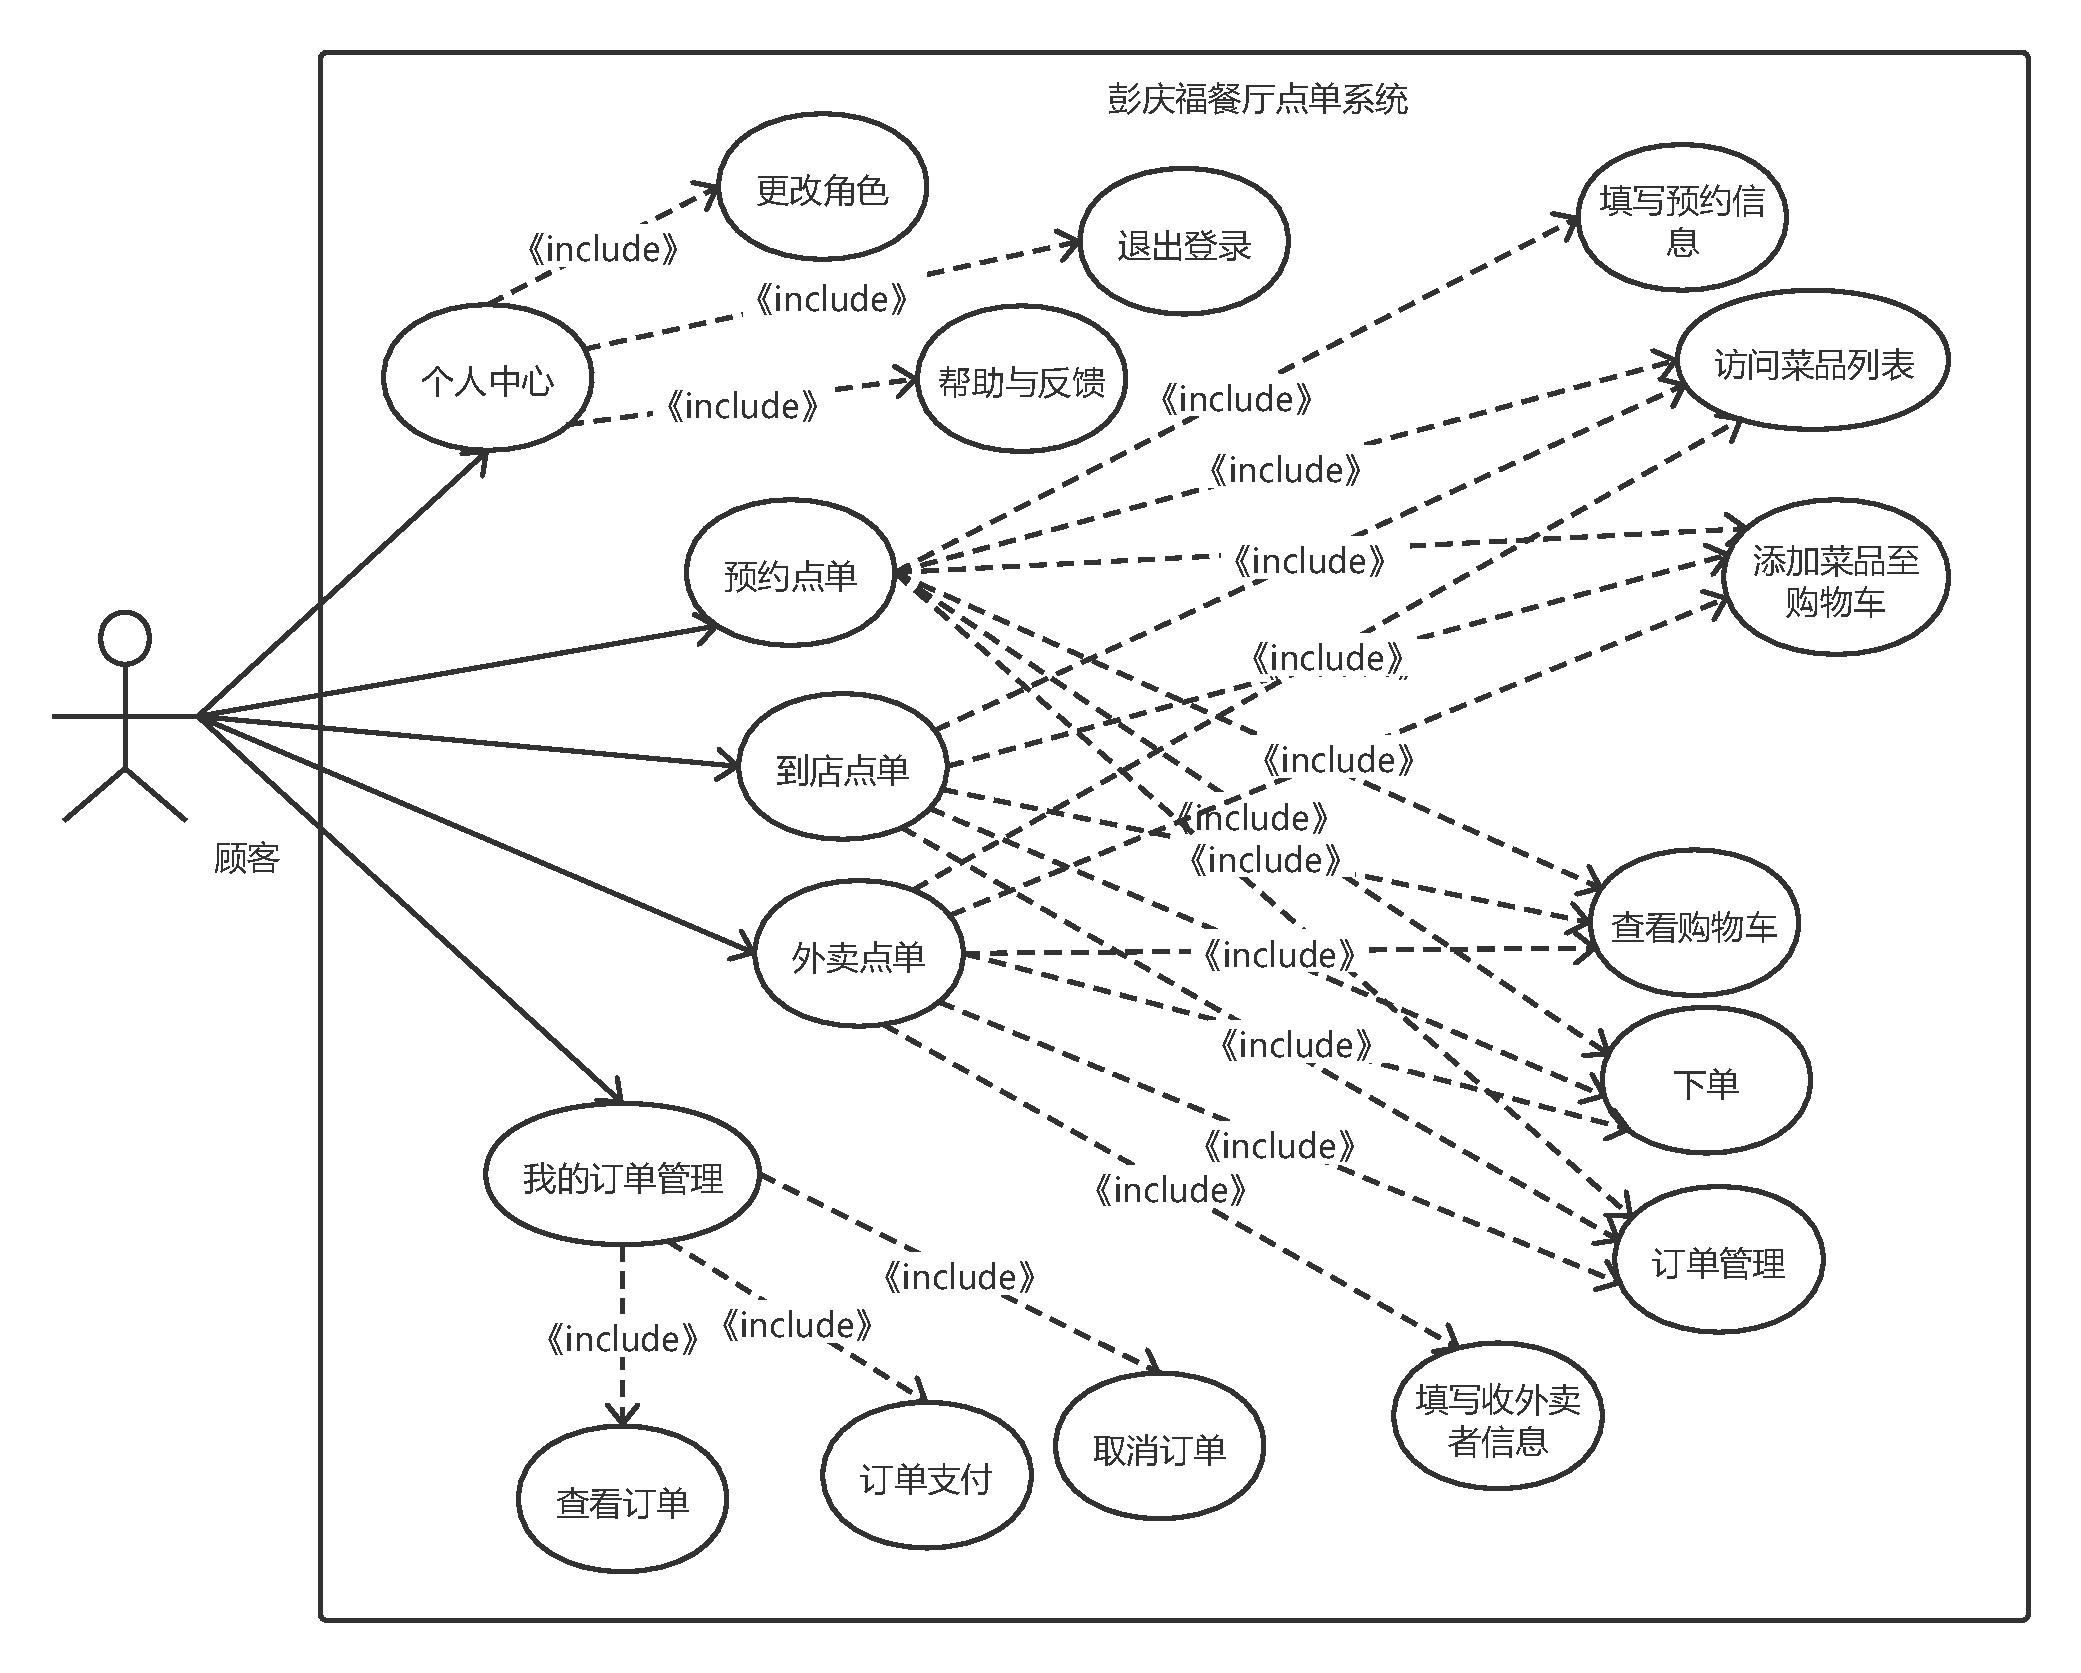
\includegraphics[width=5in]{FIGs/chapter3/customer.pdf}
  \caption{顾客就餐模块用例图}\label{fig_customerCH3}
\end{figure}

下面将详细描述关于顾客点单平台的几个重要用例。

如表~\ref{table:uc1}所示,其描述了顾客到店点单的具体过程,顾客在成功登录系统后点击店内就餐可以选定座位并扫描桌上二维码进行点菜、增删所选菜品数量、查看购物车、下单等操作。用户到店点单时,需要扫描座位上的二维码才能进行下单,如果该座位当前已经有订单,系统会提醒顾客,并且判断座位的当前订单是否为该用户订单,如果是则提示跳转到该订单详情页,如果不是则提醒用户该座位已有订单,需要换一个座位下单。

顾客预约点单与之类似,未在餐厅营业时间时或者想要提前预约之后时间来就餐,顾客可以选择提前预约点菜下单,在指定时间就餐或者在此之前取消菜品即可。系统考虑到顾客隐私安全问题,在账号登录时需要用户认证,付款时也需要二次认证保护顾客付款的安全性。顾客将部分菜品加入购物车后,不小心退出点单界面,之后再次进入时,系统会记录顾客历史操作,保留购物车内菜品,方便顾客继续点单。

\begin{table}[htbp!]
  \footnotesize
  \centering
  \caption{到店点单用例表}
  \vspace{2mm}
  \begin{tabular}{cp{11.5cm}}
   \hline
   \ ID & UC1 \\ 
   \hline
   \ 名称 & 到店点单 \\ 
   \hline
   \ 参与者 & 顾客,目标是根据个人需要创建一个菜品订单。 \\ 
   \hline
   \ 优先级 & 高 \\ 
   \hline
   \ 触发条件 & 用户需要在餐厅内用餐。 \\ 
   \hline
   \ 前置条件 & 用户成功登录彭庆福餐厅点单系统,并拥有点单权限。 \\ 
   \hline
   \ 后置条件 & 菜品订单创建成功,用户成功用餐。 \\ 
   \hline
   \multirow{2}{*}{正常流程}
    & 1.	已成功登录的用户进入主页,点击店内就餐。\\
    & 2.	系统按照不同类别显示该餐厅当日所有菜品。\\
    & 3.	用户扫描座位上二维码。\\
    & 4.	系统显示相应座位号。\\
    & 5.	用户选择就餐角色、就餐时间、就餐人数以及菜品种类和数量,点击下单。\\
    & 6.	系统提示下单成功,并展示订单详情。\\
    & 7.	用户查看详情并选择相应操作。\\
    & 8.  系统保存用户修改并更新界面。 \\
   \hline
   \multirow{2}{*}{扩展流程}
    & 3a. 未在商家营业时间:\\
    & ~~1.	系统提示未在营业时间,接受预约,用户无需扫码。\\
    & ~~2.	返回步骤5。\\
    & 3b. 该用户当前有未完成的到店订单:\\
    & ~~1.	系统提示用户还有未完成订单,并跳转到相应订单详情页面。\\
    & 3c. 该座位当前有未完成的订单,且不是该用户的:\\
    & ~~1.	系统提示用户该座位已有订单,提示其更换座位下单。\\
    & ~~2.	返回步骤2。\\
    & 7a. 用户选择加菜:\\
    & ~~1.	系统返回菜单页面供用户添加菜品并下单。\\
    & 7b. 用户选择相应菜品退菜:\\
    & ~~1.	系统保存更改并更新订单详情页面(退掉的菜品不会再显示)。\\
    & 7c. 用户选择取消订单:\\
    & ~~1.  系统保存更改并更新订单详情页面(订单状态变成已取消)。\\
  \hline
  \ 特殊需求 & 无 \\ 
  \hline
  \end{tabular}
  \label{table:uc1}
\end{table}

如下表~\ref{table:uc2}所示,其描述了顾客外卖点单的具体过程,顾客在成功登录系统后点击外卖点餐可以选择地址,填写收外卖者信息,进行点菜、增删所选菜品及修改其数量、查看购物车、下单等操作。顾客可以在操作的任意步骤内返回上一页面进行内容修改,系统会保存顾客操作,提高可用性。由于到店点单、预约点单与座位相关联,所以一个用户同一时刻只能有一个正在进行的相关订单,但是外卖订单可以同时下单多个,根据顾客需要送至相同或不同地址。

此操作可以帮助顾客随时随地点单,系统会默认记录收外卖者信息,使得下次点单时不需要再重新录入个人信息。外卖点单的选择地址组件引用了高德地图API的React组件——React-AMap,不光自动定位当前位置,顾客还可以自由定位所在位置或者搜索选定某一位置作为接收地点,系统会判断外卖是否在商家配送范围内并进行相应提醒。在商家确认订单之前,顾客可以选择取消订单,并且可以随时查看订单状态,跟踪骑手位置,有效帮助顾客了解订单详情,提升其就餐满意度。
\begin{table}[htbp!]
  \footnotesize
  \centering
  \caption{外卖点单用例表}
  \vspace{2mm}
  \begin{tabular}{cp{11.5cm}}
   \hline
   \ ID & UC3 \\ 
   \hline
   \ 名称 & 外卖点单 \\ 
   \hline
   \ 参与者 & 顾客,目标是根据个人需要创建外卖订单。 \\ 
   \hline
   \ 优先级 & 高 \\ 
   \hline
   \ 触发条件 & 用户需要外卖用餐。 \\ 
   \hline
   \ 前置条件 & 用户成功登录彭庆福餐厅点单系统,并拥有点单权限。 \\ 
   \hline
   \ 后置条件 & 外卖订单创建成功,用户成功用餐。 \\ 
   \hline
   \multirow{2}{*}{正常流程}
    & 1.	已成功登录的用户进入主页,点击外卖点餐。\\
    & 2.	系统显示需要用户填写的内容。\\
    & 3.	用户选择收货地址、配送时间,填写联系姓名、联系电话、人数。\\
    & 4.	用户填写完毕,点击确认并点餐。\\
    & 5.	系统按照不同类别显示该餐厅当日所有菜品。\\
    & 6.	用户选择菜品种类和数量,点击下单。\\
    & 7.	系统显示包括菜品种类、数量以及收外卖者信息和合计价格。\\
    & 8.	用户点击确认并选择付款方式付款。\\
    & 9.  系统提示下单成功,并展示订单详情。 \\
    & 10.	用户点击取消订单。\\
    & 11.  系统保存用户修改并更新界面,订单状态变成已取消。 \\
    & 用户可以重复步骤3-11,直至完成所有要下单的外卖内容。\\
   \hline
   \multirow{2}{*}{扩展流程}
    & 3a. 用户发现信息填写有误,选择返回:\\
    & ~~1.	返回步骤2。\\
    & 3b. 用户搜索地址相关字:\\
    & ~~1.	系统返回相关地址内容供用户选择。\\
    & 7a. 用户发现菜品选择有误,选择返回:\\
    & ~~1.	返回步骤5。\\
  \hline
  \ 特殊需求 & 无 \\ 
  \hline
  \end{tabular}
  \label{table:uc2}
\end{table}

如下表~\ref{table:uc3}所示,其描述了顾客管理个人中心的具体过程,顾客在成功登录系统后点击个人头像可以进入个人中心,该界面会显示当前所选角色、头像,以及用户账号等基本信息。顾客可以选择切换角色、提出意见与建议、退出登录等操作,并得到相应的反馈内容。

顾客在该页面下可以清晰看到个人信息,并且可以更换不同角色进行不同操作与查看。每个角色对应现实生活中的一种身份,比如个人角色、公司角色等,也会有与之对应的操作权限与折扣优惠。

顾客如果对软件或是餐厅有任何问题需要解决,都可以点击“帮助与反馈”按钮,填写问题详情点击提交,问题会很快反映给商家,待其解决会将反馈以消息形式推送给顾客供其查看。顾客也可以选择退出登录,则系统会将其安全退出,并跳转到登录注册页面。

\begin{table}[htbp!]
  \footnotesize
  \centering
  \caption{个人中心用例表}
  \vspace{2mm}
  \begin{tabular}{cp{11.5cm}}
   \hline
   \ ID & UC4 \\ 
   \hline
   \ 名称 & 个人中心 \\ 
   \hline
   \ 参与者 & 顾客,目标是查看并管理个人信息。 \\ 
   \hline
   \ 优先级 & 中 \\ 
   \hline
   \ 触发条件 & 用户需要管理个人信息。 \\ 
   \hline
   \ 前置条件 & 用户成功登录彭庆福餐厅点单系统。 \\ 
   \hline
   \ 后置条件 & 个人信息修改成功。 \\ 
   \hline
   \multirow{2}{*}{正常流程}
    & 1.	已成功登录的用户点击个人头像进入个人中心界面。\\
    & 2.	系统显示当前用户头像、账号以及当前角色。\\
    & 3.	用户查看详情并进行相应操作。\\
    & 4.	系统保存用户修改并更新界面。\\
    & 用户可以重复步骤3、4,直至完成所有要操作的内容。\\
   \hline
   \multirow{2}{*}{扩展流程}
    & 3a. 用户点击当前角色:\\
    & ~~1.	系统显示当前用户的所有角色。\\
    & ~~2.	用户选择想要切换的角色。\\
    & 3b. 用户点击帮助与反馈:\\
    & ~~1.	系统显示帮助与反馈界面。\\
    & ~~2.	用户输入问题,点击提交。\\
    & 3c. 用户点击退出登录:\\
    & ~~1.	系统退出当前账户。\\
    & ~~2.	系统跳转到登录界面。\\
  \hline
  \ 特殊需求 & 无 \\ 
  \hline
  \end{tabular}
  \label{table:uc3}
\end{table}

如下表~\ref{table:uc4}所示,其描述了顾客进行订单管理的具体过程,顾客在成功登录系统后点击我的订单可以查看所有历史订单记录,选择某一具体订单点击查看详情并进行管理~\cite{carroll2011system}。

\begin{table}[htbp!]
  \footnotesize
  \centering
  \caption{我的订单管理用例表}
  \vspace{2mm}
  \begin{tabular}{cp{11.5cm}}
   \hline
   \ ID & UC5 \\ 
   \hline
   \ 名称 & 我的订单管理 \\ 
   \hline
   \ 参与者 & 顾客,目标是查看我的订单并管理。 \\ 
   \hline
   \ 优先级 & 高 \\ 
   \hline
   \ 触发条件 & 用户需要查看我的订单。 \\ 
   \hline
   \ 前置条件 & 用户成功登录彭庆福餐厅点单系统,并拥有查看我的订单权限。 \\ 
   \hline
   \ 后置条件 & 我的订单查看完成。 \\ 
   \hline
   \multirow{2}{*}{正常流程}
    & 1.	已成功登录的用户进入主页,点击我的订单。\\
    & 2.	系统根据全部、未完成、已完成三种状态显示订单列表。\\
    & 3.	用户点击某一订单。\\
    & 4.	系统显示该订单详情。\\
    & 5.  用户查看详情并进行相应操作。\\
    & 6.  系统保存用户修改并更新界面。\\
    & 用户可以重复步骤3-6,直至完成所有要操作的规则。\\
   \hline
   \multirow{2}{*}{扩展流程}
    & 5a. 若当前订单商家还未确认,且非外卖订单:\\
    & ~~1.	用户选择加菜。\\
    & ~~2.	系统返回菜单页面供用户添加菜品并下单。\\
    & ~~3.	用户选择相应菜品退菜。\\
    & ~~4.	系统保存更改并更新订单详情页面(退掉的菜品不会再显示)。\\
    & ~~5.	用户选择取消订单。\\
    & ~~6.	系统保存更改并更新订单详情页面(订单状态变成已取消)。\\
    & ~~7.	用户选择支付。\\
    & ~~8.	系统根据当前操作环境和用户选择的付款方式显示相应付款界面。\\
    & 5b. 若当前订单商家还未确认,且订单类型是外卖:\\
    & ~~1.	用户点击取消订单。\\
    & ~~2.	系统保存用户修改并更新界面(订单状态变成已取消)。\\
    & 5c. 若当前订单已结束还未评价:\\
    & ~~1.	用户点击相应菜品进行评价,对本次用餐进行评价。\\
    & ~~2.	系统保存用户修改并更新界面(订单状态变成已评价)。\\
  \hline
  \ 特殊需求 & 无 \\ 
  \hline
  \end{tabular}
  \label{table:uc4}
\end{table}

根据顾客所选角色,会显示相应的订单列表。顾客可以根据已完成(包括待评价、已评价、已取消等状态)、未完成(包括待付款、用餐中、配送中等状态)、全部(包括已完成、未完成的所有状态)这三种可选择类型来查看个人历史订单,可以点击某订单,查看订单详情,并根据订单状态进行相应可操作内容,比如待付款订单可以进行取消订单、付款、加菜、退菜等操作;用餐中订单可以对未出餐的菜品进行取消等操作;已结束的订单可以对单个菜品或是本次用餐进行评价等操作,系统会根据用户操作进行相应页面更新、提示与响应。\\
 

\subsection{商家功能需求}
\begin{figure}[htbp!]
  \centering
  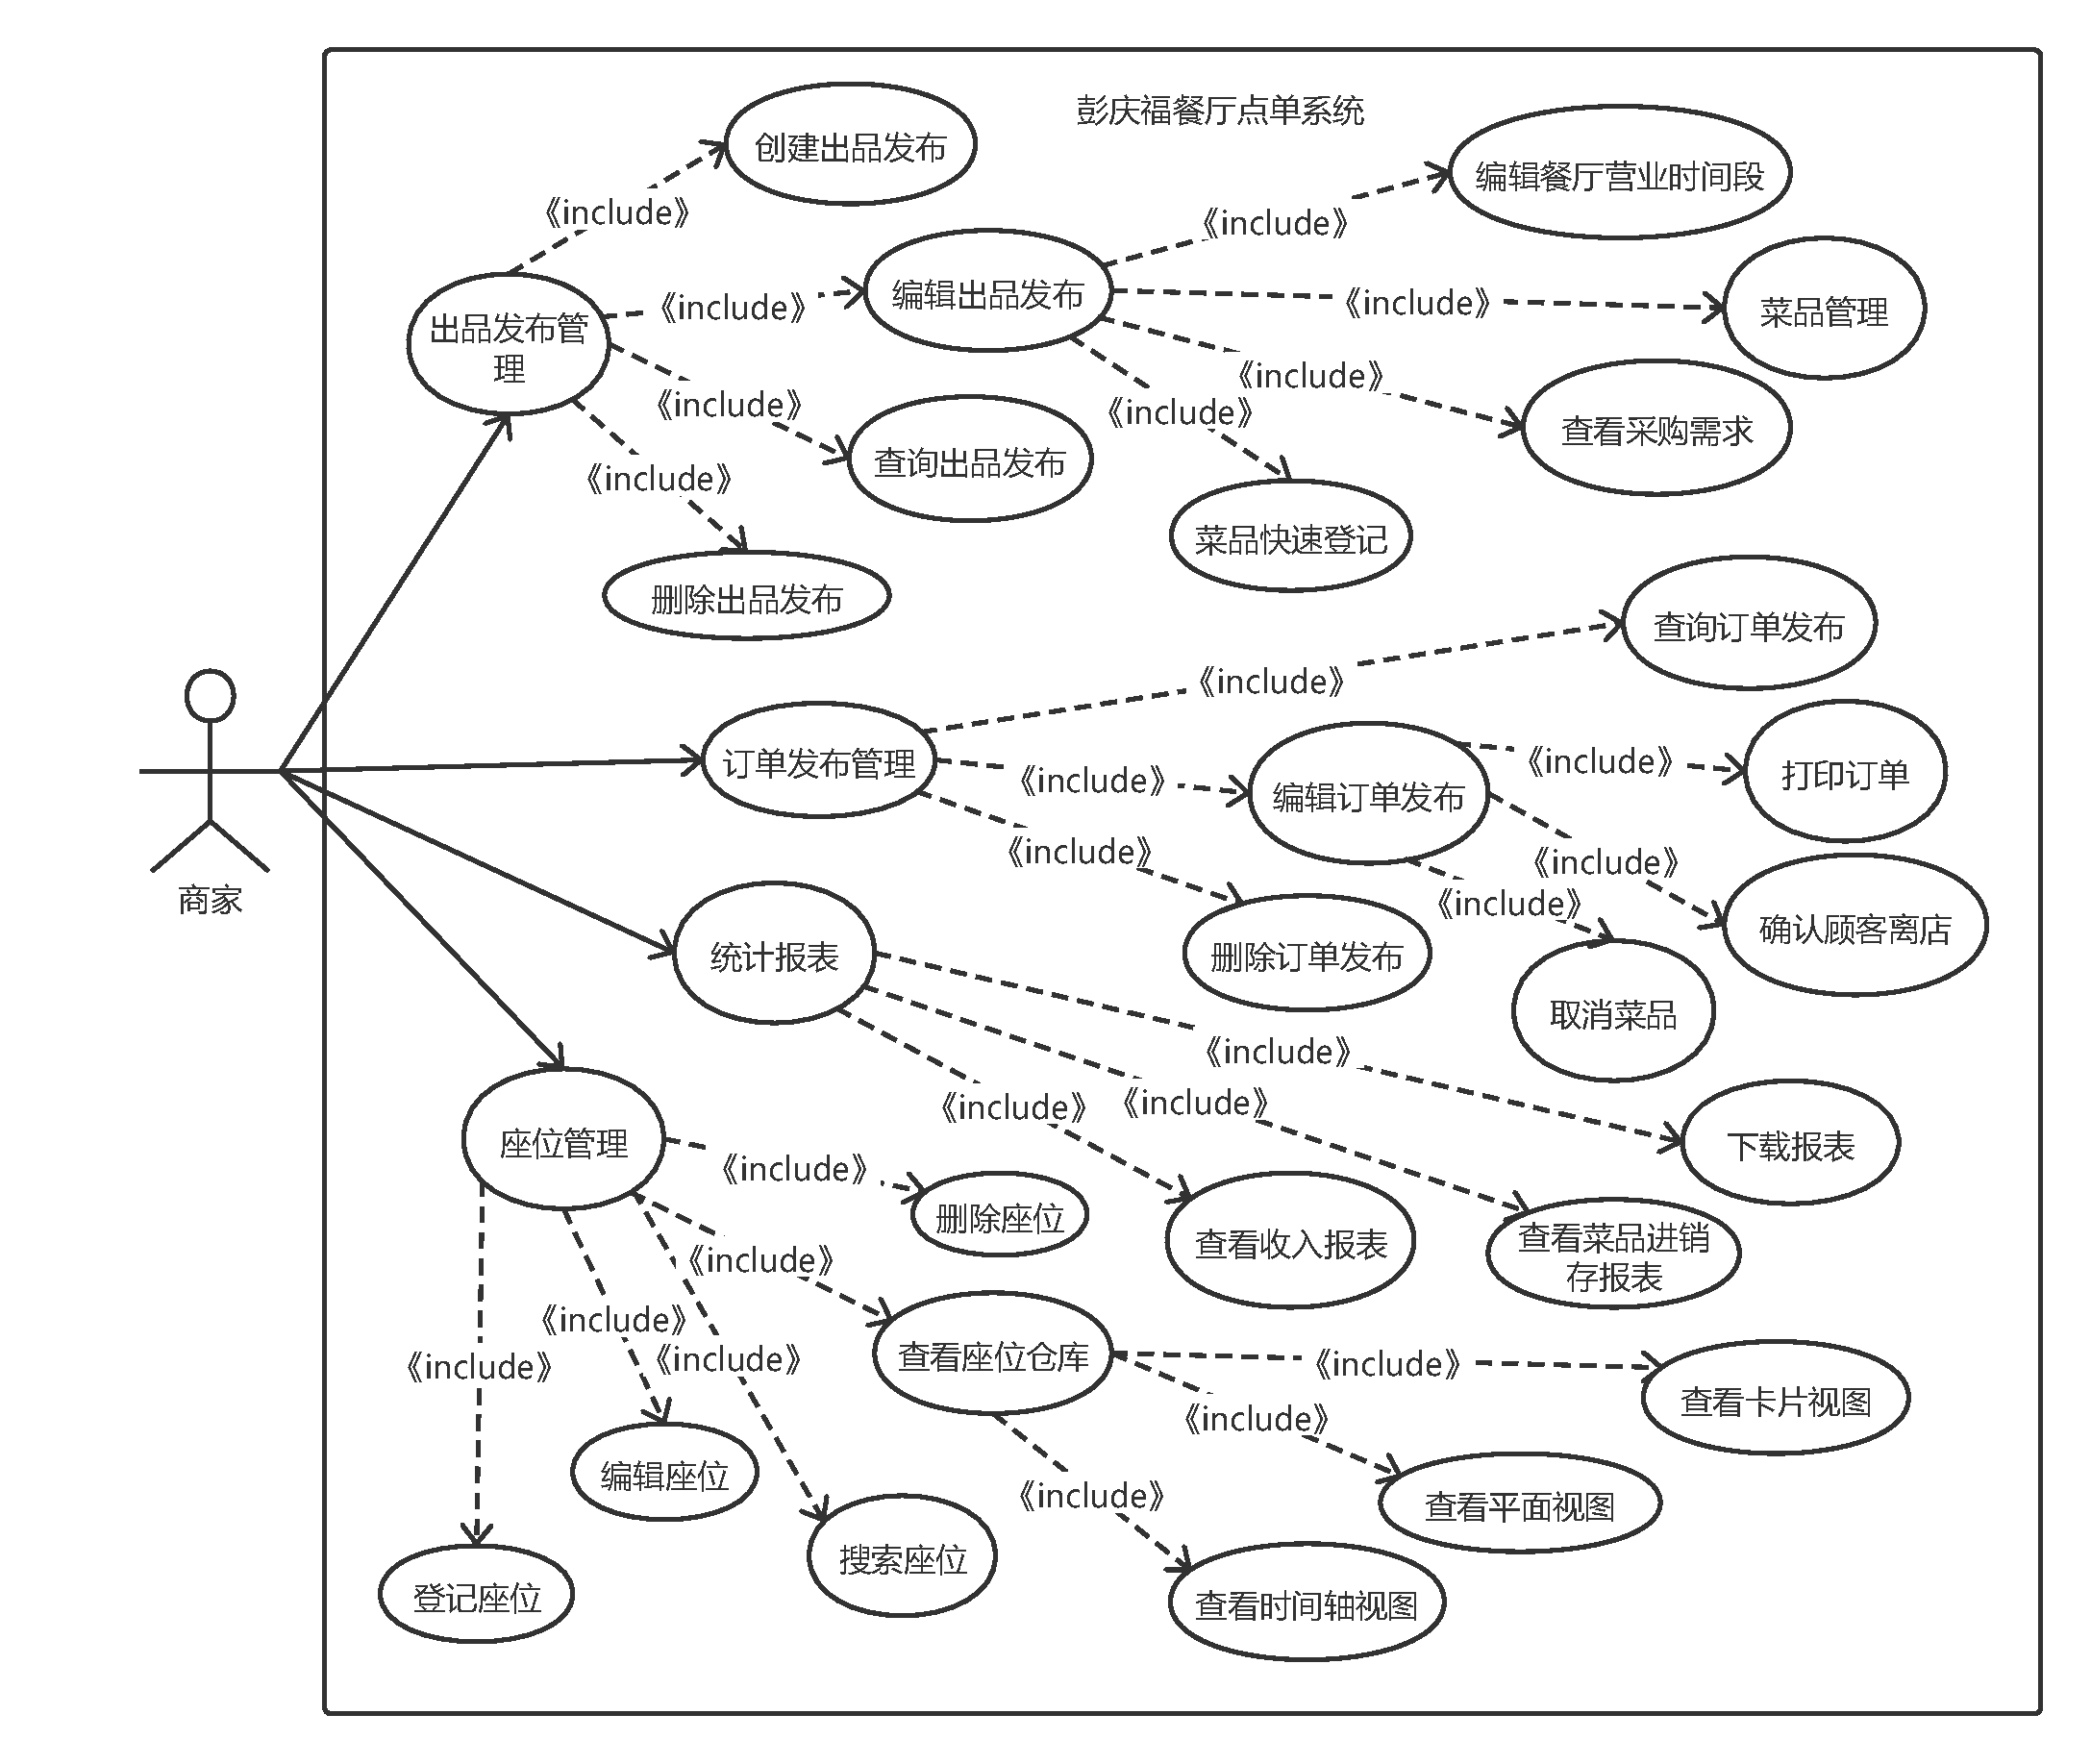
\includegraphics[width=5in]{FIGs/chapter3/seller.pdf}
  \caption{商家管理模块用例图}\label{fig_sellerCH3}
\end{figure}

商家功能需求部分,是彭庆福餐厅点单系统中主要由Web端网页操作的部分,其用例图如图~\ref{fig_sellerCH3}所示,主要包括了出品发布管理、订单发布管理、座位管理、统计报表等功能,商家成功登录系统后,可以根据需要进行不同的操作来管理、运营餐厅。

下面将详细描述关于商家管理平台的几个重要用例。

如表~\ref{table:uc5}所示,其描述了商家对出品发布管理的具体过程,出品发布由商家创建,它包含每日计划营业时间段、对菜品的分类管理、对库存的增补管理等。商家在成功登录系统后点击筛选发布中的出品发布,可以看到餐厅历史所有的出品发布列表,可以根据需要创建新的出品发布,设置餐厅每日的营业时间、菜单等。可以根据需要搜索筛选特定的出品发布,点击某一出品发布标题,可以查看该出品发布的详情并进行管理更新。

对于创建好的出品计划,商家可以进行查看,包括出品时间、当日的营业时间段、要出售的产品、计划份数、订单份数等;也可以进行相应管理,包括更新餐厅当日的营业时间段,可以添加、修改、删除多段时间,增删改当日要销售的菜品(包括单个菜品、套餐等);也可以查看采购需求,根据库存提示进行相应的库存补充。商家将需要修改的发布内容都修改完成后,点击“更新出品发布”按钮,发布才会更新,这样帮助商家减少误操作,避免引发不必要的错误,相当于二次确认。创建新的出品发布时,可以复用已有的出品发布内容,只需要修改出品日期,系统会自动记录复用的出品发布内容并进行复用,商家可以在原有的内容基础上进行更新。

\begin{table}[htbp!]
  \footnotesize
  \centering
  \caption{出品发布管理用例表}
  \vspace{2mm}
  \begin{tabular}{cp{11.5cm}}
   \hline
   \ ID & UC6 \\ 
   \hline
   \ 名称 & 出品发布管理 \\ 
   \hline
   \ 参与者 & 商家,目标是查看并管理所有出品发布。 \\ 
   \hline
   \ 优先级 & 高 \\ 
   \hline
   \ 触发条件 & 用户需要查看餐厅的所有出品发布。 \\ 
   \hline
   \ 前置条件 & 用户成功登录彭庆福餐厅点单系统,并拥有管理出品发布的权限。 \\ 
   \hline
   \ 后置条件 & 出品发布列表内容更新。 \\ 
   \hline
   \multirow{2}{*}{正常流程}
    & 1.	已成功登录的用户进入发布页面,点击出品发布。\\
    & 2.	系统显示餐厅所有的出品发布列表。\\
    & 3.	用户输入出品发布关键字,选择搜索。\\
    & 4.	系统显示与之相关的出品发布。\\
    & 5.  用户点击某一出品发布。\\
    & 6.  系统显示该出品发布详情。\\
    & 7.  用户查看详情,并选择相应操作。\\
    & 8.  系统保存用户修改并更新界面。\\
    & 用户可以重复步骤3-8,直至完成所有要搜索、查询和修改的出品发布。\\
   \hline
   \multirow{2}{*}{扩展流程}
    & 3a. 用户选择添加出品发布,并输入内容:\\
    & ~~1.	若填写内容有误,系统提示正确格式。\\
    & ~~2.	填写无误,用户点击确定后,系统保存更改并更新出品发布列表。\\
    & 4a. 要查询的出品发布不存在:\\
    & ~~1.	系统提示该出品发布不存在。\\
    & 7a. 用户选择编辑出品发布,并填写修改内容:\\
    & ~~1.	用户修改餐厅当日营业时间段,系统保存更改并更新界面。\\
    & ~~2.	用户对当日菜品做修改,增删菜品,系统保存更改并更新界面。\\
    & ~~3.	用户查看采购需求,并对当日库存不足的菜品进行快速登记,系统保存更改并更新界面。\\
    & 7b. 用户选择删除该出品发布:\\
    & ~~1.	系统请用户再次确认,确认成功后系统删除该出品发布并更新界面内容。\\
    & ~~2.	再次确认时用户选择取消,系统不做更改,返回详情界面。\\
  \hline
  \ 特殊需求 & 无 \\ 
  \hline
  \end{tabular}
  \label{table:uc5}
\end{table}

如下表~\ref{table:uc6}所示,其描述了商家对订单发布进行管理的具体过程,订单发布由系统自动创建。有顾客下单时,订单发布就会新增一条订单与之对应,它包含订单号、座位、就餐人数、顾客用餐时间、到店时间以及订单的菜品详情、总金额等。商家在成功登录系统后,点击筛选发布中的订单发布就可以看到餐厅历史所有的订单发布列表,点击具体订单发布查看订单发布详情并进行管理。

商家进入某个订单详情页面后,可以看到订单类型、状态、订单号、座位、顾客用餐时间等顾客信息和所点菜品信息,根据订单状态以及个人权限进行相应操作,比如修改订单的就餐人数。对于已经支付的订单,商家可以点击确认离店结束订单状态,可以查看订单的相应评论、个人评论,回复顾客评论。

\begin{table}[htbp!]
  \footnotesize
  \centering
  \caption{订单发布管理用例表}
  \vspace{2mm}
  \begin{tabular}{cp{11.5cm}}
   \hline
   \ ID & UC7 \\ 
   \hline
   \ 名称 & 订单发布管理 \\ 
   \hline
   \ 参与者 & 商家,目标是查看并管理所有订单发布。 \\ 
   \hline
   \ 优先级 & 高 \\ 
   \hline
   \ 触发条件 & 用户需要查看餐厅的所有订单发布。 \\ 
   \hline
   \ 前置条件 & 用户成功登录彭庆福餐厅点单系统,并拥有管理订单发布的权限。 \\ 
   \hline
   \ 后置条件 & 订单发布列表内容更新。 \\ 
   \hline
   \multirow{2}{*}{正常流程}
    & 1.	已成功登录的用户进入发布页面,点击订单发布。\\
    & 2.	系统显示餐厅所有的订单发布列表。\\
    & 3.	用户输入订单发布关键字,选择搜索。\\
    & 4.	系统显示与之相关的订单发布。\\
    & 5.  用户点击某一订单发布。\\
    & 6.  系统显示该订单发布详情。\\
    & 7.  用户查看详情,并选择相应操作。\\
    & 8.  系统保存用户修改并更新界面。\\
    & 用户可以重复步骤3-8,直至完成所有要搜索、查询和修改的订单发布。\\
   \hline
   \multirow{2}{*}{扩展流程}
    & 4a. 要查询的订单发布不存在:\\
    & ~~1.	系统提示该订单发布不存在。\\
    & 7a. 用户选择编辑订单发布,并填写修改内容:\\
    & ~~1.	用户打印订单详情,系统打印出包含菜品信息及金额的账单。\\
    & ~~2.	用户取消订单内某菜品,系统保存更改并更新界面。\\
    & ~~3.	当顾客用餐完成且订单状态为已支付时,用户点击确认离店,系统保存更改并更新界面。\\
    & 7b. 用户选择删除该订单发布:\\
    & ~~1.	系统请用户再次确认,确认成功后系统删除该订单发布并更新界面内容。\\
    & ~~2.	再次确实时用户选择取消,系统不做更改,返回详情界面。\\
  \hline
  \ 特殊需求 & 无 \\ 
  \hline
  \end{tabular}
  \label{table:uc6}
\end{table}

如下表~\ref{table:uc7}所示,其描述了商家对座位管理的具体过程,商家在成功登录系统后,点击座位库可以查看所有座位,选择不同视图进行座位列表查看,点击具体座位可以查看详情并进行管理。

\begin{table}[htbp!]
  \footnotesize
  \centering
  \caption{座位管理用例表}
  \vspace{2mm}
  \begin{tabular}{cp{11.5cm}}
   \hline
   \ ID & UC8 \\ 
   \hline
   \ 名称 & 座位管理 \\ 
   \hline
   \ 参与者 & 商家,目标是查看并管理所有座位。 \\ 
   \hline
   \ 优先级 & 高 \\ 
   \hline
   \ 触发条件 & 用户需要查看餐厅的所有座位。 \\ 
   \hline
   \ 前置条件 & 用户成功登录彭庆福餐厅点单系统,并拥有管理座位的权限。 \\ 
   \hline
   \ 后置条件 & 座位库内容更新。 \\ 
   \hline
   \multirow{2}{*}{正常流程}
    & 1.	已成功登录的用户进入座位库。\\
    & 2.	系统显示座位库内的所有座位。\\
    & 3.	用户选择不同的视图查看。\\
    & 4.	系统根据选择显示不同视图的座位列表。\\
    & 5.  用户输入关键字,选择搜索。\\
    & 6.  系统显示所有相关的座位。\\
    & 7.  用户点击登记座位,填写座位编号、座位数、座位类型,并确认。\\
    & 8.  系统保存内容,并更新座位库。\\
    & 9.	用户点击某座位删除。\\
    & 10.	系统保存内容,并更新座位库。\\
    & 11.  用户点击某一座位。\\
    & 12.  系统显示该座位详情,包括座号、二维码、状态、座位数、类型以及占用情况记录。\\
    & 13.  用户查看详情,并选择相应操作。\\
    & 14.  系统保存用户修改并更新界面。\\
    & 用户可以重复步骤3-14,直至完成所有要操作的规则。\\
   \hline
   \multirow{2}{*}{扩展流程}
    & 3a. 用户选择时间轴视图:\\
    & ~~1.	系统显示当天各个座位被占用的时刻图,用户可以筛选时间查看不同日期座位的时间轴视图。\\
    & ~~2.	用户点击某个座位的某状态下的时间块。\\
    & ~~3.	系统跳转到相关的订单发布详情页面。\\
    & 3b. 用户选择平面视图:\\
    & ~~1.	系统显示各个座位在地图上的坐标信息,用户可以编辑平面视图,管理地图上各个座位的相关信息。\\
    & 3c. 用户选择卡片视图:\\
    & ~~1.	系统显示当天各个座位基本信息,用户可以查看座位信息、设置座位状态。\\
    & 5a. 搜索座位不存在:\\
    & ~~1.	系统提示该座位不存在。\\
    & 7a. 若填写内容有误:\\
    & ~~1.	系统显示错误,并提示正确格式。\\
    & 13a. 用户选择下载二维码:\\
    & ~~1.	系统下载该座位的二维码到本地。\\
    & 13b. 用户筛选不同日期:\\
    & ~~1.	系统根据日期显示该座位的占用情况记录。\\
  \hline
  \ 特殊需求 & 无 \\ 
  \hline
  \end{tabular}
  \label{table:uc7}
\end{table}

商家可以从三种不同的视图来查看和管理座位库。

默认视图为卡片视图,可以看到座位列表以卡片形式呈现,商家可以根据座号、座位状态、时间来组合筛选座位,可以修改座位状态,进行座位的增删改,也可以点击座位详情进行查看具体信息。商家可以选择时间轴视图,查看不同日期的餐厅座位被预订、占用以及空闲状态,可以在相应的状态上点击进入到相关的订单发布中查看具体的订单详情。商家也可以选择平面视图,编辑座位或者餐厅的实际地址信息,在高德地图或者自己上传的餐厅平面图上进行打点、画圈,将地理位置与座位卡片相关联。

\begin{table}[htbp!]
  \footnotesize
  \centering
  \caption{统计报表用例表}
  \vspace{2mm}
  \begin{tabular}{cp{11.5cm}}
   \hline
   \ ID & UC9 \\ 
   \hline
   \ 名称 & 统计报表 \\ 
   \hline
   \ 参与者 & 商家,目标是统计报表。 \\ 
   \hline
   \ 优先级 & 高 \\ 
   \hline
   \ 触发条件 & 用户需要查看餐厅收入、菜品进销存的报表。 \\ 
   \hline
   \ 前置条件 & 用户成功登录彭庆福餐厅点单系统,并拥有统计报表的权限。 \\ 
   \hline
   \ 后置条件 & 统计报表内容更新。 \\ 
   \hline
   \multirow{2}{*}{正常流程}
    & 1.	已成功登录的用户进入统计报表页面。\\
    & 2.	系统显示当日收入报表。\\
    & 3.	用户点击菜品进销存报表。\\
    & 4.	系统显示当日进销存报表。\\
    & 5.  用户点击下载报表。\\
    & 6.  系统下载当前报表。\\
    & 用户可以重复步骤3-6,直至完成所有要操作的规则。\\
   \hline
   \multirow{2}{*}{扩展流程}
    & 3a. 用户选择不同时间筛选:\\
    & ~~1.	系统根据时间显示不同的报表。\\
  \hline
  \ 特殊需求 & 无 \\ 
  \hline
  \end{tabular}
  \label{table:uc8}
\end{table}

如表~\ref{table:uc8}所示,其描述了商家统计报表的具体过程,商家在成功登录系统后,点击统计报表查看收入报表和菜品进销存报表,点击下载可以保存报表。\\

\subsection{系统非功能性需求分析}
\begin{table}[htbp!]
  \footnotesize
  \centering
  \caption{非功能性需求表}
  \vspace{2mm}
  % l - left, r - right, c - center. | means one vertical line
  \begin{tabular}{cp{9.5cm}}
  % \midrule
  \hline
  \multirow{3}{3.5cm}{
    \textbf{可用性}
    }&1. 为符合用户的正常操作习惯,将不同类型操作分开,不同用户群体的使用端分开。\\
    &2. 系统需要在用户完成某些操作后给出对应消息提醒,比如提示弹窗、二次确认弹框等。\\
    &3. 系统在必要情况下需提供使用帮助文档或者说明页面,使用户在使用系统时可以降低操作难度。\\
  \hline
  \multirow{2}{3.5cm}{
    \textbf{系统性能}
    }&1. 系统在同一时间内响应需要超过190个请求。\\
    &2. 系统能在用户操作时间的0.4秒内提供其相应反馈。\\
  \hline
  \multirow{2}{3.5cm}{
    \textbf{支持性}
    }&系统能在Windows、Mac OS、Linux等主流操作系统上运行,并且能在手机端正常使用,在微信客户端、支付宝客户端以及主流浏览器(比如IE、Chrome、Opera、Safari等)上良好运行。\\
  \hline
  \multirow{2}{3.5cm}{
    \textbf{可靠性}
    }&服务器有可能会宕机,需要在多台服务器中部署服务,使得某台服务器宕机后,服务依然可以正常使用。\\
  \hline
  \multirow{2}{3.5cm}{
    \textbf{安全性}
    }&1. 系统需要确保用户个人资料的安全性,其中包含用户密码、电话、个人基本情况等。\\
    &2. 系统通过权限管理来控制用户权限,使得不同类型用户的操作权限可以不同。\\
  \hline
  \end{tabular}
  \label{table:systemsRequirement}
\end{table}
如表~\ref{table:systemsRequirement}所示,是系统对非功能性需求的要求,包括可用性、系统性能、支持性、可靠性以及安全性。

\section{顾客功能执行流程设计}
设计该系统是为了能够高效、便捷解决顾客在日常生活中因为用餐产生的各种问题,也是为了商家能够节省时间,准确定位到每一个订单,更好地统计菜品种类库存、顾客历史订单等数据~\cite{battistini1999order}。

\begin{figure}[htbp!]
  \centering
  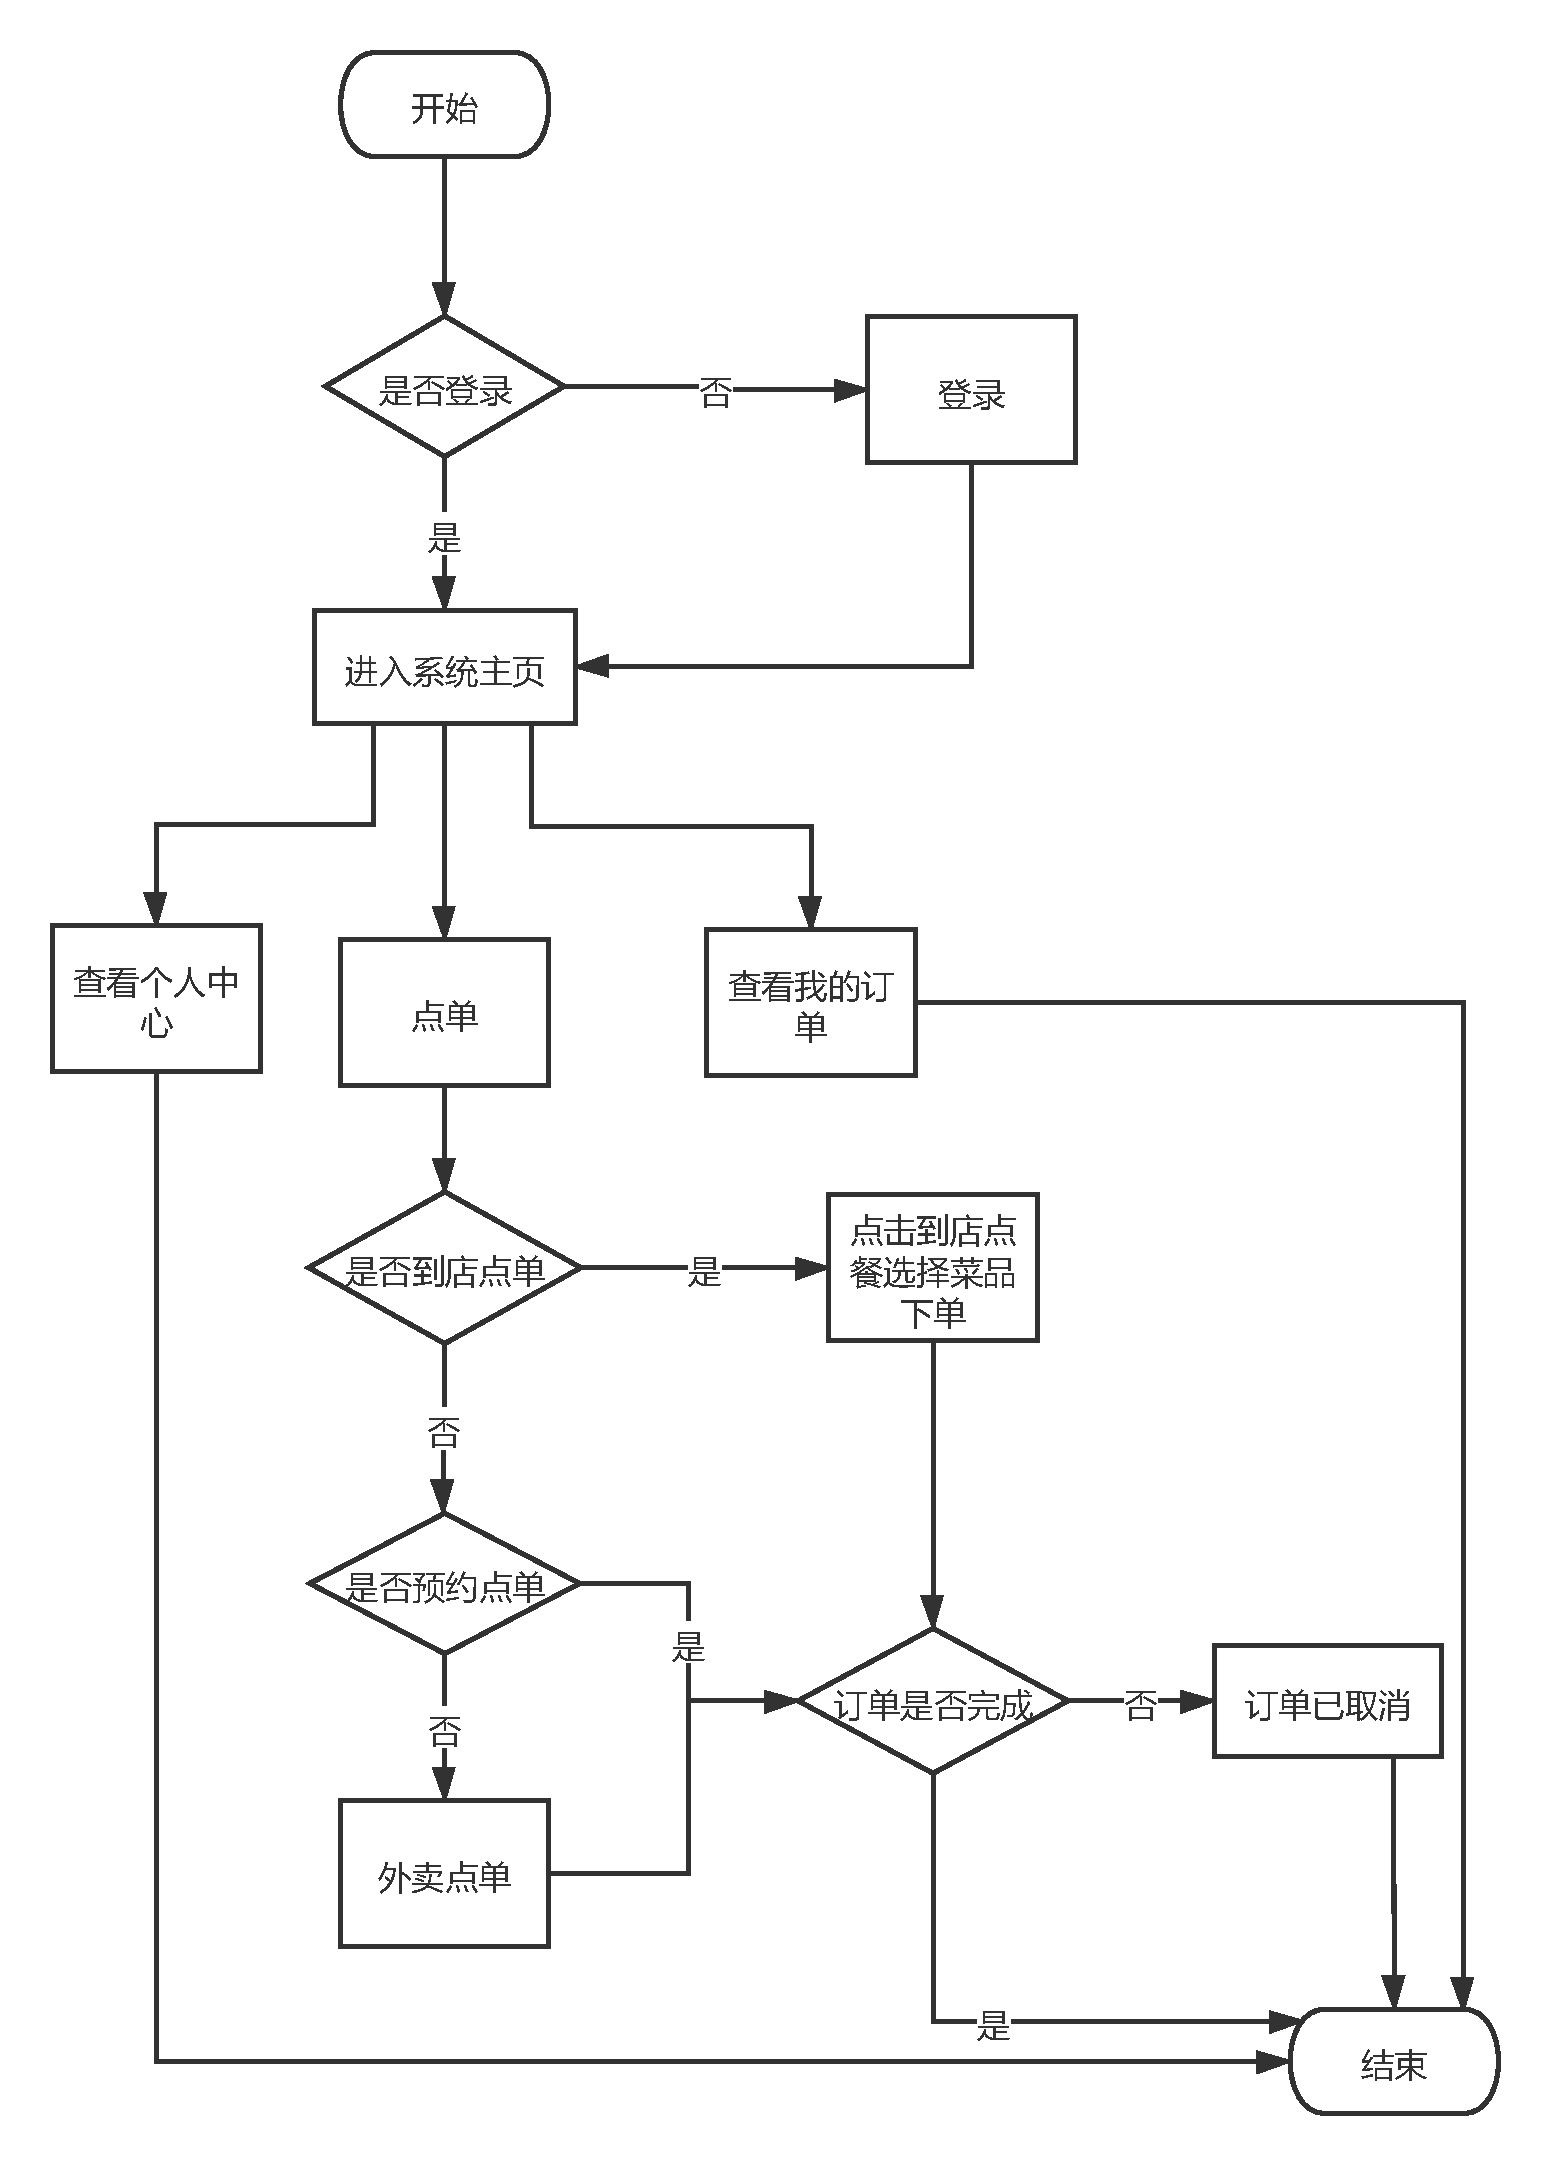
\includegraphics[width=4in]{FIGs/chapter3/flow.pdf}
  \caption{顾客主页功能的执行流程图}\label{fig_flowCH3}
\end{figure}

如图~\ref{fig_flowCH3}所示,这是顾客访问系统的主要执行流程图,以下对该图进行详细描述:
\begin{enumerate}
  \item 顾客首先进入系统主页,如果没有登录则跳转到登录页面。
  \item 系统提供点单、查看个人中心、查看我的订单功能,顾客可以选择查看信息,若只是查看信息则查看完成后结束整个流程,若要点单则转向步骤3。
  \item 顾客是否在餐厅运营期间且到店进行点餐,若是则可扫描座位上二维码下单,如果不是则可以预约点单或者外卖点单。
  \item 如果订单完成或者取消则结束整个流程。
\end{enumerate}

\section{系统概要设计}
本节主要介绍了彭庆福餐厅点单系统的总体设计、系统部署、数据库设计等信息。\\
\subsection{总体设计}
该系统中,顾客可以通过关注商家的微信公众号,使用公众号内自定义的菜单栏进入系统,也可以使用支付宝、浏览器扫一扫座位号进入点单页面~\cite{swain2019electrical}。顾客点单页面使用HTML5页面展示,商家在PC端设置店铺状态、菜品管理以及订单管理,系统部署在服务器集群上,有五台服务器分工服务,实现负载均衡。为了使用户在高并发环境下也可以正常进行点单、下单等操作,保证良好的用户体验,系统使用了分布式缓存Redis存储用户一般经常访问的数据内容,以减轻查询数据库的压力~\cite{balalaie2016microservices}。商家会实时获取到用户下单的各个类型订单,以便及时准备菜品并送达,系统采用云平台在消息队列中存储订单,监听云打印机的在线情况方便实时打印用户订单。

系统的支付功能采用新型支付方式——移动支付,其中包括微信、支付宝支付,用户在通过微信、支付宝或者浏览器界面进行到店、预定、外卖订餐后,可以选择在线支付或者等待食物送达再付款~\cite{liu2015application}。系统采用的微信支付使用H5支付、Native支付和JASPI支付,系统通过移动端网页展示菜品,用户在当前网页中确认使用微信支付时,商家会发起本次服务转至微信相关平台进行支付。

如图~\ref{fig_logicCH3}所示,系统的逻辑视图可以分为H5对象、Controller对象和Web对象,对象之间双向通信。H5对象的责任是进行顾客点单,例如它使用了菜单显示给用户菜品详情,使用用户管理进行个人中心的管理,使用订单进行订单的生成、查看;Controller对象负责进行一些逻辑功能的处理,并调用Service层的服务接口,进而与数据库进行交互;Web对象的责任是进行商家管理,例如它使用了菜单管理对菜单和餐厅营业时间进行管理,使用用户管理进行餐厅位置、电话、简介等的管理,使用订单进行订单查看、管理,使用统计报表对每日收支以及菜品进销存表进行查看。

\begin{figure}[htbp!]
  \centering
  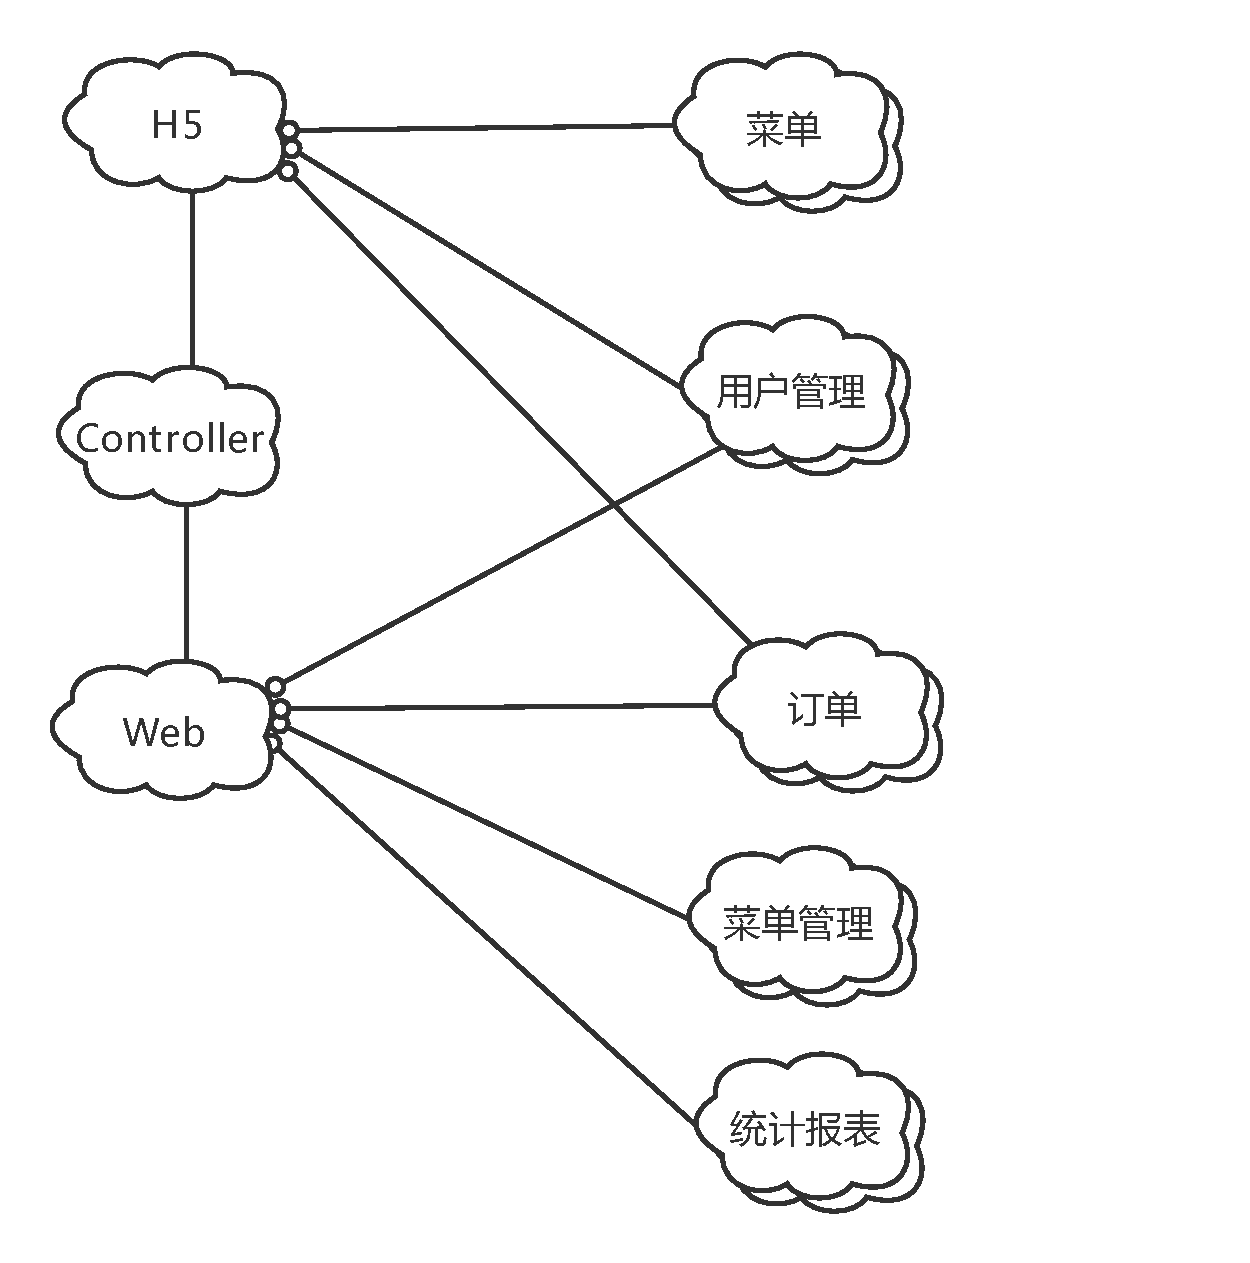
\includegraphics[width=3in]{FIGs/chapter3/logic.pdf}
  \caption{彭庆福点单系统逻辑视图}\label{fig_logicCH3}
\end{figure}

\begin{figure}[htbp!]
  \centering
  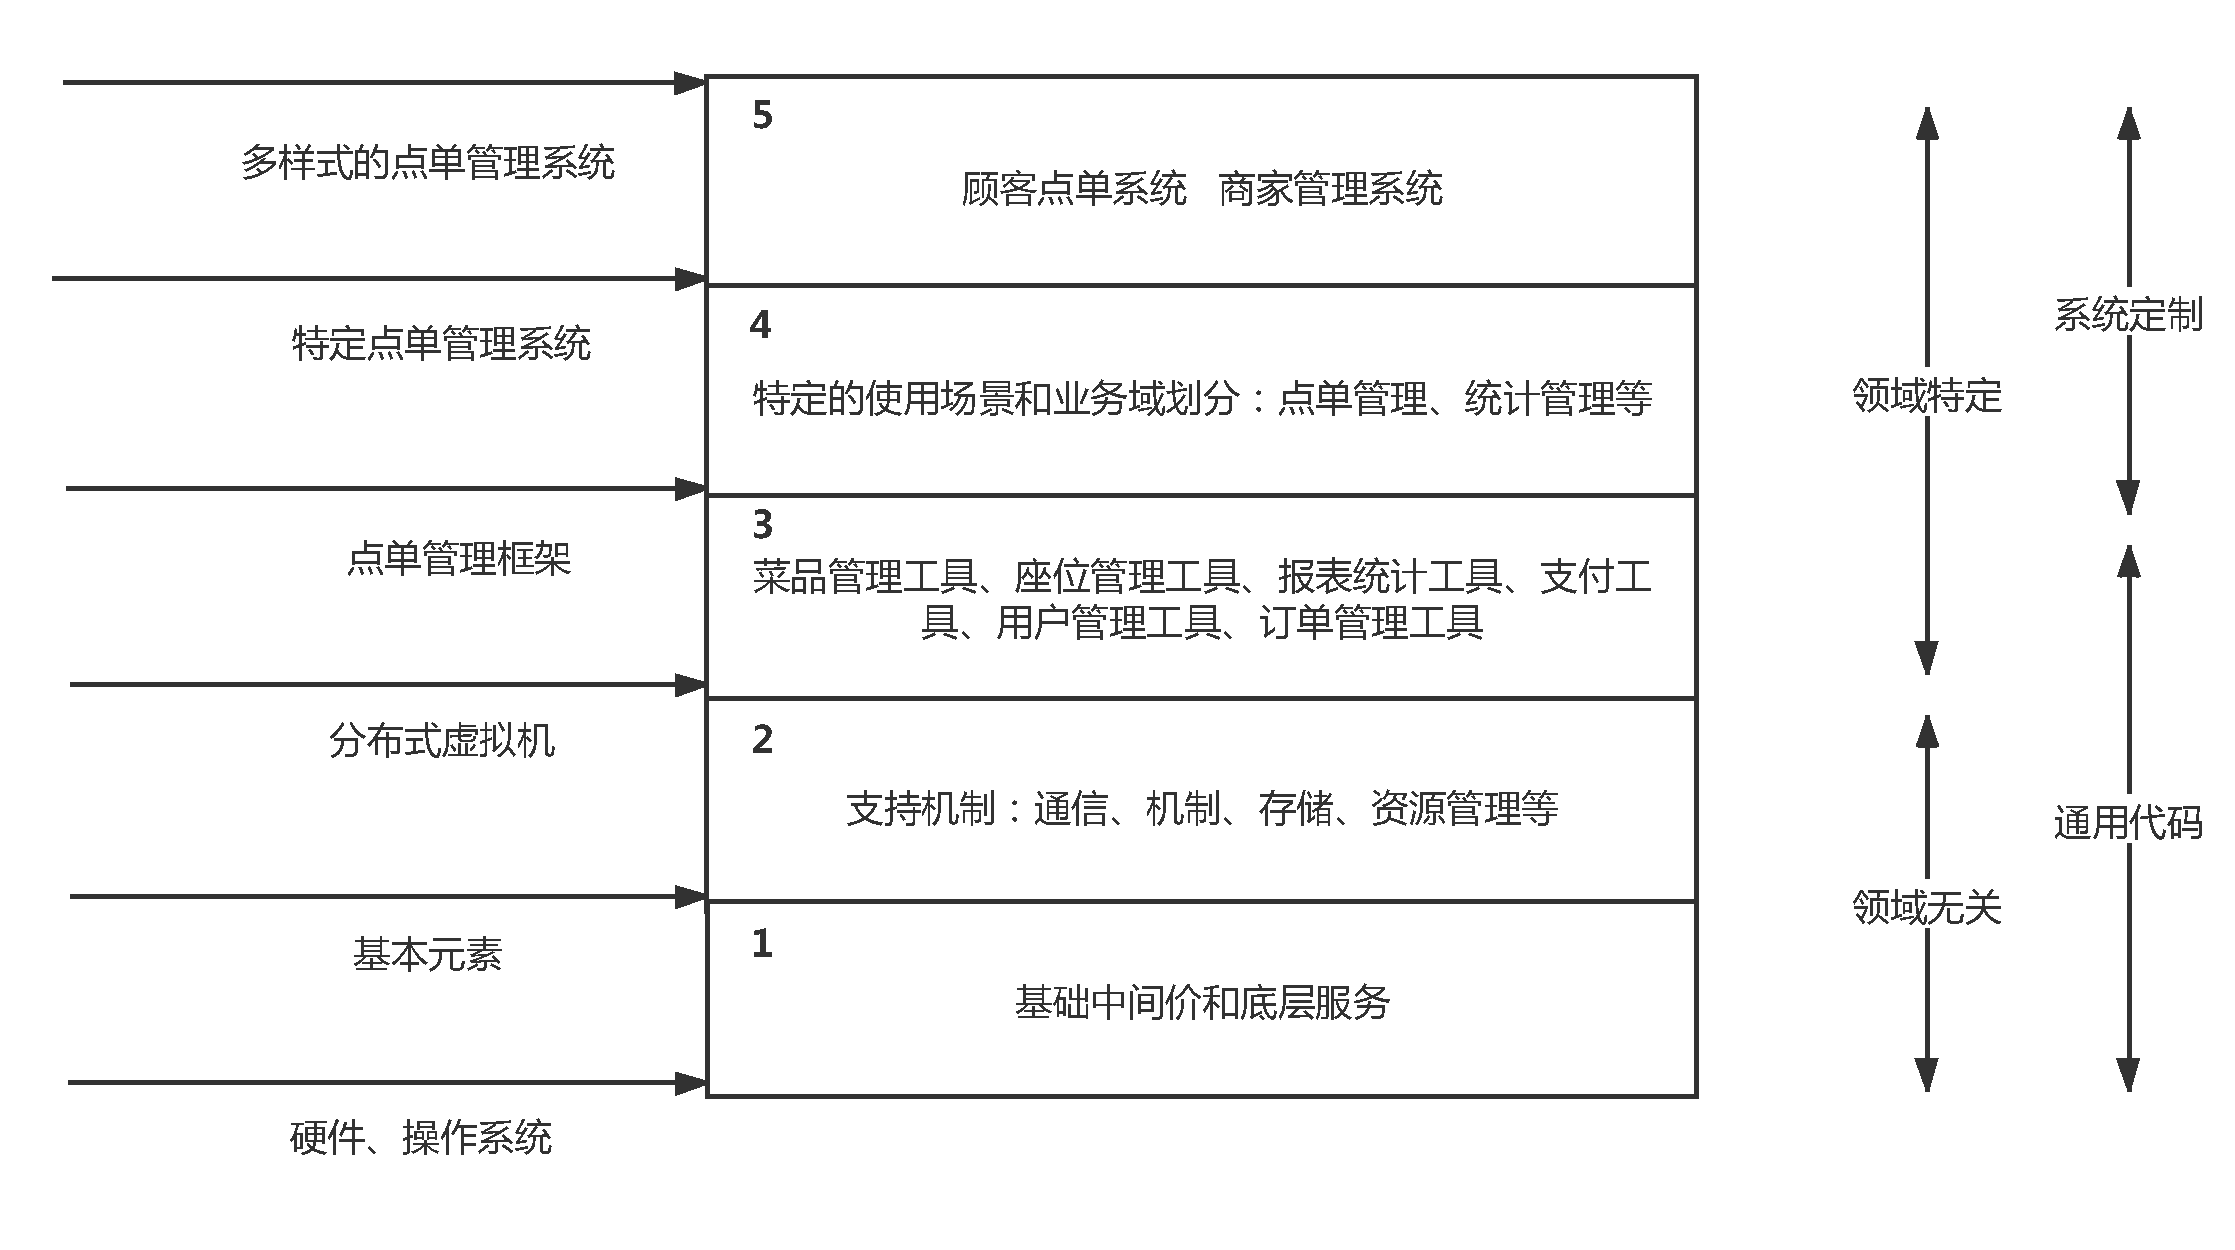
\includegraphics[width=5in]{FIGs/chapter3/develop.pdf}
  \caption{彭庆福点单系统开发视图}\label{fig_developCH3}
\end{figure}

彭庆福点单系统产品线的5个分层开发的组织结构如图~\ref{fig_developCH3}所示,系统的一二层组成了独立的、覆盖整个产品线的基础设施;第三层为基础设施增加了点单管理框架,组成了特定领域的软件架构形式;在此基础上,第四层构建了特定场景域选择,基本涵盖了系统所需功能;第五层依赖于用户和产品内容,包含了功能齐全的用户接口、外部系统接口等。

\begin{figure}[htb]
  \centering
  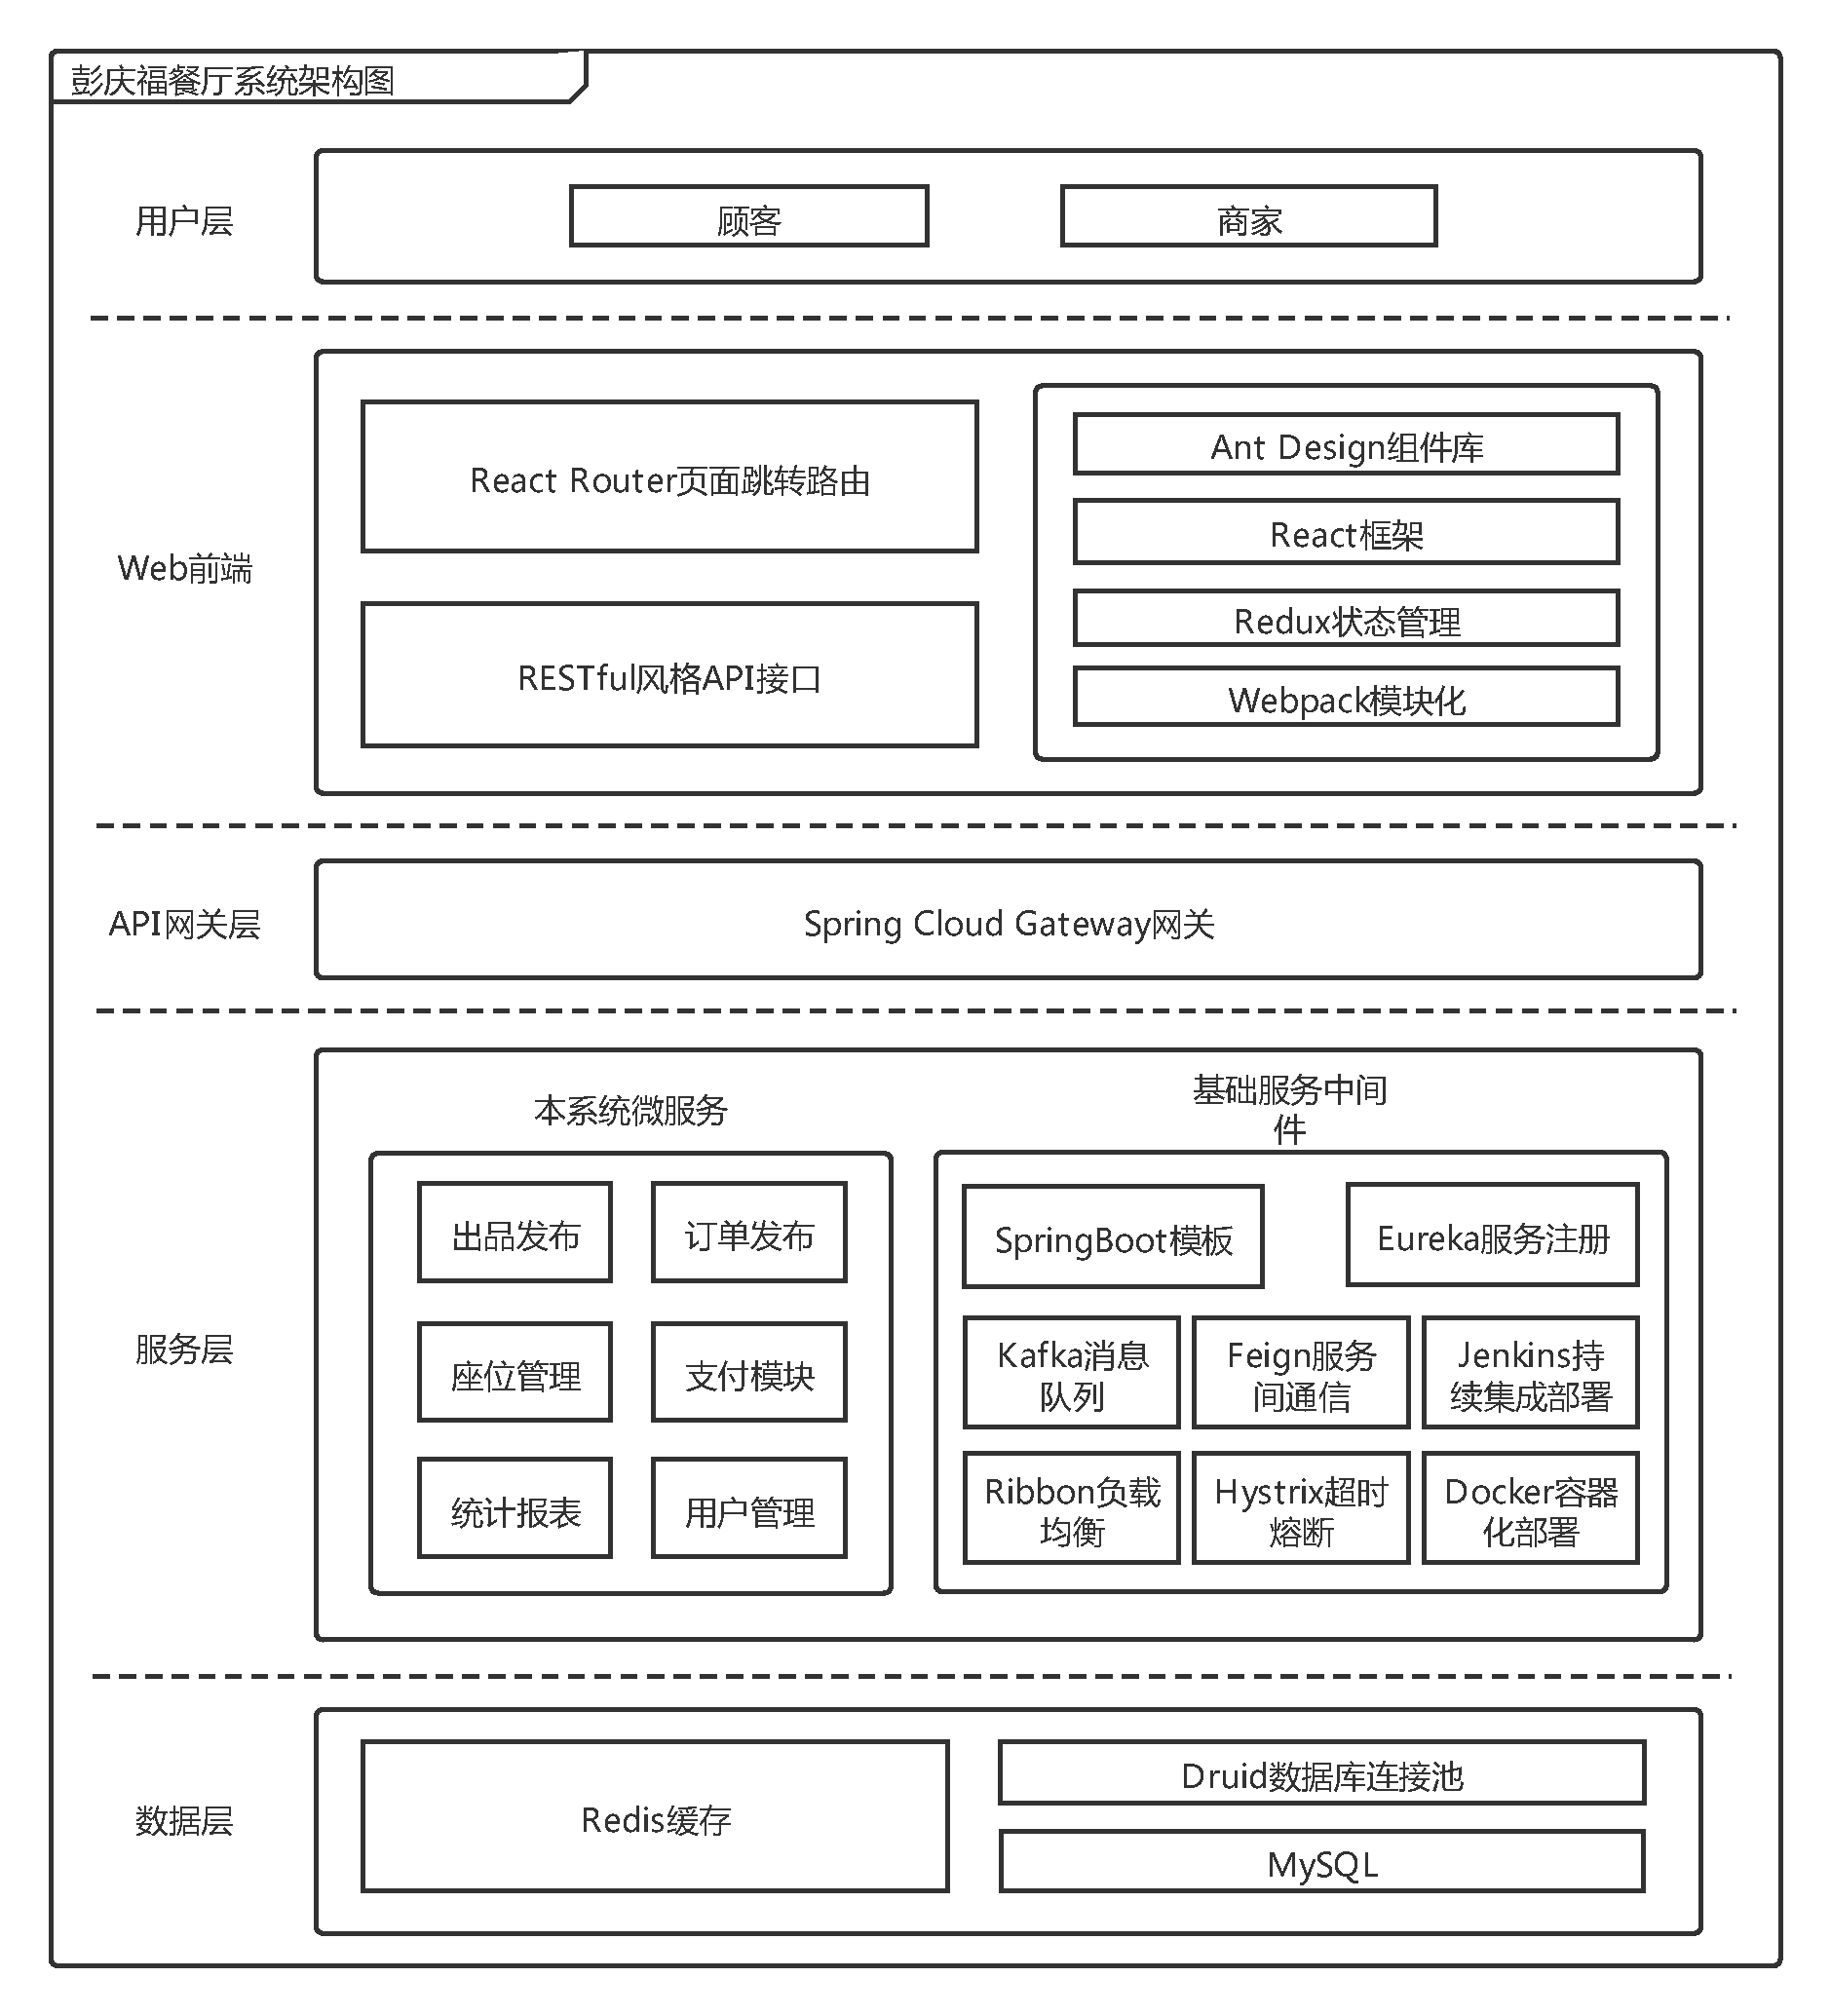
\includegraphics[width=5in]{FIGs/chapter3/all.pdf}
  \caption{系统架构图}\label{fig_allCH3}
\end{figure}

如图~\ref{fig_allCH3}所示的彭庆福餐厅点单系统架构图,系统一共可以分为用户层、Web前端、API网关层、服务层和数据层。在用户层中,考虑到顾客和商家的不同使用习惯,点单部分和管理部分分别设计成了手机浏览(H5界面)和PC端网页浏览的形式。Web前端项目由React框架搭建,可以快速渲染、局部刷新,搭配Redux技术进行第三方通信,通过把数据存储在Store里,达到状态、数据流的统一管理。页面跳转路由使用了React Router实现,并使用RESTful风格的API接口,使用了Ant Design组件库antd使得UI界面统一、美观,使用Webpack作为前端打包工具,把资源统一打包成少量文件,并结合插件进行语法转换。

API网关层负责接收Web前端发来的接口请求,使用了Spring Cloud Gateway网关,向下调用服务层提供的请求来响应,并将处理后的请求结果返还给前端~\cite{venugopal2017containerized}。服务层是由一些基础服务中间件和本系统功能拆分的微服务所组成,包括出品发布服务、订单发布服务、座位管理服务、支付模块服务、统计报表服务和用户管理服务,每个服务都具有相应的功能来对应特定接口,服务之间还存在着不同的依赖,除此之外还有一些第三方服务。

数据层主要负责数据持久化,存储着彭庆福餐厅点单系统的各类数据信息,包括顾客、订单详情、菜品、订单、计划、座位、商家等信息。\\

\subsection{部署架构}
\begin{figure}[htbp!]
  \centering
  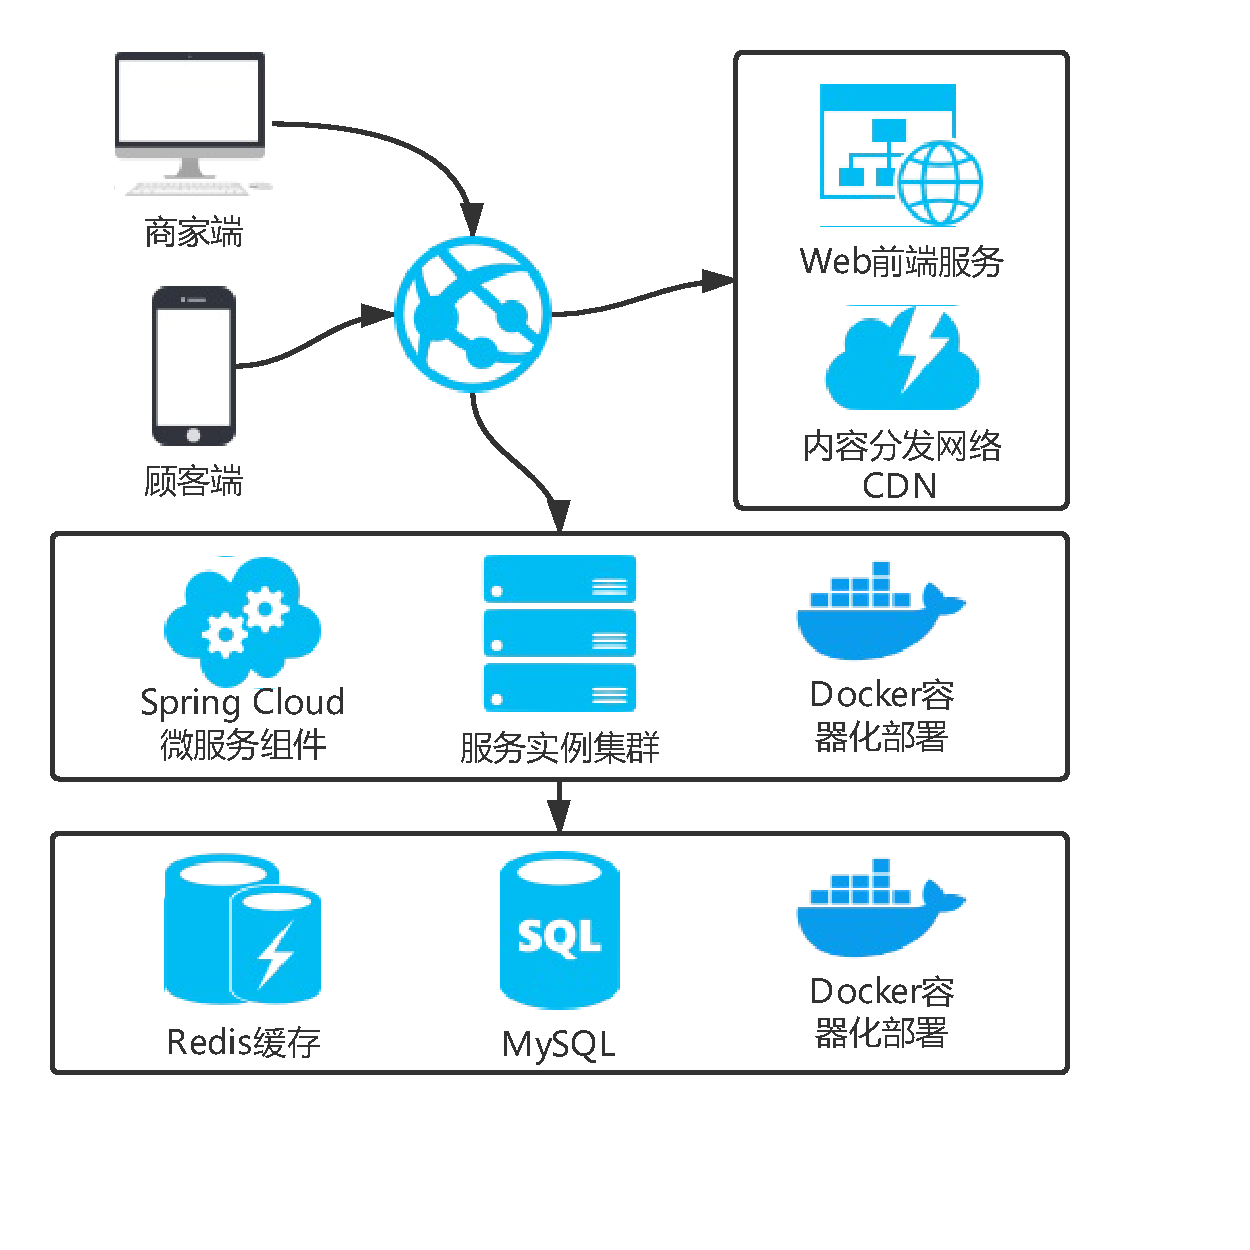
\includegraphics[width=4.5in]{FIGs/chapter3/physics.pdf}
  \caption{彭庆福餐厅点单系统物理视图}\label{fig_physicsCH3}
\end{figure}

彭庆福餐厅点单系统的部署结构主要分为三个部分:Web前端服务层、后端微服务层、数据库层,如图~\ref{fig_physicsCH3}所示。

商家端或顾客端设备获取Web前端资源,请求会发送到Web前端服务层,这一层处理所有前端的脚本与静态资源。本层部署时首先从持续集成系统CI获取构建完整的部署包,用该部署包分组刷新服务实例,其他静态资源上传到内容分发网络CDN。

同样商家端或顾客端设备访问后端数据,请求会发到后端微服务层,这一层处理所有RESTful动态数据请求。本层部署时同样会先从持续集成系统CI获取构建完整的部署包后分组刷新服务实例,在刷新时需要先更新Spring Cloud微服务组件再更新具体业务逻辑服务。在部署组件服务和业务逻辑服务时,统一使用Docker进行容器化部署。

后端微服务层在处理请求时,访问数据库的请求会发到数据库层,这一层主要做持久化数据的存储和访问,使用缓存提高访问效率。本层部署对象包括MySQL关系型数据库和基于Redis的缓存服务,部署时二者都使用Docker的官方镜像。此外,Redis部署时需要对缓存做预热操作。

\section{数据库设计}
\begin{figure}[htbp!]
  \centering
  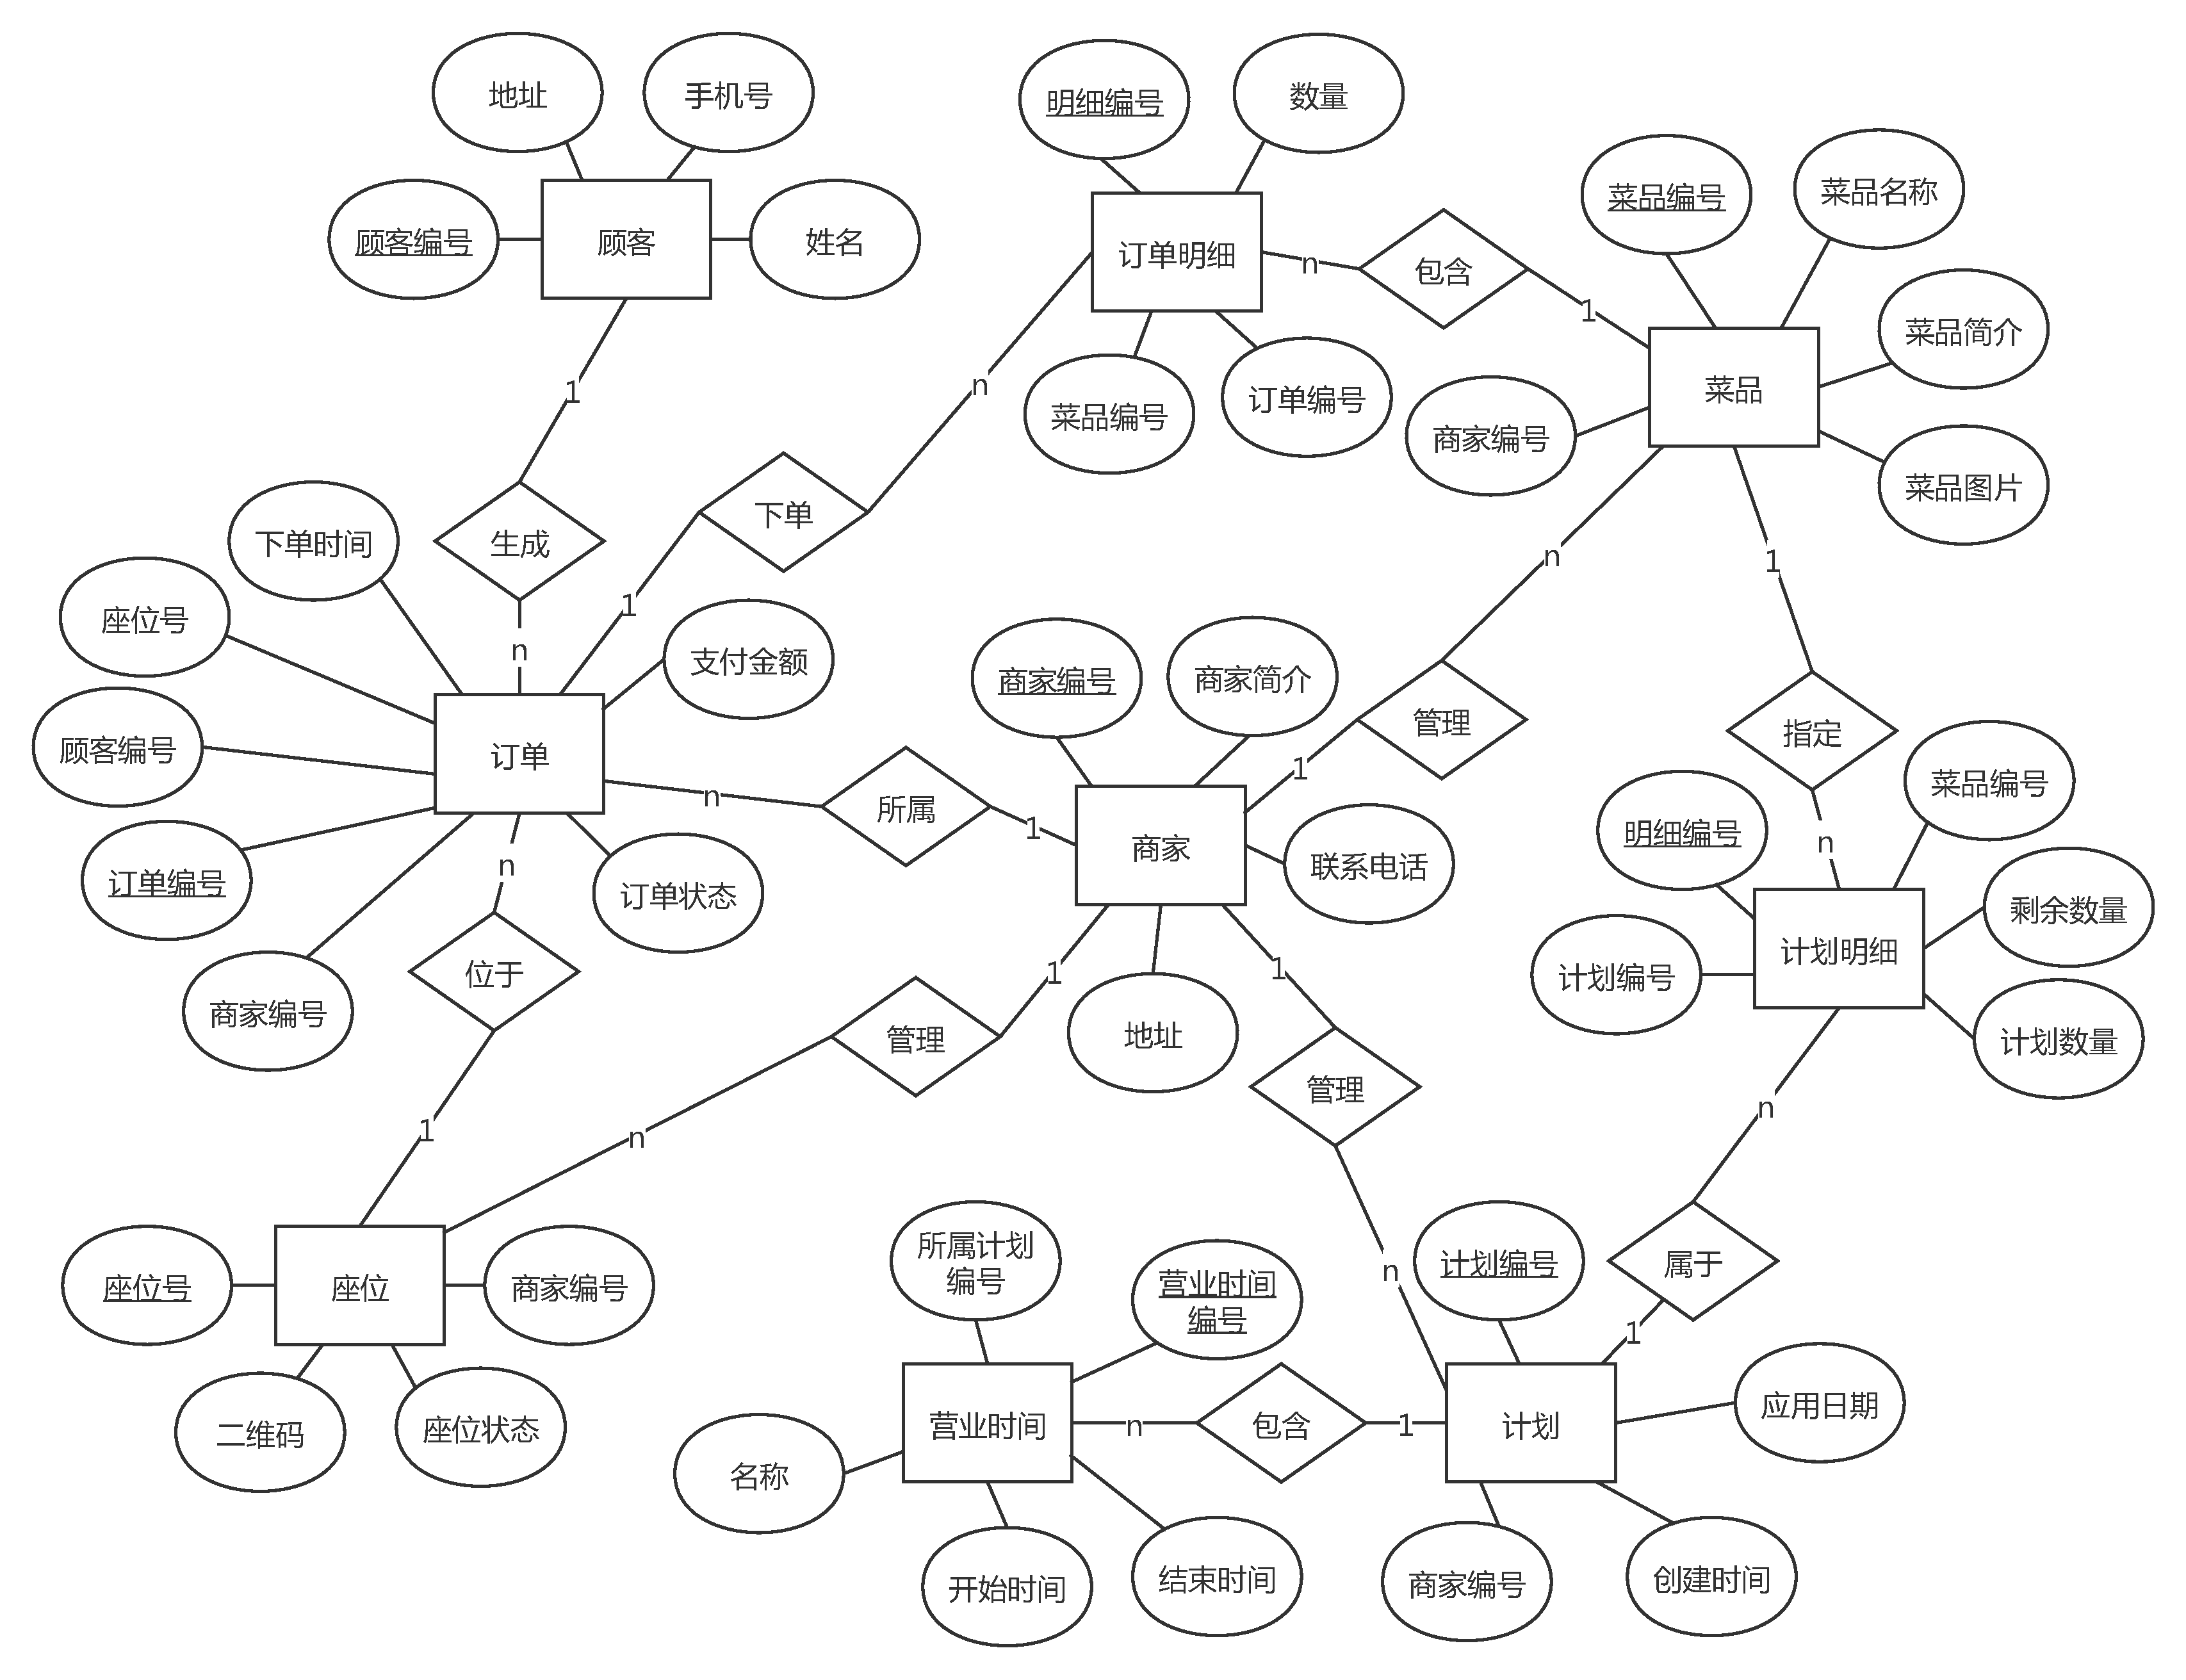
\includegraphics[width=5in]{FIGs/chapter3/ER.pdf}
  \caption{彭庆福餐厅实体关系图}\label{fig_ERCH3}
\end{figure}

结合系统的模块设计与业务需求,本项目将数据库表大致分成了四个部分,分别是订单、菜品、计划以及用户信息。

彭庆福餐厅点单系统的数据库实体关系图如图~\ref{fig_ERCH3}所示,包括顾客、商家、订单、订单明细、座位、菜品、计划、计划明细、营业时间等几个实体,实体之间存在一对多的关系。

\begin{table}[htbp!]\footnotesize
  \centering
  \caption{顾客实体数据库表Customer}
  \vspace{2mm}
  \begin{tabular}{lllll}
  \toprule
  \textbf{名称}&\textbf{类型}&\textbf{长度}&\textbf{允许空值}&\textbf{描述}\\
  \midrule 
  customerId& bigint& 30& No& 顾客编号\\
  \hline
  name& varchar& 30& No& 顾客姓名\\
  \hline
  phone& varchar& 20& Yes& 联系手机号码\\
  \hline
  address& varchar& 50& Yes& 配送地址\\
  \bottomrule
  \end{tabular}
  \label{table:ER1}
\end{table}

顾客实体是对所有就餐客人的抽象,主要保存用户编号、姓名、手机号、配送地址等属性。
表~\ref{table:ER1}是描述顾客实体的数据库表Customer,主键为顾客编号customerId,主要记录顾客的个人信息,方便顾客下单。为提高查询效率,在主键上建立索引。

\begin{table}[htbp!]\footnotesize
  \centering
  \caption{商家实体数据库表Merchant}
  \vspace{2mm}
  \begin{tabular}{lllll}
  \toprule
  \textbf{名称}&\textbf{类型}&\textbf{长度}&\textbf{允许空值}&\textbf{描述}\\
  \midrule 
  merchantId& bigint& 30& No& 商家编号\\
  \hline
  introduction& varchar& 200& No& 商家简介\\
  \hline
  phone& varchar& 20& No& 联系电话\\
  \hline
  address& varchar& 50& Yes& 店面地址\\
  \bottomrule
  \end{tabular}
  \label{table:ER2}
\end{table}

商家实体用于描述餐厅的线下实体店,主要保存商家编号、商家简介、地址和联系电话等属性。
表~\ref{table:ER2}是描述商家实体的数据库表Merchant,主键为商家编号merchantId。为提高查询效率,在主键上建立索引。

\begin{table}[htbp!]\footnotesize
  \centering
  \caption{座位实体数据库表Seat}
  \vspace{2mm}
  \begin{tabular}{lllll}
  \toprule
  \textbf{名称}&\textbf{类型}&\textbf{长度}&\textbf{允许空值}&\textbf{描述}\\
  \midrule 
  seatId& bigint& 30& No& 座位号\\
  \hline
  merchantId& bigint& 30& No& 所属商家编号\\
  \hline
  qrcode& varchar& 20000& No& 二维码\\
  \hline
  state& int& 5& No& 座位状态\\
  \bottomrule
  \end{tabular}
  \label{table:ER3}
\end{table}

座位实体是对可用座位的抽象,主要保存座位号、二维码、座位状态和所属商家编号等属性。
表~\ref{table:ER3}是描述座位实体的数据库表Seat,主键为座位号seatId。为提高查询效率,在主键和所属商家编号上分别建立索引。

\begin{table}[htbp!]\footnotesize
  \centering
  \caption{菜品实体数据库表Product}
  \vspace{2mm}
  \begin{tabular}{lllll}
  \toprule
  \textbf{名称}&\textbf{类型}&\textbf{长度}&\textbf{允许空值}&\textbf{描述}\\
  \midrule 
  productId& bigint& 30& No& 菜品编号\\
  \hline
  merchantId& bigint& 30& No& 所属商家编号\\
  \hline
  name& varchar& 20& No& 菜品名称\\
  \hline
  introduction& varchar& 200& Yes& 菜品简介\\
  \hline
  image& varchar& 20000& Yes& 菜品图片\\
  \bottomrule
  \end{tabular}
  \label{table:ER4}
\end{table}

菜品实体是对菜单上可选菜品的抽象,主要保存菜品编号、菜品简介、菜品图片和所属商家编号等属性。
表~\ref{table:ER4}是描述菜品实体的数据库表Product,主键为菜品编号productId。为提高查询效率,在主键和所属商家编号上分别建立索引。

\begin{table}[htbp!]\footnotesize
  \centering
  \caption{订单实体数据库表Order}
  \vspace{2mm}
  \begin{tabular}{lllll}
  \toprule
  \textbf{名称}&\textbf{类型}&\textbf{长度}&\textbf{允许空值}&\textbf{描述}\\
  \midrule 
  orderId& bigint& 30& No& 订单编号\\
  \hline
  seatId& bigint& 30& No& 就餐座位号\\
  \hline
  merchantId& bigint& 30& No& 所属商家编号\\
  \hline
  customerId& bigint& 30& No& 下单顾客编号\\
  \hline
  createdAt& timestamp& 100& No& 创建时间\\
  \hline
  state& int& 5& No& 订单状态\\
  \hline
  price& float& 10& No& 支付金额\\
  \bottomrule
  \end{tabular}
  \label{table:ER5}
\end{table}

订单实体是对客户顾客就餐产生订单的抽象,主要保存订单编号、订单状态、下单时间、支付金额、所属商家编号、来源顾客编号、就餐座位号等属性。
表~\ref{table:ER5}是描述订单实体的数据库表Order,主键为orderId。为提高查询效率,在主键、所属商家编号和下单客户编号上分别建立索引。

\begin{table}[htbp!]\footnotesize
  \centering
  \caption{订单明细实体数据库表OrderItem}
  \vspace{2mm}
  \begin{tabular}{lllll}
  \toprule
  \textbf{名称}&\textbf{类型}&\textbf{长度}&\textbf{允许空值}&\textbf{描述}\\
  \midrule 
  orderItemId& bigint& 30& No& 订单明细编号\\
  \hline
  orderId& bigint& 30& No& 所属订单编号\\
  \hline
  productId& bigint& 30& No& 下单菜品编号\\
  \hline
  quantity& int& 10& No& 下单数量\\
  \bottomrule
  \end{tabular}
  \label{table:ER6}
\end{table}

订单明细实体是对订单中选择的菜品进行抽象,主要保存所属订单编号、选择的菜品编号和数量等属性。
表~\ref{table:ER6}是描述订单明细实体的数据库表OrderItem,主键为orderItemId。为提高查询效率,在主键和所属订单编号上分别建立索引。

\begin{table}[htbp!]\footnotesize
  \centering
  \caption{计划实体数据库表Plan}
  \vspace{2mm}
  \begin{tabular}{lllll}
  \toprule
  \textbf{名称}&\textbf{类型}&\textbf{长度}&\textbf{允许空值}&\textbf{描述}\\
  \midrule 
  planId& bigint& 30& No& 编号\\
  \hline
  merchantId& bigint& 30& No& 所属商家编号\\
  \hline
  createTime& timestamp& 100& No& 创建时间\\
  \hline
  applyDate& date& 50& No& 应用日期\\
  \bottomrule
  \end{tabular}
  \label{table:ER7}
\end{table}

计划实体用于描述商家对菜品销售和营业时间的计划,主要保存计划编号、所属商家编号、创建时间和应用日期。
表~\ref{table:ER7}是描述计划实体的数据库表Plan,主键为计划编号planId,是出品计划的实体内容,需要与计划明细实体、营业时间实体相关联,从而为每个出品计划绑定菜单、库存数、计划数以及餐厅当日营业时间等内容。为提高查询效率,在主键和所属商家编号上分别建立索引。

\begin{table}[htbp!]\footnotesize
  \centering
  \caption{计划明细实体数据库表PlanItem}
  \vspace{2mm}
  \begin{tabular}{lllll}
  \toprule
  \textbf{名称}&\textbf{类型}&\textbf{长度}&\textbf{允许空值}&\textbf{描述}\\
  \midrule 
  planItemId& bigint& 30& No& 编号\\
  \hline
  planId& bigint& 30& No& 所属计划编号\\
  \hline
  productId& bigint& 30& No& 指定菜品编号\\
  \hline
  quantity& int& 10& No& 计划数量\\
  \hline
  remain& int& 10& No& 剩余数量\\
  \bottomrule
  \end{tabular}
  \label{table:ER8}
\end{table}

计划明细实体是指计划中包含的单个菜品销售计划,包括计划明细编号、所属计划编号、指定菜品编号、计划数量和剩余数量等属性。
表~\ref{table:ER8}是描述计划明细实体的数据库表PlanItem,主键为计划明细编号planItemId。为提高查询效率,在主键和所属计划编号上分别建立索引。

\begin{table}[htbp!]\footnotesize
  \centering
  \caption{营业时间实体数据库表PlanSlot}
  \vspace{2mm}
  \begin{tabular}{lllll}
  \toprule
  \textbf{名称}&\textbf{类型}&\textbf{长度}&\textbf{允许空值}&\textbf{描述}\\
  \midrule 
  planSlotId& bigint& 30& No& 编号\\
  \hline
  planId& bigint& 30& No& 所属计划编号\\
  \hline
  name& bigint& 30& No& 时间段名称\\
  \hline
  startTime& timestamp& 100& No& 开始时间\\
  \hline
  endTime& timestamp& 100& No& 结束时间\\
  \bottomrule
  \end{tabular}
  \label{table:ER9}
\end{table}

营业时间实体是对商家当日计划营业时间的抽象,主要保存营业时间编号、所属计划编号、时间段名称、开始时间和结束时间。
表~\ref{table:ER9}是描述营业时间实体的数据库表PlanSlot,主键为营业时间段编号planSlotId。为提高查询效率,在主键和所属计划编号上分别建立索引。

订单实体由顾客实体生成,被商家管理,一位顾客可以生成多个订单,商家也可以拥有多个订单,所以顾客与订单、商家与订单都是一对多的关系。
订单中可能包含不同数量的多种菜品,本系统使用订单明细实体来管理这种关系,订单与订单明细、菜品与订单明细都是一对多的关系。
商家可以管理菜品列表,也可以管理每日计划安排,所以商家与菜品、商家与计划实体都是一对多的关系。每个计划是指商家当日出品计划和营业时间段安排,包含不同数量的多个菜品,还包含多个不同营业时间段,因此计划实体与计划明细、计划实体与营业时间是一对多的关系~\cite{DBLP:conf/socpar/ShimmuraTA09}。

\section{本章小结}
本章对彭庆福餐厅点单系统的整体概要设计以及需求进行了分析。首先,对系统设计目标做了详细说明,分析其可行性,并通过系统整体结构图介绍了系统组成部分。接着,将项目需求从两个方面进行了阐述,包括功能需求——主要通过绘制用例图表对系统两类用户(顾客和商家)的需求进行了归纳,以及非功能需求——从可用性、系统性能、支持性、可靠性以及安全性进行了分析。并分析了较为重要的顾客功能执行的流程设计,从逻辑视图、开发视图、系统架构图等分析了系统模块交互,介绍了总体的架构设计和部署架构。通过实体关系图解释了系统的数据库设计,并对数据库表内容做了简要分析。

\chapter{彭庆福餐厅点单系统的详细设计与实现}
本章主要介绍了彭庆福餐厅点单系统的各个功能模块,分析了模块之间的依赖关系,具体描述了各模块的详细设计与实现细节。
\section{模块设计}
\begin{figure}[htbp!]
    \centering
    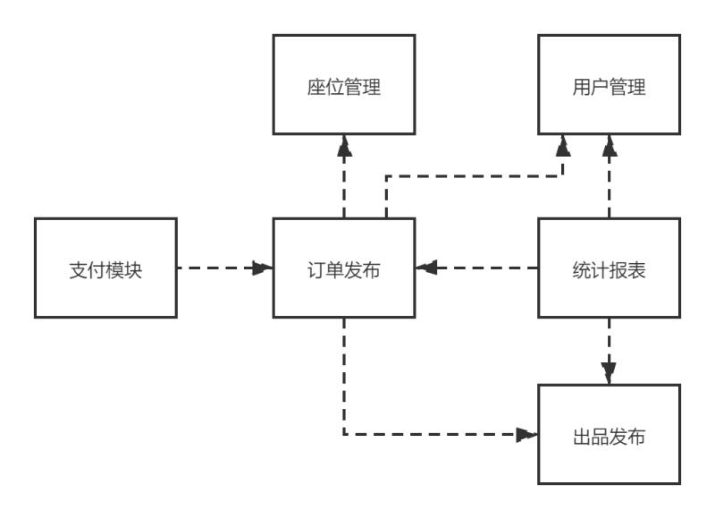
\includegraphics[width=4in]{FIGs/chapter4/model.pdf}
    \caption{系统模块结构图}\label{fig_model}
\end{figure}

彭庆福餐厅点单系统划分为六个模块,分别是订单发布模块、支付模块、用户管理模块、统计报表模块、座位管理模块和出品发布模块。模块之间的相互依赖如图~\ref{fig_model}所示,支付模块依赖订单发布模块,订单发布模块依赖座位管理模块、出品发布模块以及用户管理模块,统计报表模块依赖订单发布模块、出品发布模块以及用户管理模块。以下分别对不同模块进行介绍:

\begin{enumerate}
    \item 订单发布模块是整个系统中最主要的模块,它负责处理与顾客下单后的订单有关的操作,订单发布主要包括用户信息、座位信息以及菜品信息,对外提供订单列表、订单详情相关服务的接口。
    \item 支付模块依赖于订单发布,主要负责处理顾客支付时的支付安全和第三方支付,包括微信支付、支付宝支付等。
    \item 用户管理模块主要负责处理与用户各种信息有关的操作,系统一共有两大类用户,顾客和商家,用户管理模块主要对外提供顾客信息服务、角色服务、商家信息服务等接口。
    \item 统计报表模块主要负责收集、整合各个报表信息,主要对外提供不同时间段的收入报表、菜品进销存报表、下载报表的接口。
    \item 座位管理模块主要负责处理座位有关的操作,主要对外提供座位信息、座位二维码、座位状态等接口。
    \item 出品发布模块主要负责每日出品计划、菜品计划,用于每天的营业时间、菜品管理等问题的处理,主要对外提供商家营业信息、出品计划、菜品信息等接口。
\end{enumerate}

下面对这六个模块分别进行介绍。

\section{订单发布模块}
\subsection{订单发布模块介绍}
订单发布模块是整个系统中最主要的模块,它负责处理与顾客下单有关的操作,顾客可以选菜下单,创建订单、查询订单、取消订单,商家可以查看所有顾客订单以及对具体订单进行操作。订单发布主要包括用户信息、座位信息以及菜品信息,支付模块以及统计报表模块都需要依赖它。

订单发布模块需要多类状态综合判断,通过顾客状态(已到店、已离店)、商家处理订单状态、以及支付状态(待支付、已支付、支付失败)来决定订单状态(已提交待确认、进行中、已结束未评价、取消、已取消未评价、已结束已评价)。

订单发布模块会展示三种类型的订单详情,一种是到店订单类型,一种是预约订单类型,还有一种是外卖订单类型,多位顾客同时在线下单,后台会根据具体时间对订单排序生成特定订单编号。顾客每次下单都会根据不同类型生成相应订单,商家可以在订单发布里查看到所有的订单列表,点击具体订单可以查看订单详情,进行相应的操作,比如修改顾客用餐人数、确认顾客离店、打印菜单、结账等。\\

\subsection{订单发布模块详细设计}
订单发布模块包括顾客点单部分和商家管理订单部分,其中还涉及到了生产计划服务、用户服务、订单条目服务等。如图~\ref{fig_order}所示是订单发布模块的类图,主要实现了与订单相关的内容,需要依赖发布服务、生产计划服务、用户服务、订单条目等内容。

\begin{figure}[htbp!]
    \centering
    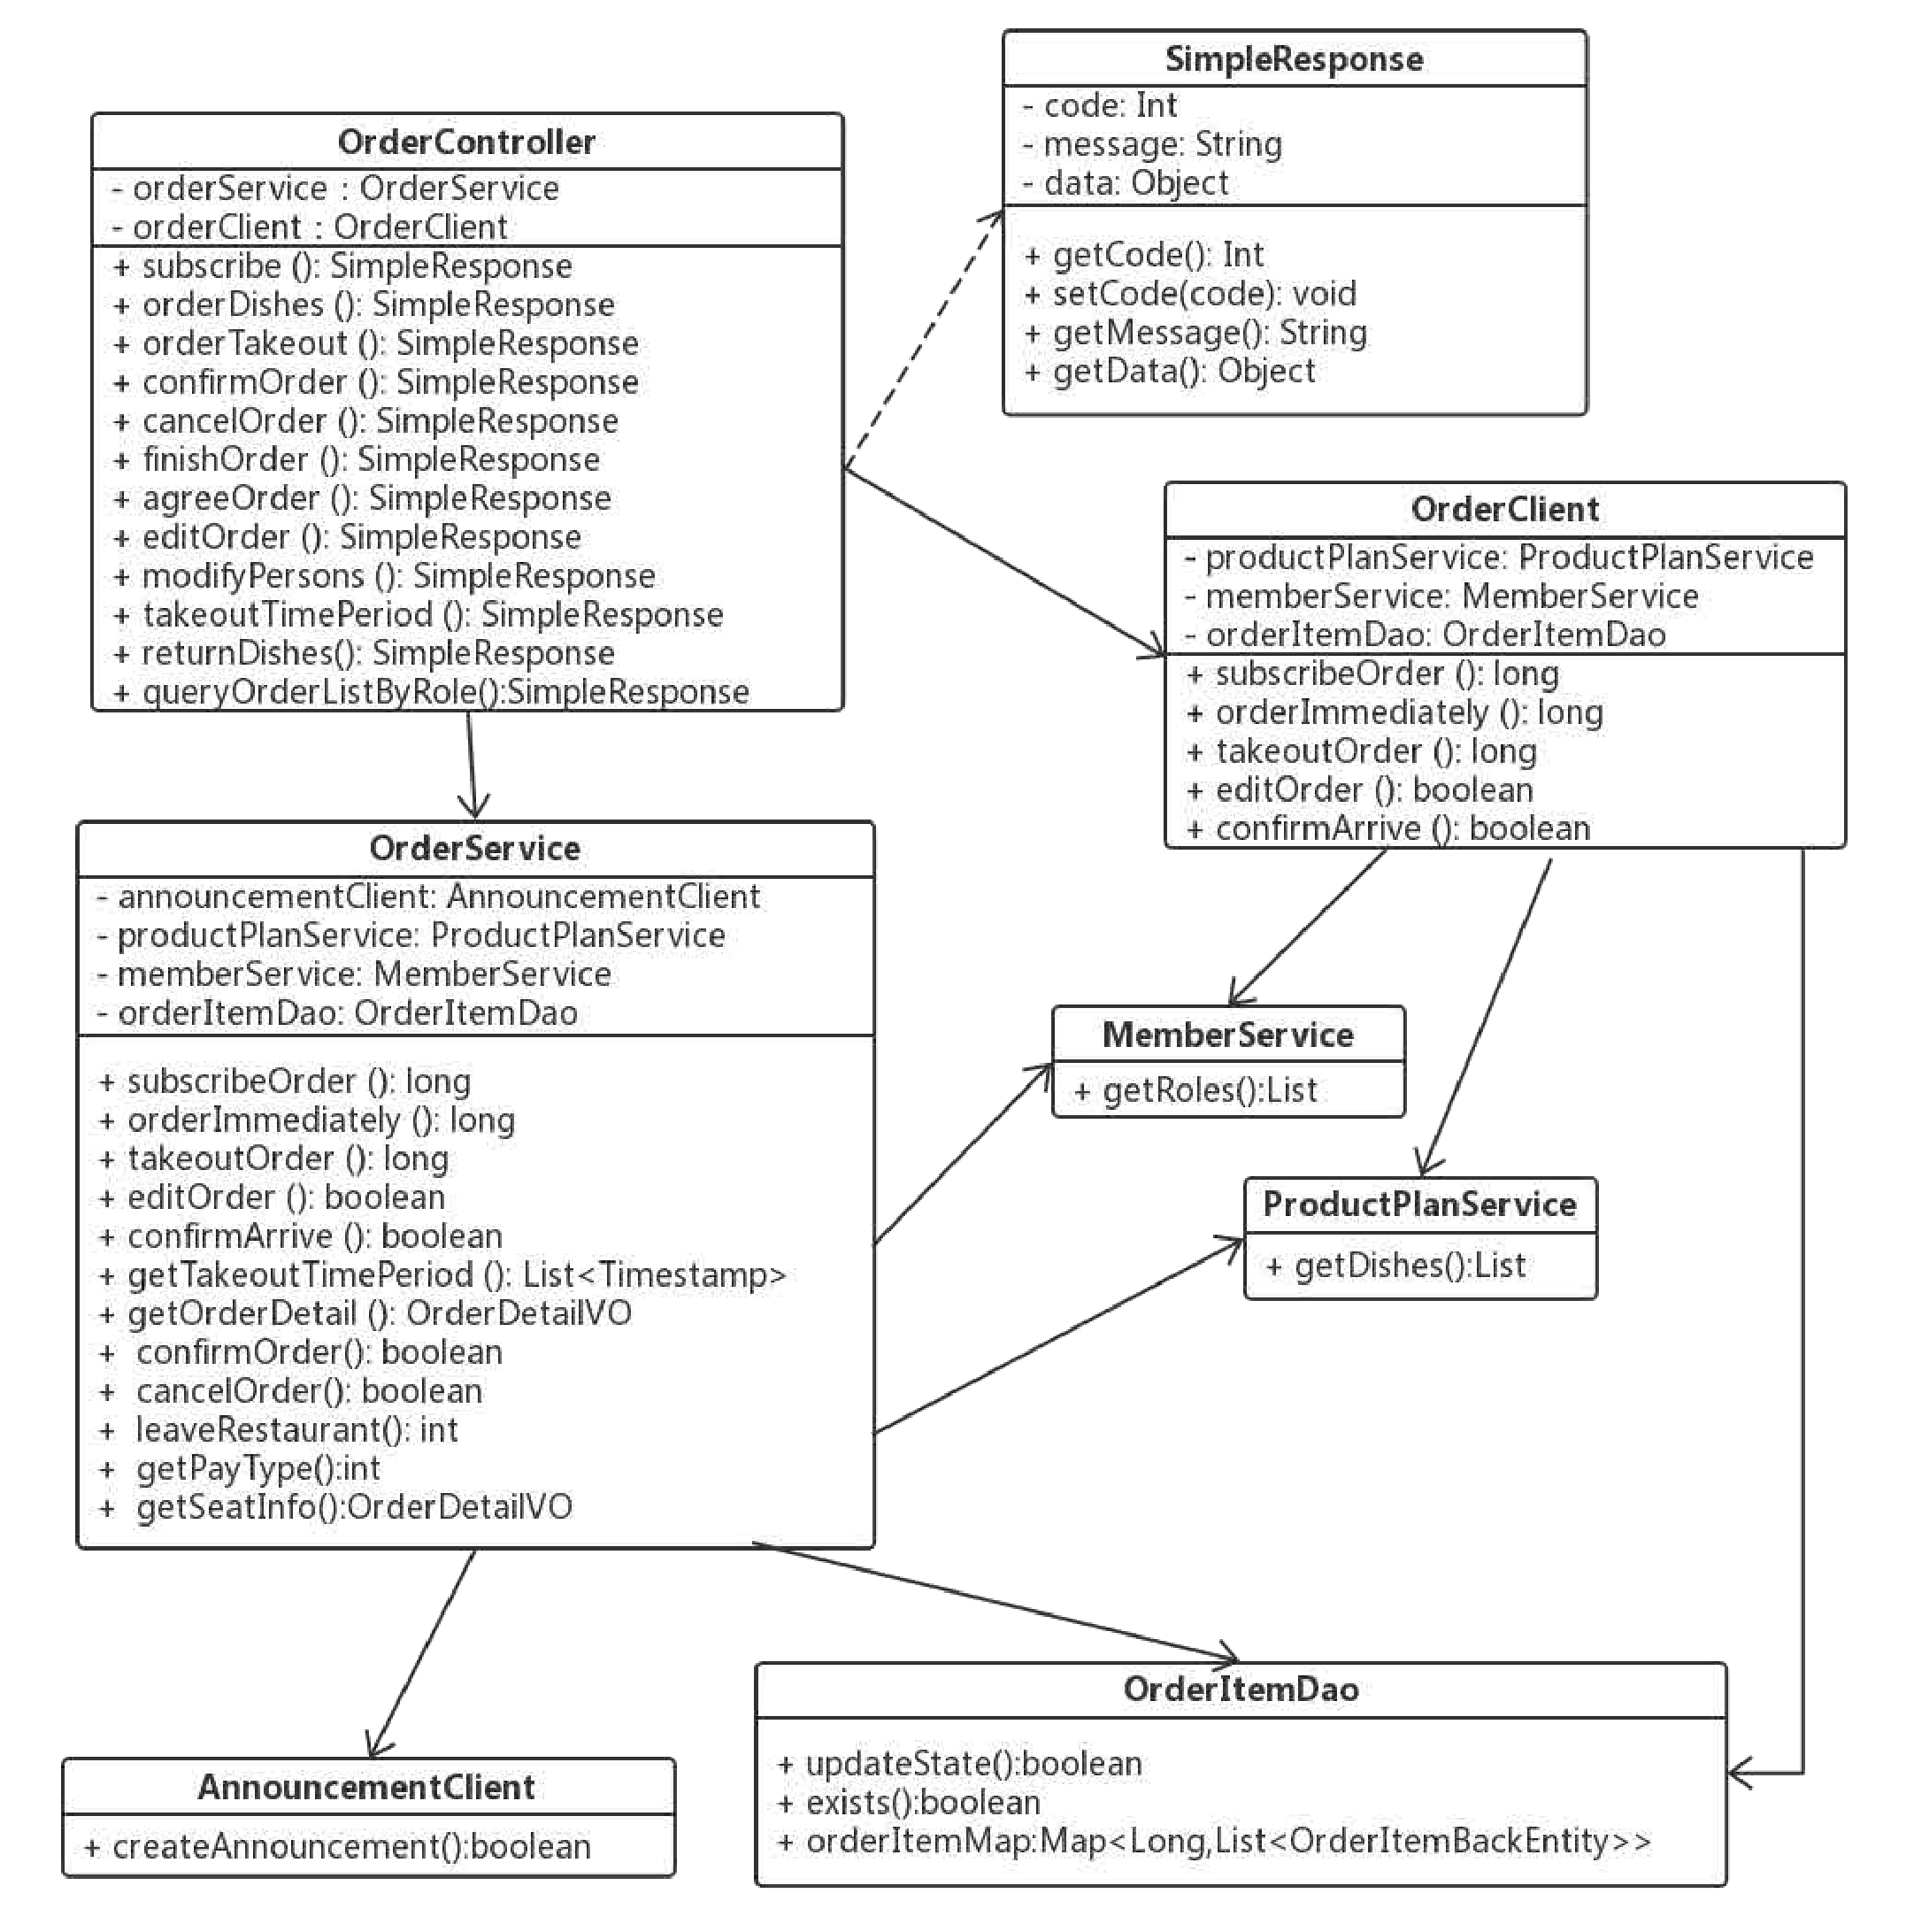
\includegraphics[width=5.2in]{FIGs/chapter4/order.pdf}
    \caption{订单发布模块关键类图}\label{fig_order}
\end{figure}

\begin{table}[htbp!]\footnotesize
    \centering
    \caption{订单发布模块涉及到的类及描述}
    \vspace{2mm}
    \begin{tabular}{clp{0.6\columnwidth}}
    \toprule
    \textbf{序号}&\textbf{名称}&\textbf{描述}\\
    \midrule 
    \textbf{1}& OrderController& 订单控制接口,直接传给前端的数据内容,包括顾客点单以及商家获取、操作订单发布内容。\\
    \hline
    \textbf{2}& OrderService& 订单服务接口,处理订单各类操作,包括提供到店点餐、预约点餐、外卖点餐、编辑订单、确认到店、取消订单等基础操作。\\
    \hline
    \textbf{3}& OrderClient& 订单客户端接口,获取顾客行为,顾客下单后的内容在这里获取。\\
    \hline
    \textbf{4}& SimpleResponse& 简单响应服务,获取接口状态、信息、数据等。\\
    \hline
    \textbf{5}& AnnouncementClient& 发布客户端接口,创建订单发布时需要调用该类创建、编辑等。\\
    \hline
    \textbf{6}& ProductPlanService& 生产计划服务接口,获取菜品详情、库存等内容。\\
    \hline
    \textbf{7}& MemberService& 用户服务接口,这里可以获取用户角色、基本信息、权限等。\\
    \hline
    \textbf{8}& OrderItemDao& 订单条目,更新订单状态、获取订单详情,与数据库交互。\\
    \bottomrule
    \end{tabular}
    \label{table:1List}
\end{table}

如表~\ref{table:1List}所示,订单发布模块主要关联到的java类有OrderController(订单控制接口)、OrderService(订单服务接口)、OrderClient(订单客户端接口)、SimpleResponse(简单响应服务)、AnnouncementClient(发布客户端接口)、ProductPlanService(生产计划服务接口)、MemberService(用户服务接口)、OrderItemDao(订单条目)。\\

\subsection{订单发布模块实现}

\begin{figure}[htbp!]
    \centering
    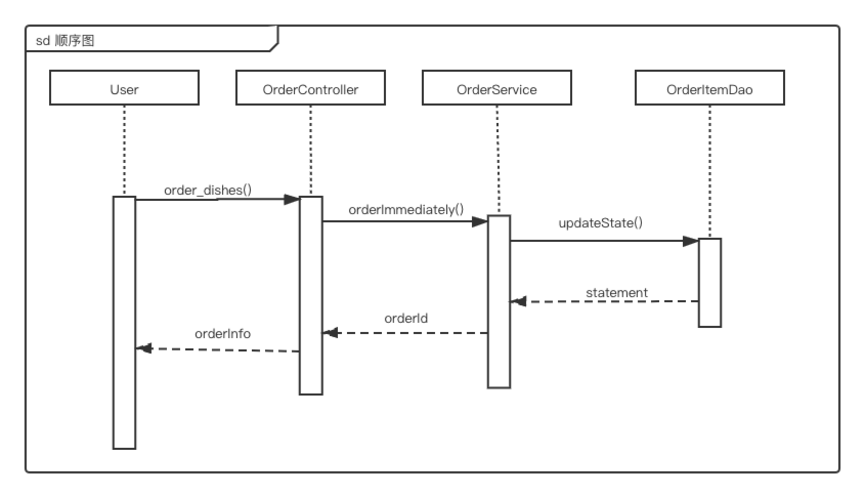
\includegraphics[width=5in]{FIGs/chapter4/order_time.pdf}
    \caption{用户到店点餐的时序图}\label{fig_order_time}
\end{figure}

如图~\ref{fig_order_time}所示,
这是用户到店点餐的过程,用户下单首先会调用OrderController的order\_dishes()方法创建订单,然后会调用OrderService中的orderImmediately()方法创建订单相关内容,在该方法中调用了generateAnnouncementOrder()方法创建订单发布,调用了OrderItemDao类中updateState()方法更新订单发布状态,最终返回给用户订单详情。

这是到店点餐的过程,预约点餐、外卖点餐与之类似,下单后需要根据下单类型创建相应的订单,运行不同任务以及改变其他模块的相关内容。如果是预约点餐,系统会将预约时间段的座位修改为已占用状态,允许用户在规定时间之前取消订单;如果是外卖点餐,系统会提醒商家确认接单,分配骑手送单等。

如图~\ref{fig_order_1}所示是生成订单发布的后端代码,用户下单后,需要在相应的餐厅事务下生成订单,记录其创建时间、公开性、创建内容并生成唯一的发布ID,记录下单用户、下单菜品以及订单状态。创建订单发布的同时调用了OrderClient类的createOrder()方法返回给用户订单详情。

\begin{figure}[htbp!]
    \centering
    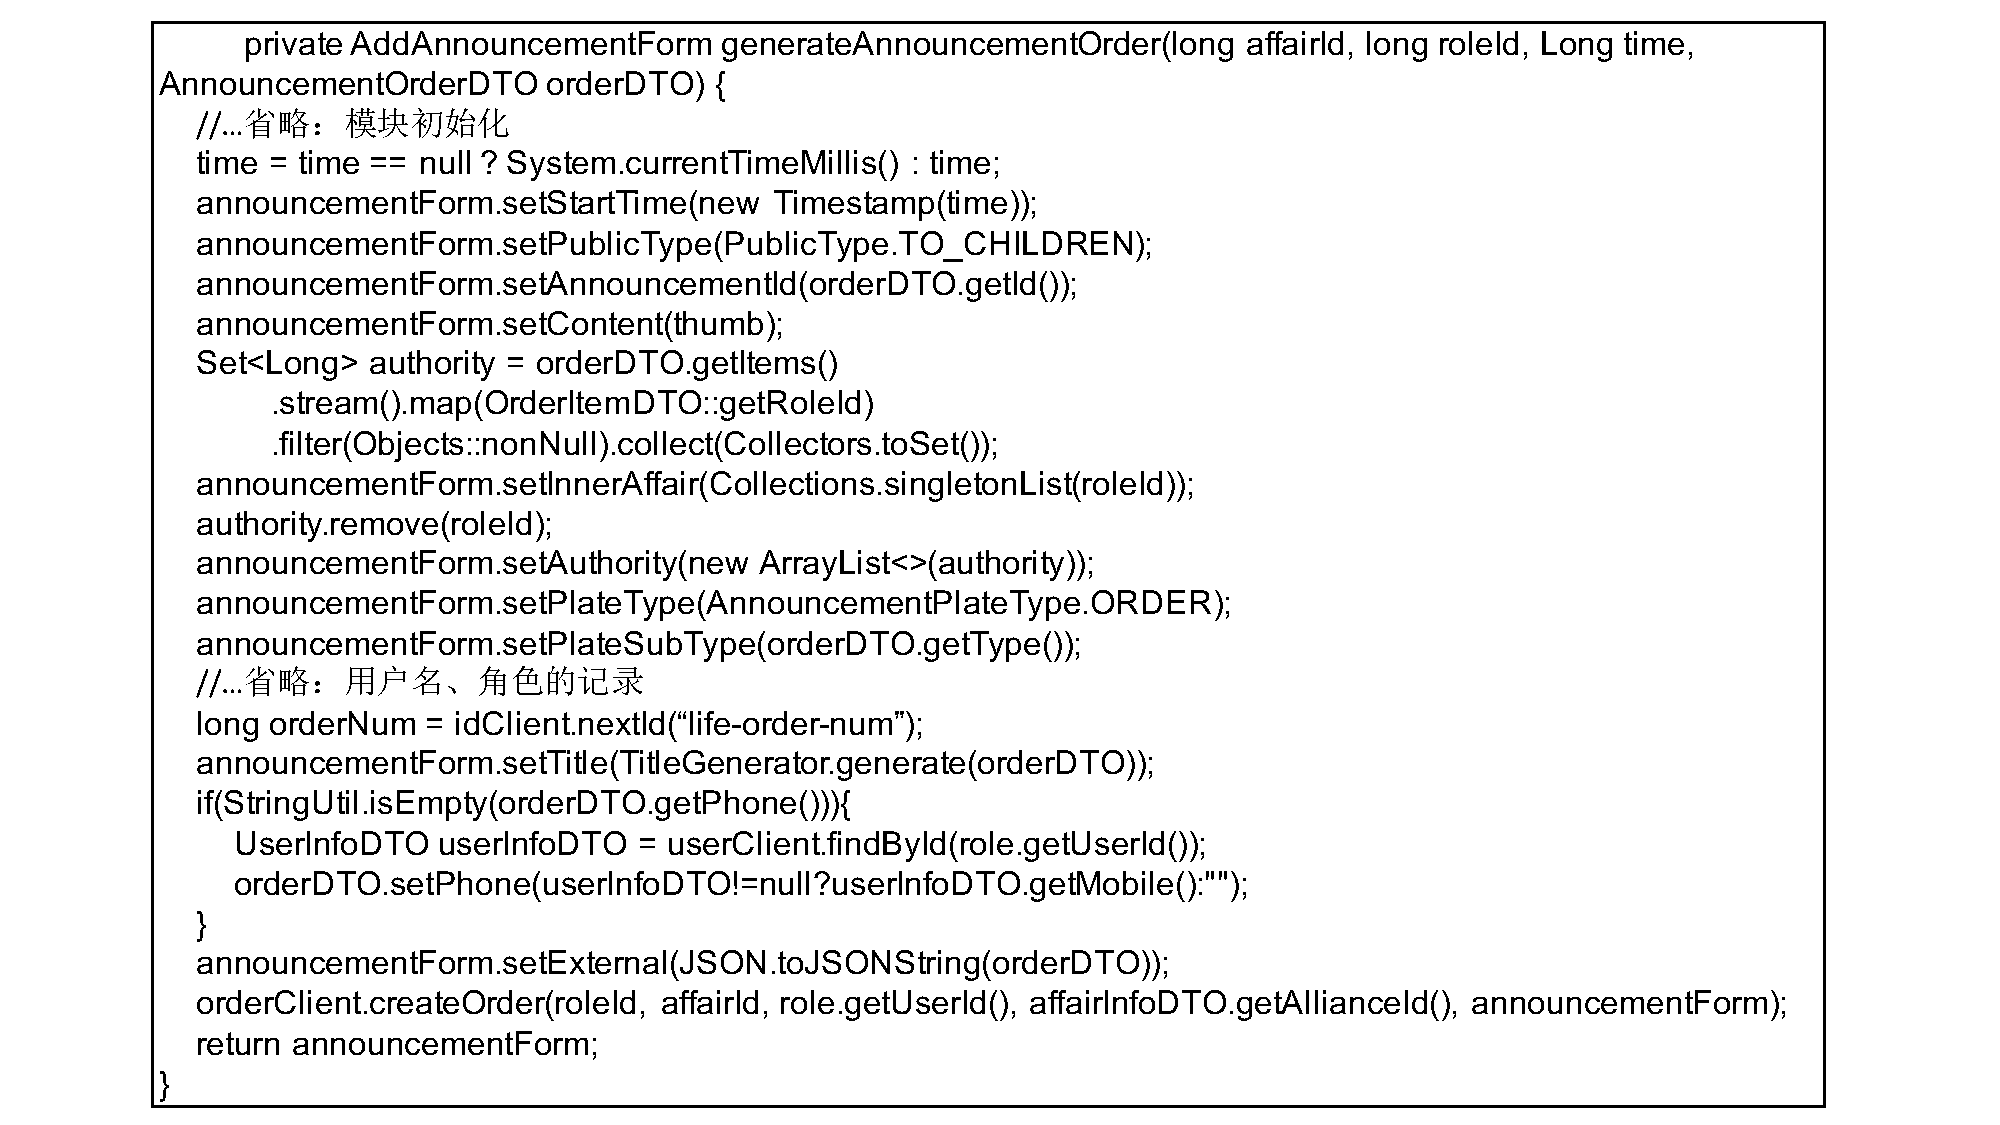
\includegraphics[width=\linewidth]{FIGs/chapter4/1.pdf}
    \caption{生成订单发布代码片段}\label{fig_order_1}
\end{figure}

\begin{figure}[htbp!]
    \centering
    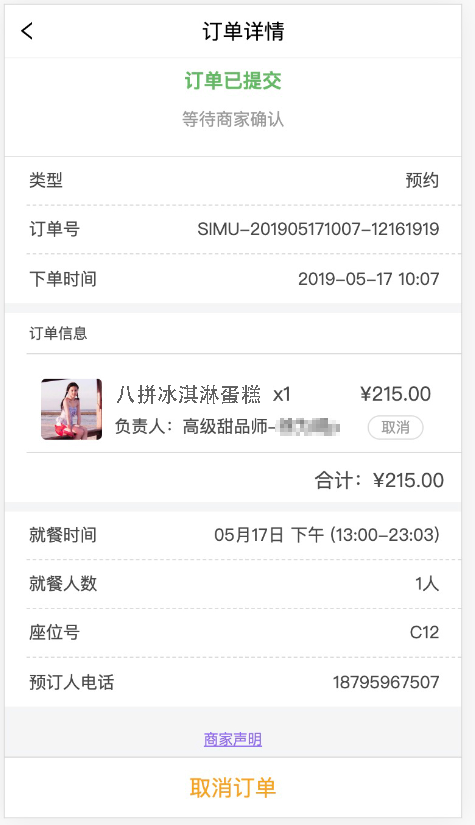
\includegraphics[width=2.5in]{FIGs/chapter4/order_view.pdf}
    \caption{顾客下单后的订单详情}\label{fig_order_view}
\end{figure}

\begin{figure}[htbp!]
    \centering
    \includegraphics[width=\linewidth]{FIGs/chapter4/order_view_all.pdf}
    \caption{订单发布详情和打印订单页面}\label{fig_order_detail}
\end{figure}

如图~\ref{fig_order_view}所示是顾客下单后的订单详情页面,这里以预约类型为例,内容包括订单类型(到店、预约、外卖)、唯一的订单号、下单时间、订单信息(菜品图片、名称、价格、厨师)、菜品合计价格、就餐时间、就餐人数、座位号、预订人电话等信息,顾客可以在商家确认之前取消订单,在菜品上菜之前取消某菜品。

如图~\ref{fig_order_detail}左侧所示是顾客下单后,商家在系统中查看到的相关订单发布的具体内容,这里以到店类型为例,包括订单类型(到店、预约、外卖)、订单名称、订单创建者、更新时间、唯一的订单号、座位号、顾客用餐时间、就餐人数、顾客到店时间、订单详情(产品、数量、总价值、状态、支付状态)、订单总金额等信息。商家可以对就餐人数进行修改,根据顾客需求对菜品做删减,当顾客支付完成后,商家点击确认离店即可完成该订单,还可以根据需要打印订单详情。

点击订单发布标题左侧的打印图标,即可看到如图~\ref{fig_order_detail}右侧所示的要打印订单的详情内容,这里以外卖类型为例,包括餐厅图片、名称、订单号、收货地址、联系电话(会加密保护顾客隐私)、配送时间、配送员、产品(名称、数量、总价值)、订单总金额、优惠金额、实付金额以及商家电话,点击打印即可打印该订单详情页。

% \begin{figure}[htbp!]
%     \centering
%     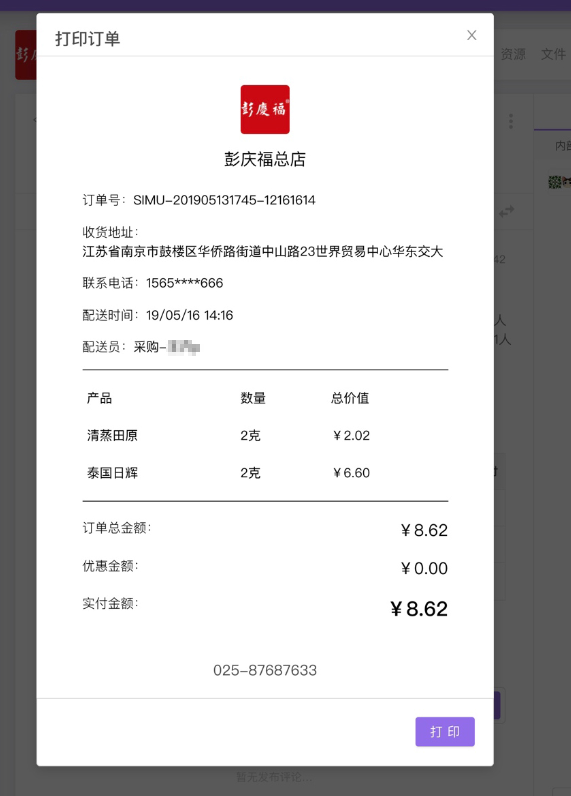
\includegraphics[width=2.5in]{FIGs/chapter4/order_print.pdf}
%     \caption{打印订单}\label{fig_order_print}
% \end{figure}

\section{支付模块}
\subsection{支付模块介绍}
支付模块主要负责处理顾客支付时的支付安全和第三方支付,包括微信支付、支付宝支付等,它依赖于订单发布。对于提交后的订单,顾客支付时系统会调用微信或者支付宝支付接口完成订单支付工作。\\

\subsection{支付模块详细设计}
\begin{figure}[htbp!]
    \centering
    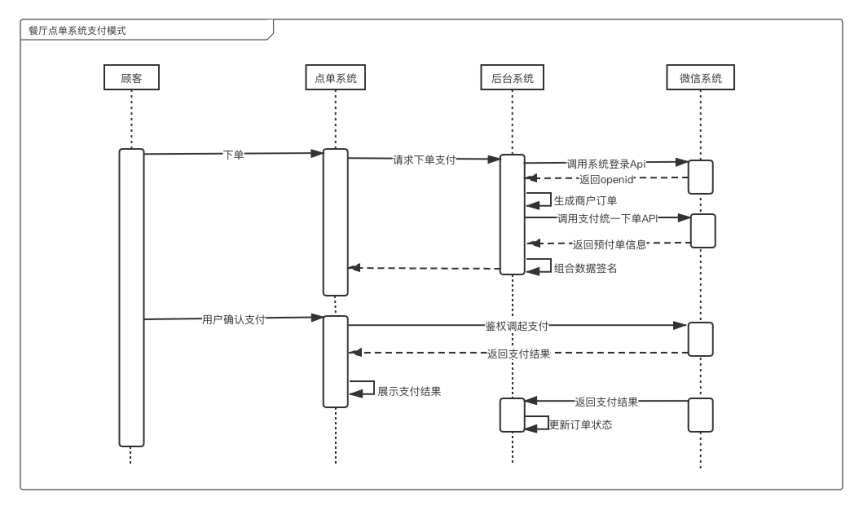
\includegraphics[width=5in]{FIGs/chapter4/pay_time.pdf}
    \caption{点单系统支付模块时序图}\label{fig_pay_time}
\end{figure}

以微信支付为例,微信支付主要分为两种——普通模式和服务商模式,本系统选择普通模式,商家需要申请一个微信公众号绑定店铺,认证通过并且需要成功申请到微信支付功能。此时,商家会在平台中收到唯一的商户号、商户平台密码等内容,可以用于微信支付。开发者可以申请个人的appid以及mch\_id,拥有唯一的appid后可以进行微信公众号内程序的开发,使用微信支付提供给开发者的开放接口来对用户提供相应服务。

微信支付功能的SDK,其中包括WxPay.Api.php(微信支付SDK的接口)、WxPay.Config.php(微信支付的配置文件)、WxPay.Data.php(微信支付中要用到的基本参数对象)、WxPay.Notify.php(接受回调信息的处理类)、WxPay.Exception.php(处理错误异常类)五个主要文件。如图~\ref{fig_pay_time}所示是餐厅点单系统支付模块的时序图,顾客下单后首先会将订单详情发送到后台服务器,由服务器传递参数openid调用微信平台提供的统一下单API,生成预付单并返回到系统的后台服务器,系统将签名后内容和预付单参数信息返还给前端,前端收到信息后调用wx.requestPayment,提交到微信平台,若验证通过则会展示商家的支付二维码界面,顾客扫描二维码即可支付订单。
顾客在公众号内进入系统,选定菜品加入购物车下单。系统生成订单后,会通过wx.navigateTo API跳转到微信的支付模块,调用QRCodePay类实现扫码支付功能,支付成功后微信会返回给顾客相应的支付结果。\\

\subsection{支付模块实现}
\begin{figure}[htbp!]
    \centering
    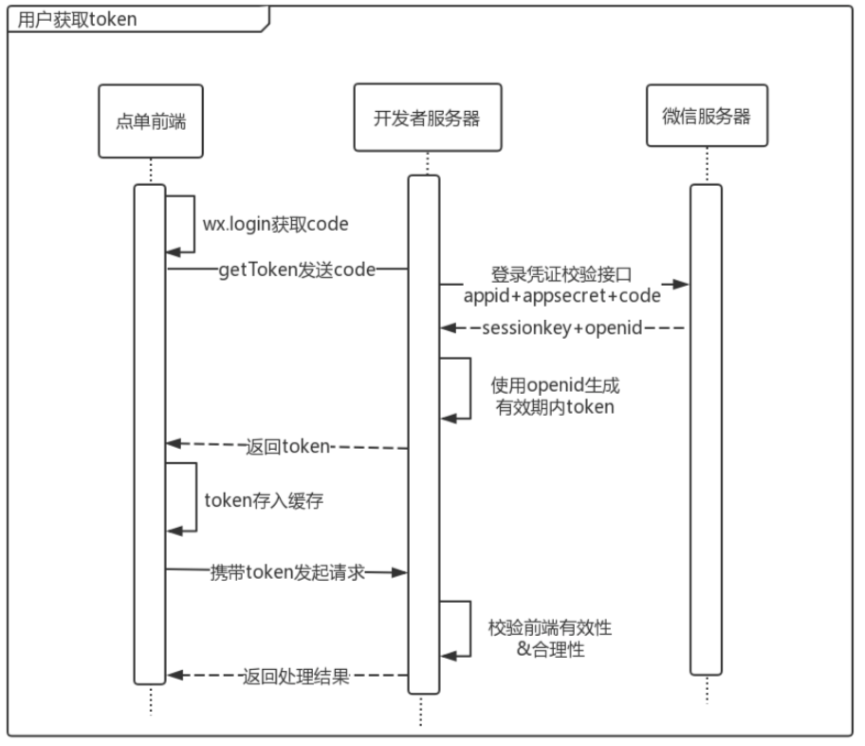
\includegraphics[width=5in]{FIGs/chapter4/pay_token.pdf}
    \caption{用户获取token时序图}\label{fig_pay_token}
\end{figure}

如图~\ref{fig_pay_token}所示,为了验证用户信息,保证支付安全,用户登录时会收到一个code码,后台服务器通过getToken接口把用户信息、code码等内容发送到微信平台中,再由微信平台服务器返回openid以及session\_key参数给后台服务器。
后台服务器需要保存openid,并以此作为验证用户的唯一标志,将其处理加工成一定时间段内有效的token令牌,返回给用户。

用户访问支付接口时,开发者服务器会先对token和openid进行验证,校验通过后,后端会把处理结果返回给前端,用户可以进行相应的后续操作。这样不光保证了支付过程的安全性,而且保护了用户隐私,防止第三方恶意入侵。

\begin{figure}[htbp!]
    \centering
    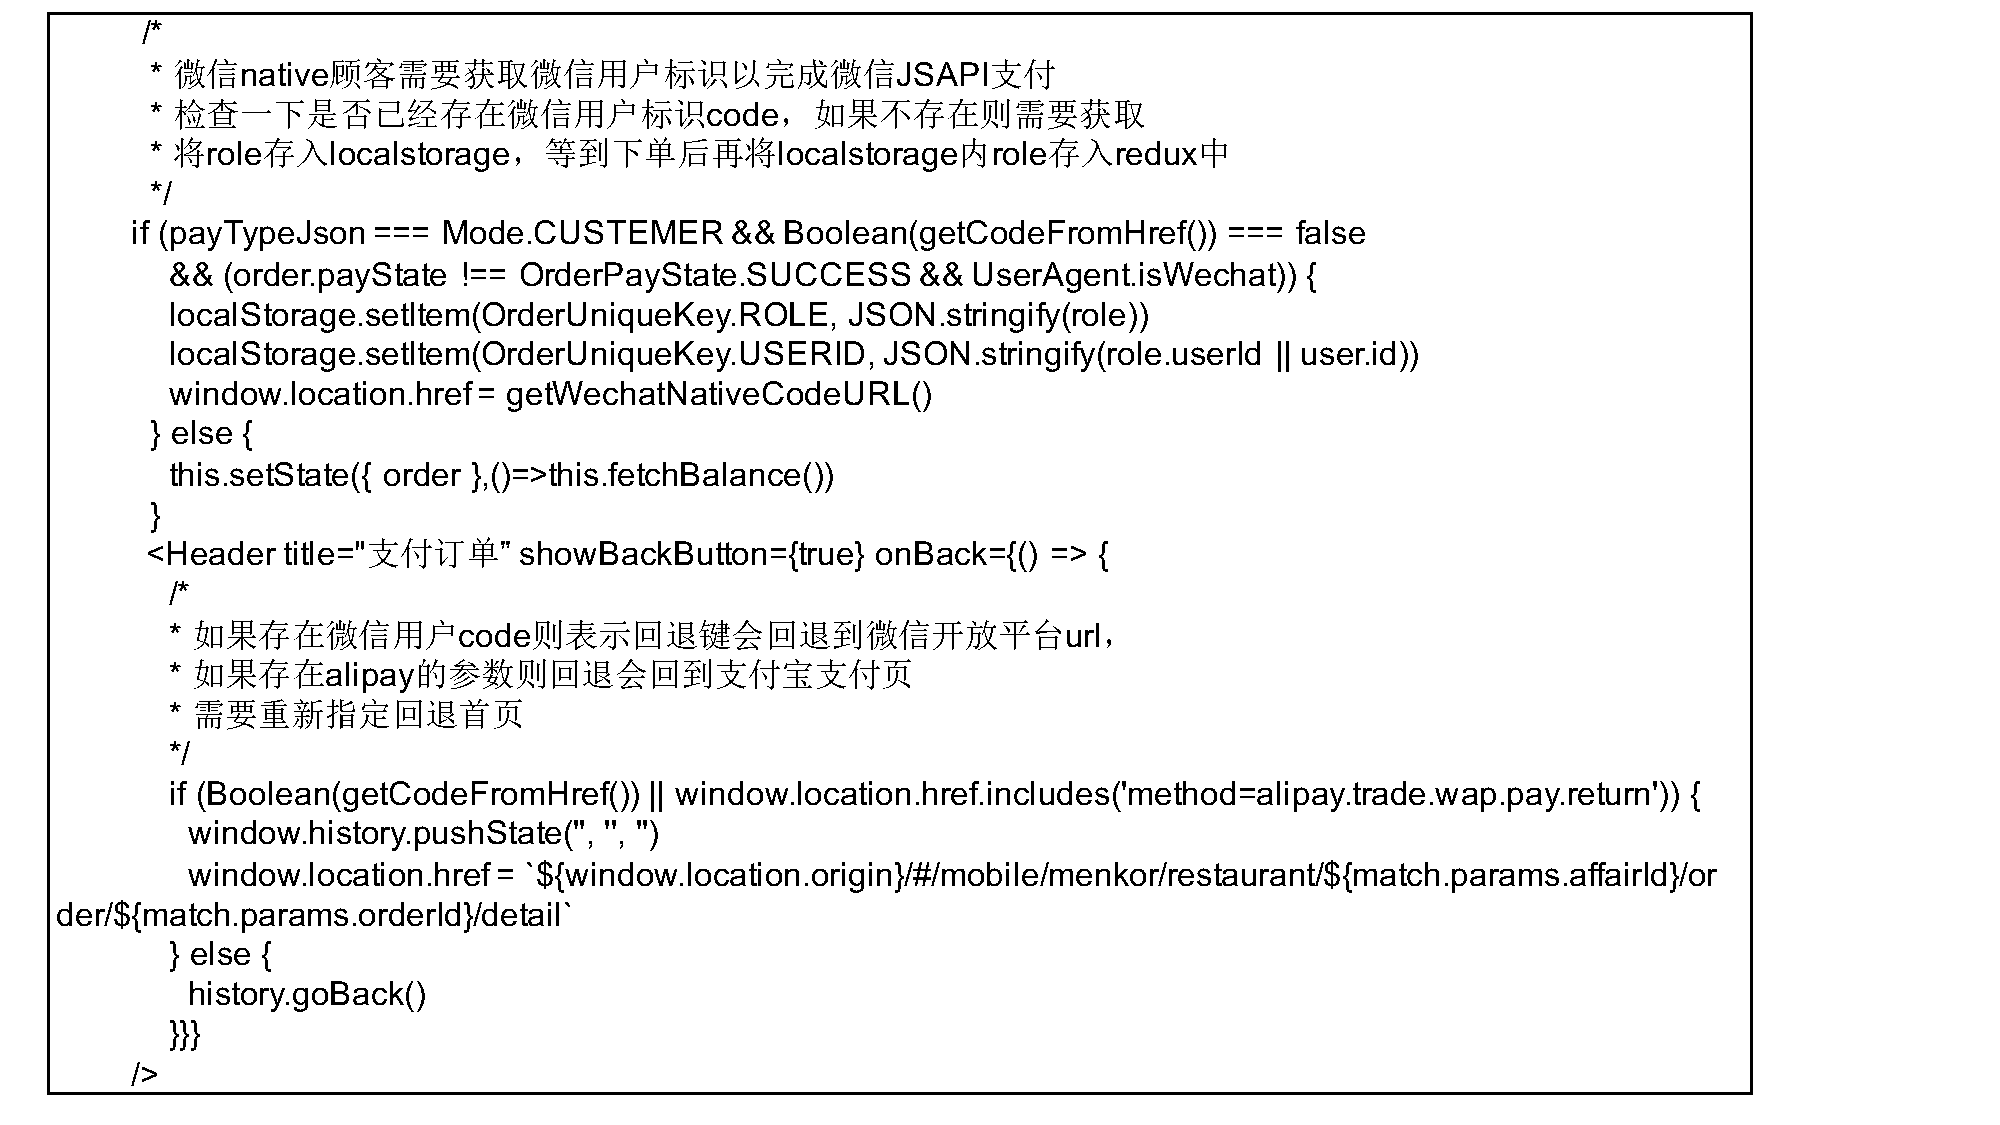
\includegraphics[width=\linewidth]{FIGs/chapter4/2.pdf}
    \caption{判断微信支付代码片段}\label{fig_pay_2}
\end{figure}

系统的线上支付操作一共有两种方式,一种是用户直接点击付款,后端调用相应支付方式的链接以供后续操作;一种是商家出示付款码,用户扫码支付。

如图~\ref{fig_pay_2}所示是前端OrderPaymentContainer订单支付类获取微信用户标识的代码片段,在进入未付款订单前首先判断用户是否为微信用户,如果是则需要获取微信用户标识,如果已经有code码则无须再次获取。系统在回退页上面做了逻辑控制,微信客户端用户与支付宝客户端用户在支付完成后,点击订单界面的返回按钮会回到相对应平台的界面。

为了防止支付完成后,微信刷新页面将缓存内的用户信息清除掉,系统使用了localstorage暂时存储用户信息,等到支付完成后再将其存进Redux的Store内,保持用户数据的实时性与准确性。

支付时同样可以使用商家收款码扫码收款或者现金结账,如图~\ref{fig_pay_3}所示前端ReceiptContainer收款类商家收款代码片段,支持用户使用现金、微信支付、支付宝支付,如果使用现金支付,系统会显示需要支付的金额,商家需要记录抹零后实际收到的金额,保证数据平衡。如果使用微信或者支付宝支付时,系统将返回商家收款码,用户直接扫码即可付款,支付完成3秒后付款码会自动关闭,订单状态更新。

\begin{figure}[htbp!]
    \centering
    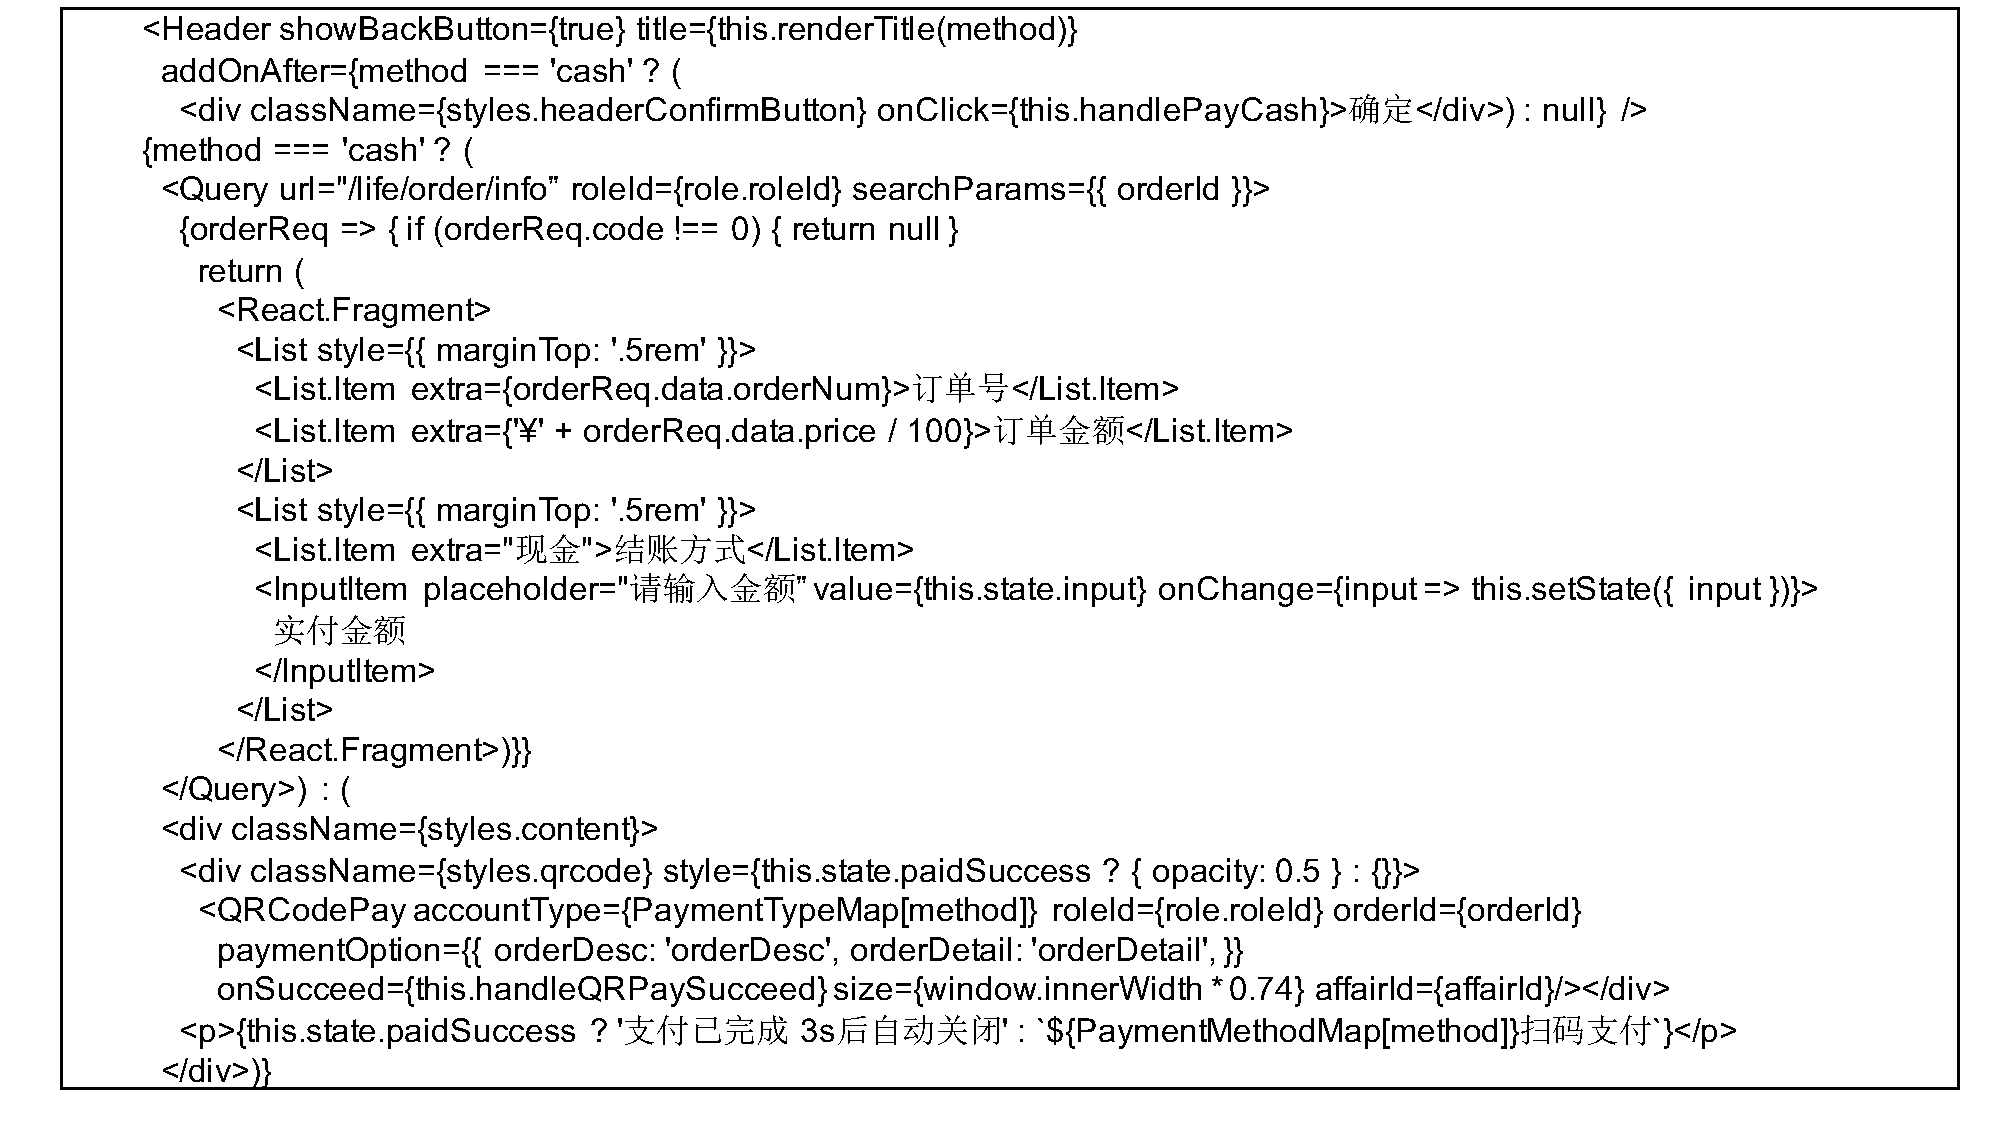
\includegraphics[width=\linewidth]{FIGs/chapter4/3.pdf}
    \caption{商家收款代码片段}\label{fig_pay_3}
\end{figure}

\section{用户管理模块}
\subsection{用户管理模块介绍}
用户管理模块分为两部分:商家部分主要管理餐厅简介、地址、联系电话等信息;顾客部分主要管理账户角色(同一个账号的不同角色可能会对应不同的折扣,使用不同角色登录所看到的订单列表、余额等内容也是不同的)、用户姓名、手机号、配送地址等信息。\\

\subsection{用户管理模块详细设计}
\begin{figure}[htbp!]
    \centering
    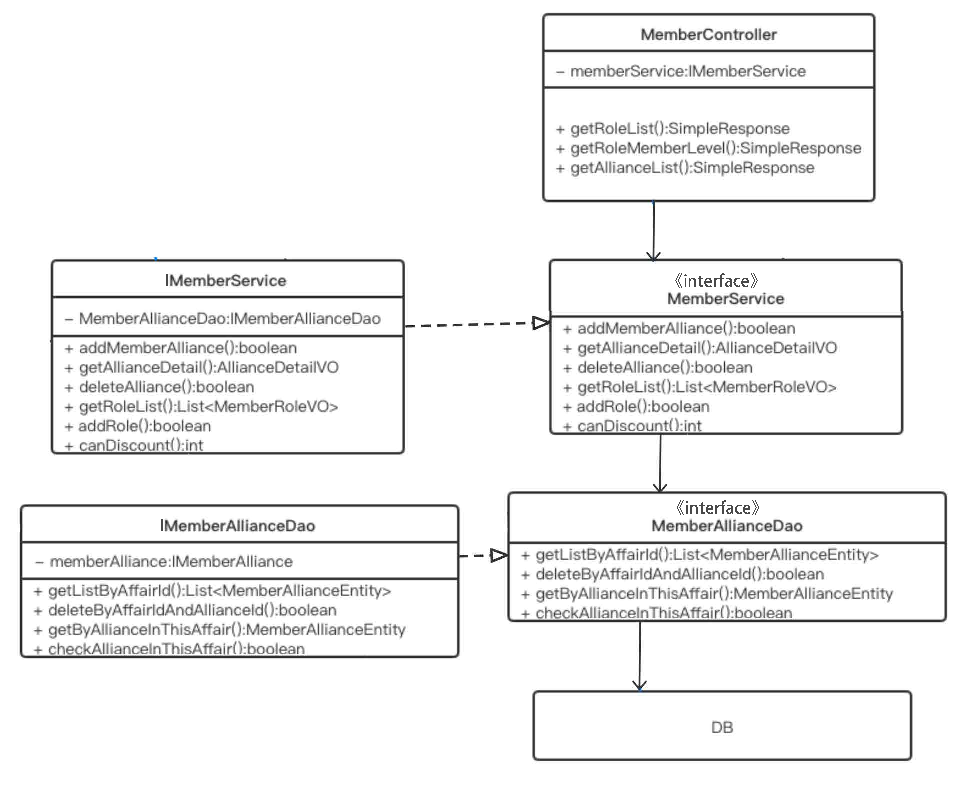
\includegraphics[width=5in]{FIGs/chapter4/user.pdf}
    \caption{用户管理模块类图}\label{fig_user}
\end{figure}

如图~\ref{fig_user}所示是用户管理模块的类图,这里涉及的几个类分别是:
MemberController类是用户控制接口,可以获取用户的角色列表、获取角色会员等级、获取餐厅名称等;MemberService类是用户服务接口,主要提供添加商家店铺、获取餐厅详情、删除餐厅、获取角色列表、判断会员是否享受折扣等服务,其中IMemberService是它的实现类;MemberAllianceDao类是用户服务的Dao层,主要负责与数据库交互,提供基本的用户数据,其中IMemberAllianceDao是它的实现类。

在顾客点单平台中,可以点击用户头像进入到个人中心,查看用户头像、用户名、账号、当前角色等内容。\\

\subsection{用户管理模块实现}
如图~\ref{fig_user_4}是判断顾客当前角色是否享受折扣并且返回相应折扣的方法,顾客所在的分组如果享受折扣,会返回该角色拥有的折扣度,否则直接返回100表示没有折扣。

\begin{figure}[htbp!]
    \centering
    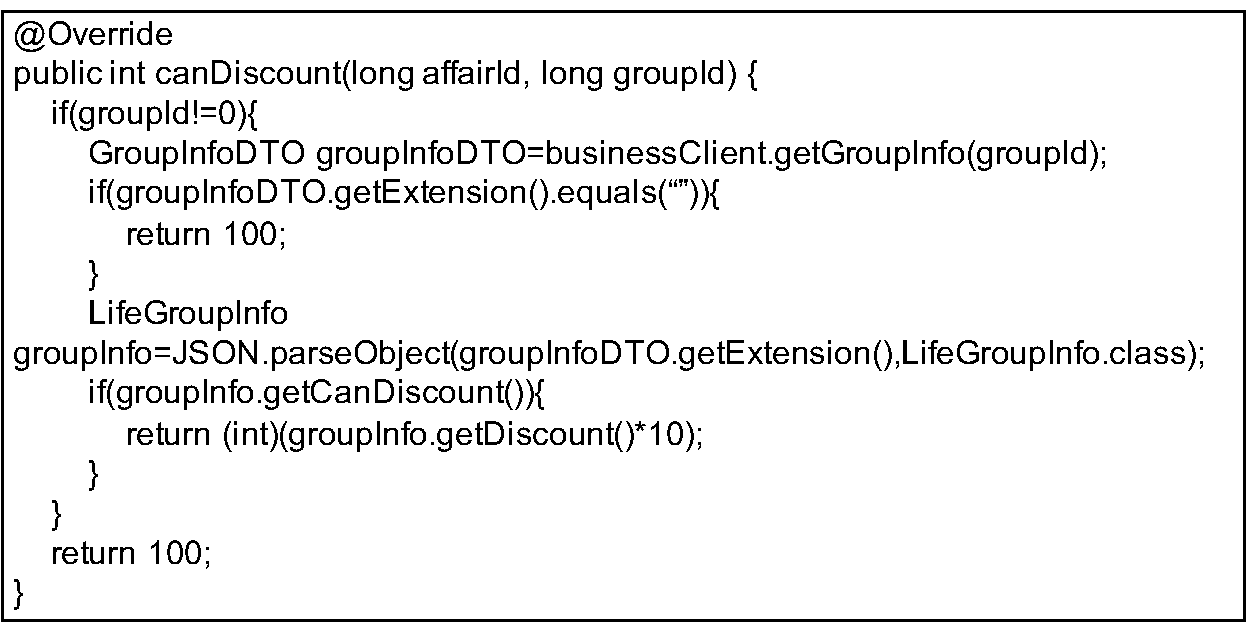
\includegraphics[width=4.2in]{FIGs/chapter4/4.pdf}
    \caption{是否打折的代码片段}\label{fig_user_4}
\end{figure}

如图~\ref{fig_user_5}所示是获取用户所有角色列表的代码片段,通过当前的用户ID与所在餐厅ID去获取当前用户在该餐厅内的所有角色。需要先获取用户的所有角色,再通过餐厅ID筛选当前可选角色,去除重复角色后,将用户本身会员折扣与分组内的会员折扣对比,取最大折扣值返回给相应角色,并按照折扣力度降序排列,返回角色列表。

不同角色拥有不同折扣力度和操作权限。比如一个公司和餐厅达成某种折扣协议,则公司内所有成员角色点单时都享有该力度的折扣;餐厅服务员角色会享受员工折扣,并且有权限代点单,帮助顾客进行下单操作。

\begin{figure}[htbp!]
    \centering
    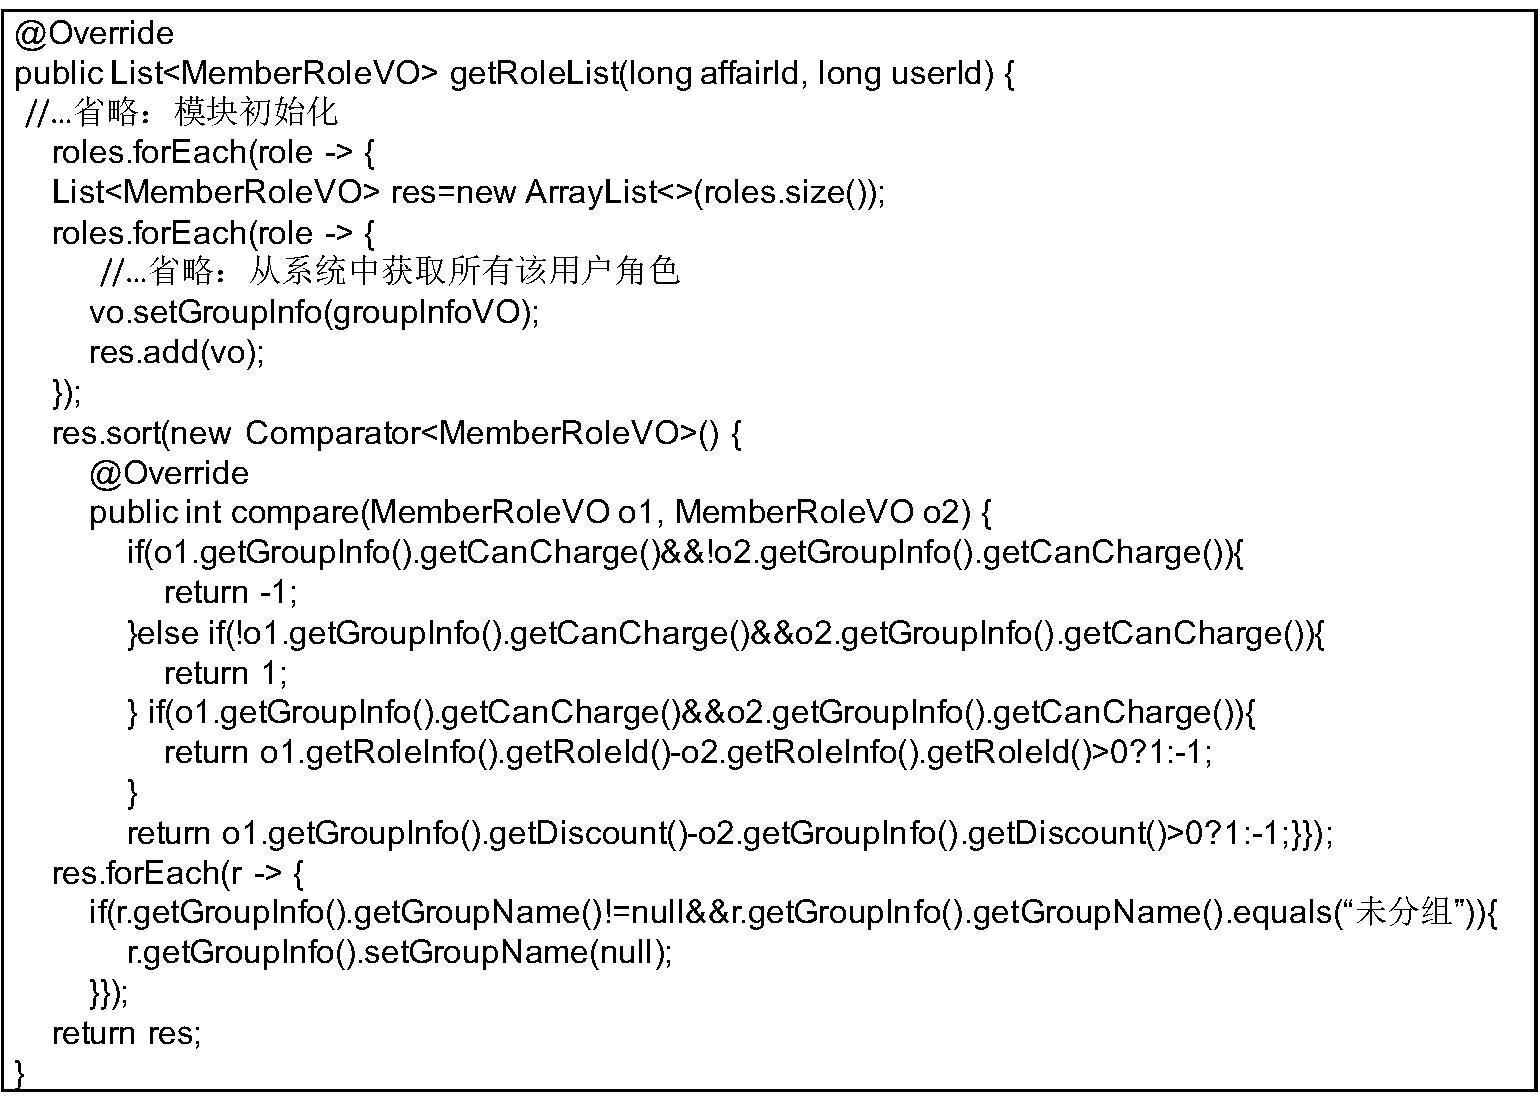
\includegraphics[width=\linewidth]{FIGs/chapter4/5.pdf}
    \caption{获取用户所有的角色列表代码片段}\label{fig_user_5}
\end{figure}

用户登录系统后,可以在如图~\ref{fig_user_role_view}左侧所示的个人中心内,查看当前用户的账户、头像、角色,点击当前角色可以选择切换不同角色。如图~\ref{fig_user_role_view}右侧所示是当前顾客的角色列表(按照会员折扣降序排列),默认角色为最大折扣角色。
顾客有时可能不想自己下单,需要服务员的帮助。餐厅营业员可以登录手机端点单系统,在可选角色列表内选择服务员角色,进行代点单服务。

\begin{figure}[htbp!]
    \centering
    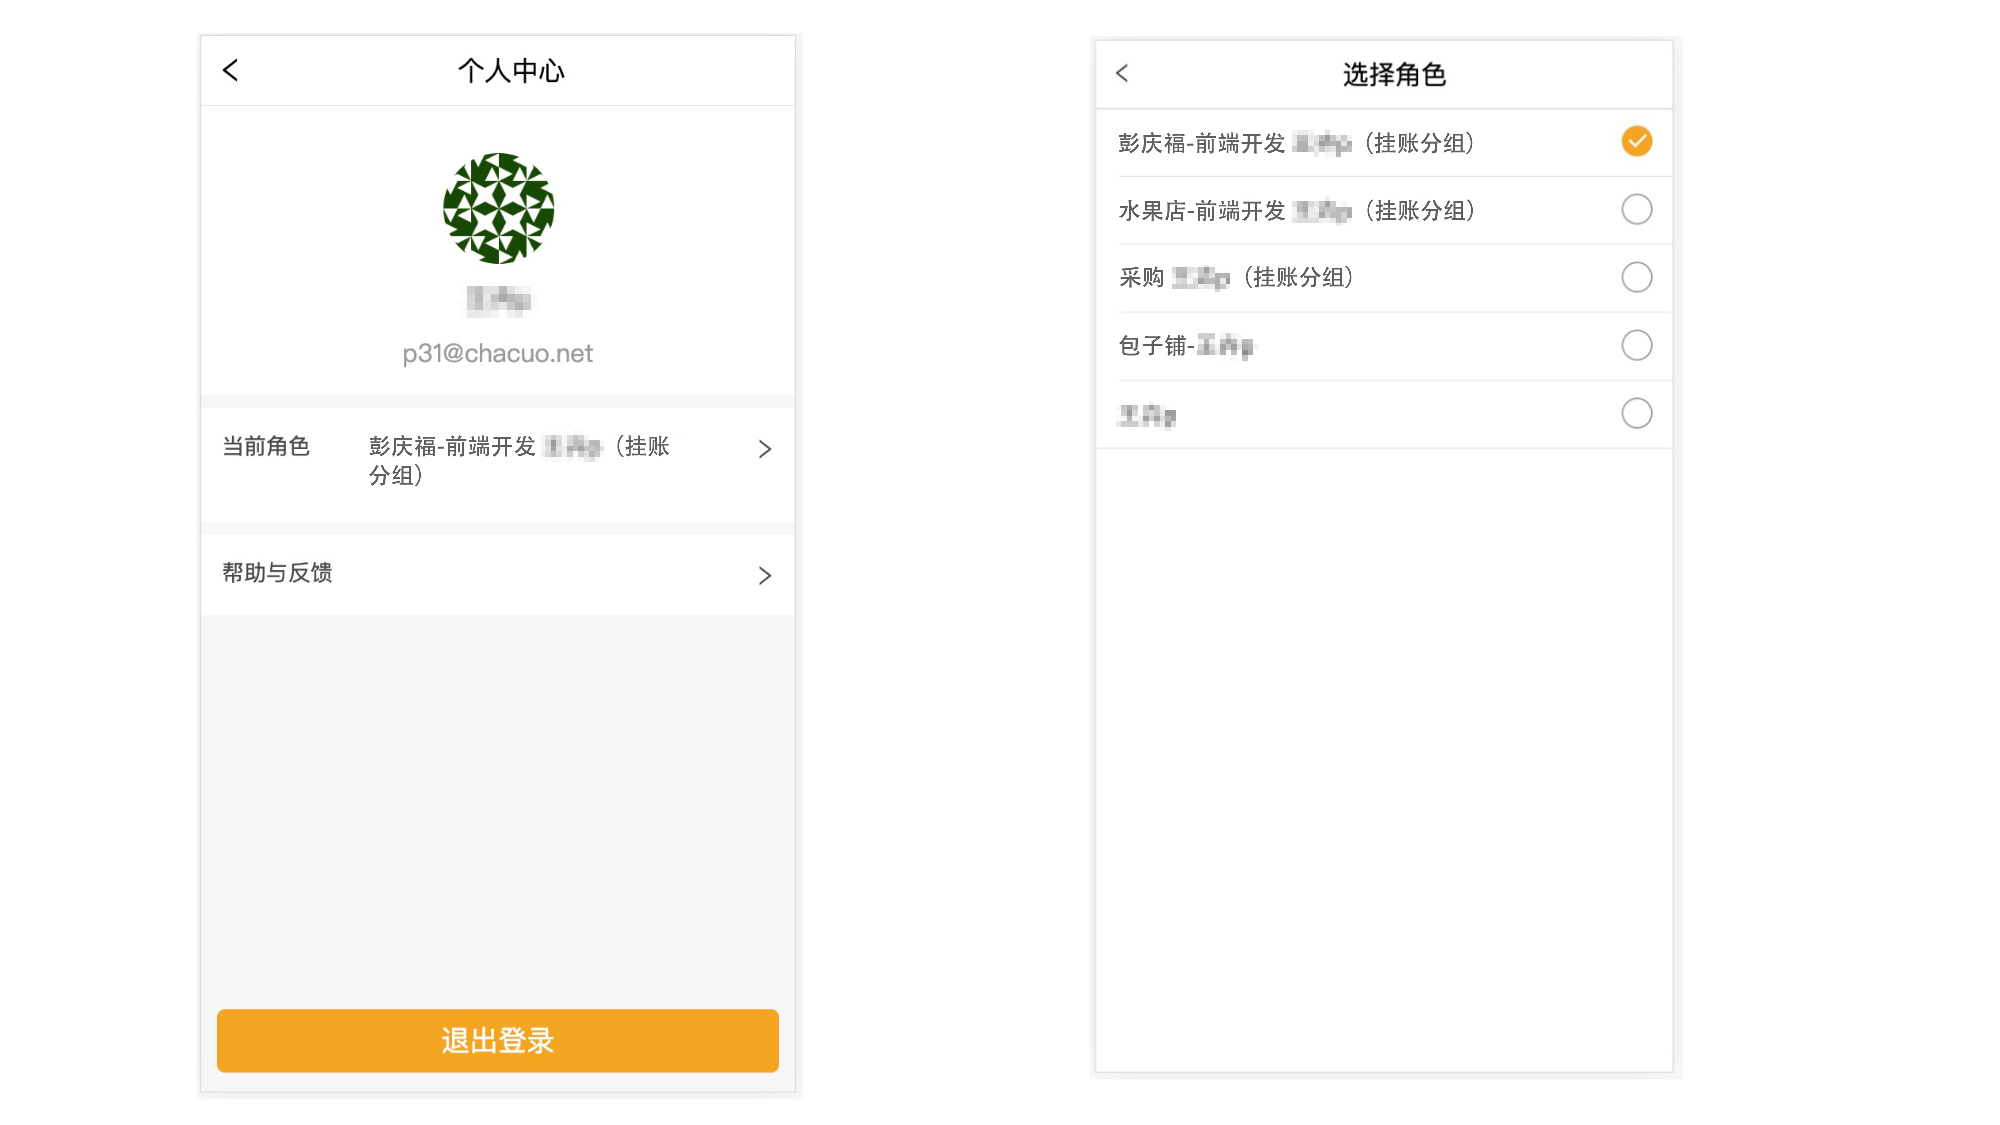
\includegraphics[width=\linewidth]{FIGs/chapter4/user_role_view.pdf}
    \caption{个人中心}\label{fig_user_role_view}
\end{figure}

\section{统计报表模块}
\subsection{统计报表模块介绍}
统计报表模块主要负责收集、整合各报表的信息,对外提供查看日报表、月报表、菜品的进销存日报表、原材料的进销存日报表,下载各报表的服务,为出品发布模块提供下载采购需求的接口。

商家可以在报表内筛选查看每日、每周、每月、每年的菜品统计、销售统计、收支等内容,便于对之后的菜品库存、经营策略、每日配餐组合等内容做出相应调整。\\

\subsection{统计报表模块详细设计}
\begin{figure}[htbp!]
    \centering
    \includegraphics[width=\linewidth]{FIGs/chapter4/table.pdf}
    \caption{统计报表模块类图}\label{fig_table}
\end{figure}

如图~\ref{fig_table}所示是统计报表模块的类图,这里涉及的几个类分别是:ReportFormController类是报表控制接口,可以查看并下载简单报表、复杂日报表、复杂月报表、菜品进销存报表、原材料进销存报表等;ReportFormService类是报表服务接口,主要提供获取简单报表、复杂日报表、复杂月报表等服务,其中IReportFormService是它的实现类;OrderItemDao类前面有介绍过,这里主要用于提供订单详情,其中IOrderItemDao是它的实现类。\\

\subsection{统计报表模块实现}
如图~\ref{fig_table_time}所示是ReportFormController类dailyComplexForm方法的执行时序图,用户点击查看报表,会先调用控制层的查看日报表方法,接着调用ReportFormService类中的getComplexForm方法获取复杂的日报表,这里需要依赖到订单发布模块中OrderItemDao类的orderItemMap方法得到当日订单详情,经过处理返回给上一级,逐步获取、解析并处理好报表信息后,返回报表数据列表给用户。

\begin{figure}[htbp!]
    \centering
    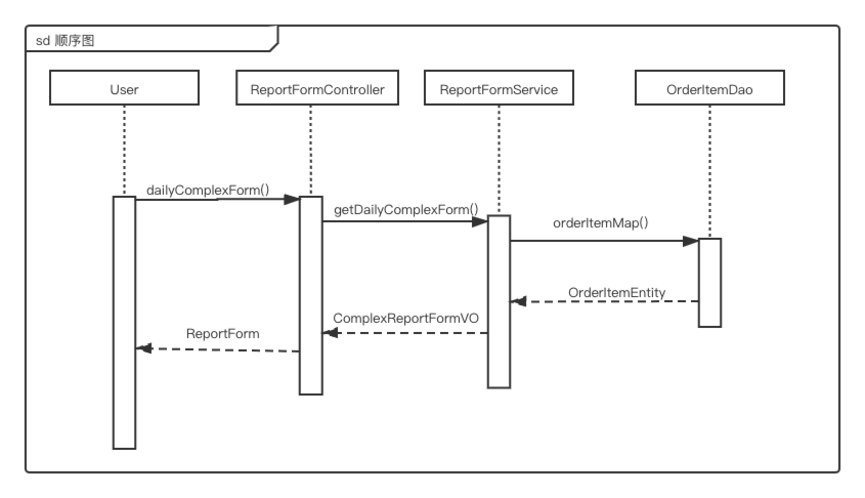
\includegraphics[width=\linewidth]{FIGs/chapter4/table_time.pdf}
    \caption{查看日报表的时序图}\label{fig_table_time}
\end{figure}

\begin{figure}[htbp!]
    \centering
    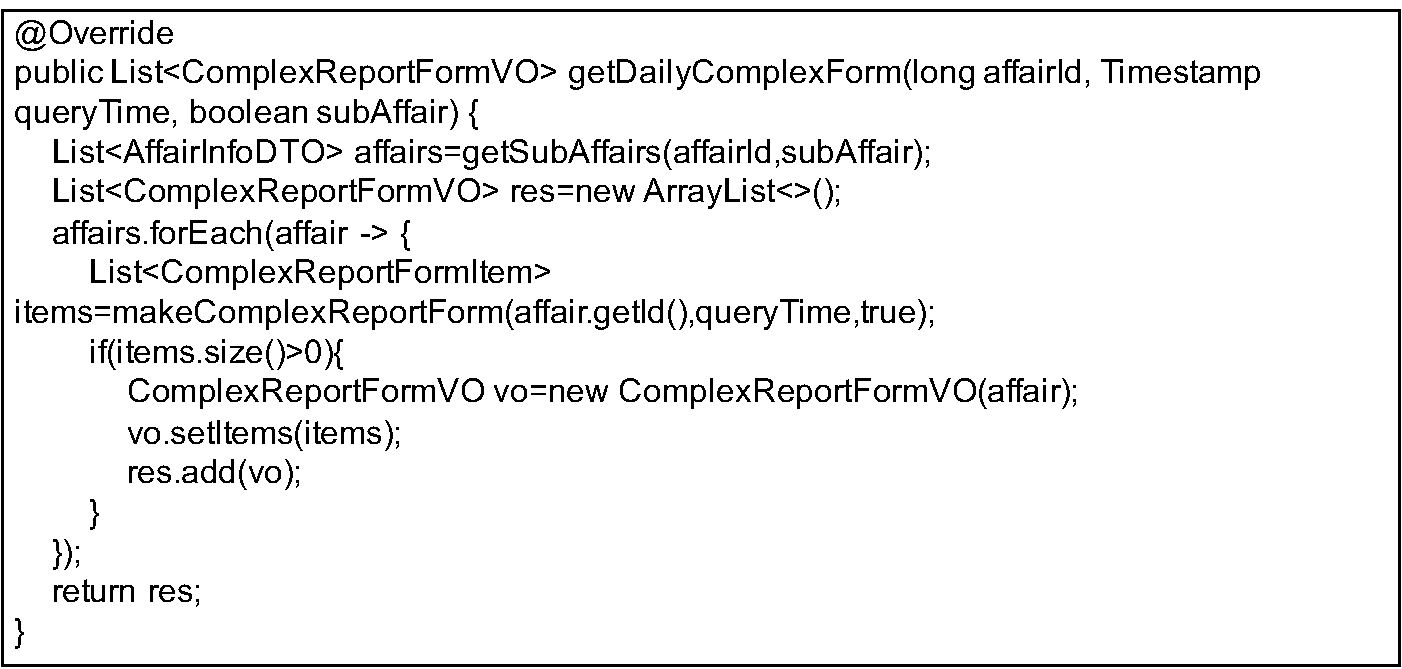
\includegraphics[width=\linewidth]{FIGs/chapter4/6.pdf}
    \caption{ReportFormService类getComplexForm方法代码}\label{fig_table_6}
\end{figure}

统计报表部分实现的代码如图~\ref{fig_table_6}所示,其中调用了私有方法makeComplexReportForm返回报表内容,该方法根据传入的时间参数返回该时间内的报表,根据订单类型(到店、预约、外卖)创建不同的报表内容包括订单折扣、总价、实际收入、支付方式等多种内容~\cite{DBLP:conf/icisa/YangPSC13}。根据传入的餐厅ID来筛选该餐厅下所有的日报表信息(如果该餐厅为连锁餐厅,则可以在总店查看包括总店、分店在内的所有餐厅报表信息)。

\begin{figure}[htbp!]
    \centering
    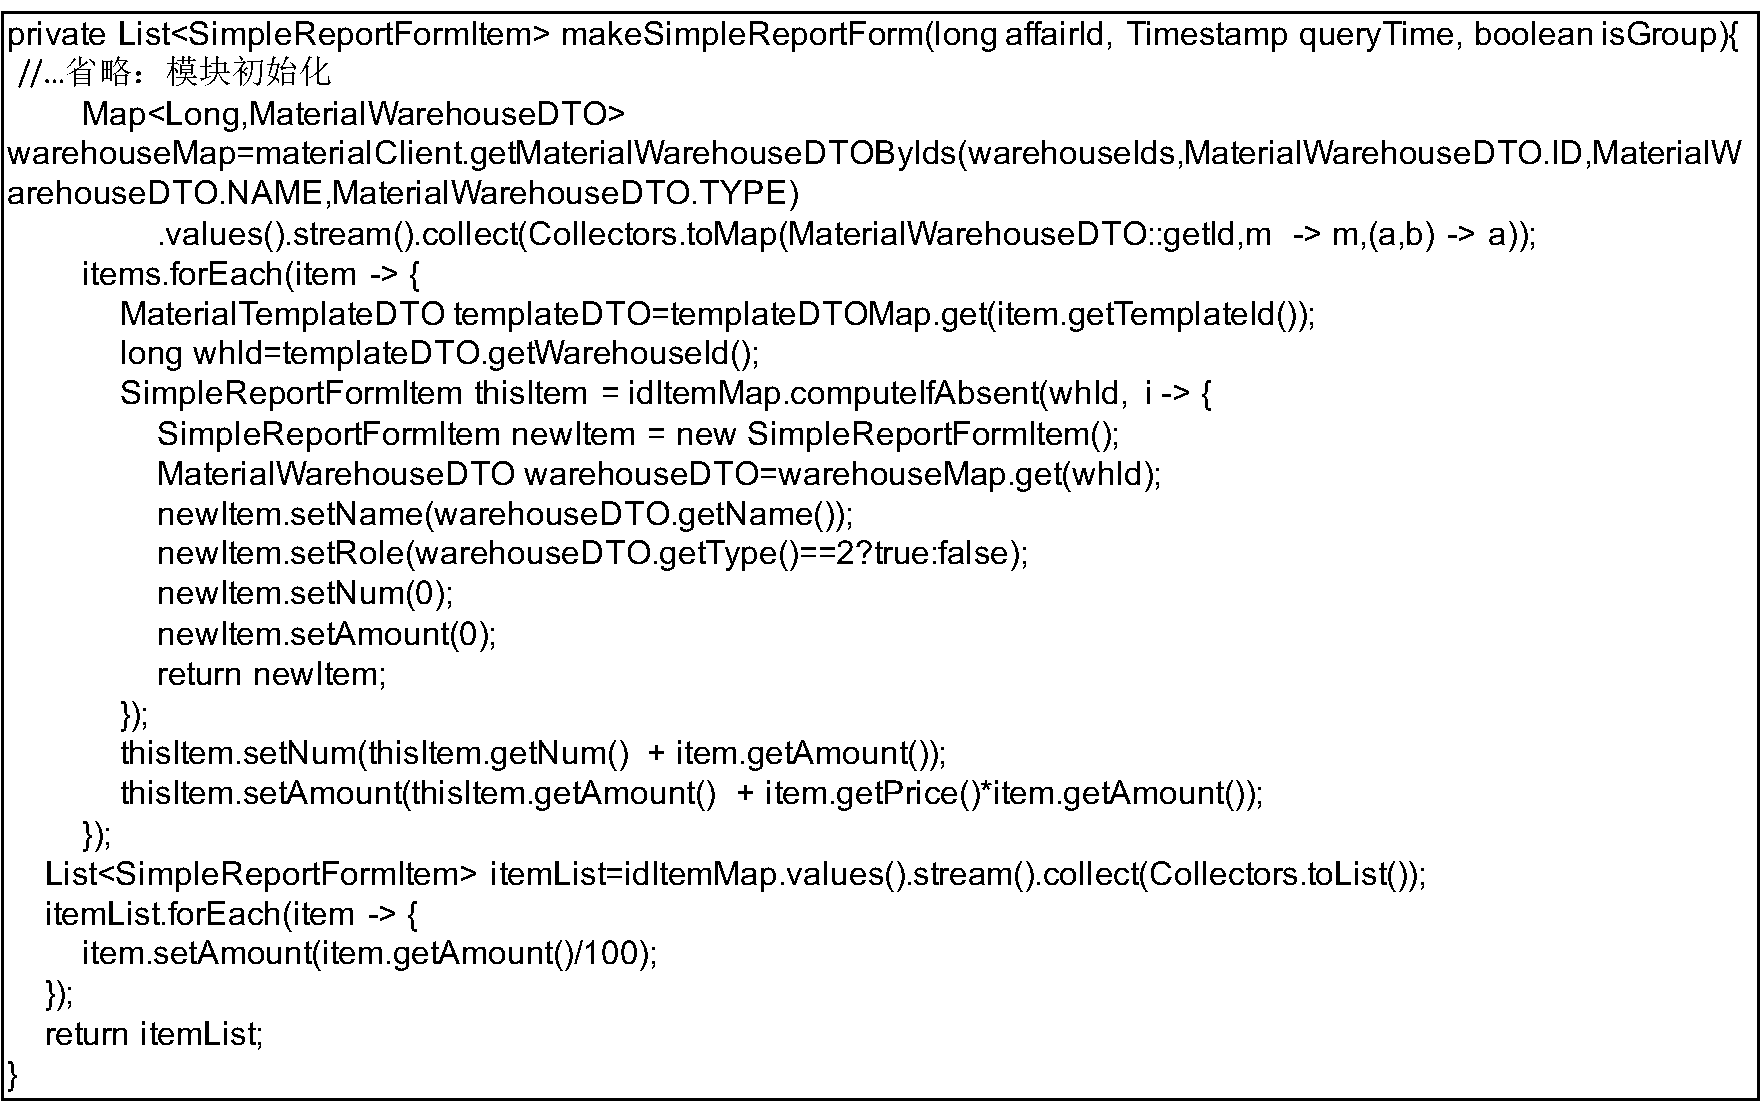
\includegraphics[width=\linewidth]{FIGs/chapter4/7.pdf}
    \caption{ReportFormService类中makeSimpleReportForm方法代码}\label{fig_table_7}
\end{figure}

如图~\ref{fig_table_7}所示是ReportFormService类中makeSimpleReportForm方法的实现代码,该方法用于获取简单报表,不需要区分订单类型,通过传入的日期参数,从餐厅的所有订单列表内筛选相关订单内容,计算订单的总金额,创建多条包括用户名、用户角色、菜品编号、菜品数量、价格等的报表数据,将报表列表返回到Controller层。

用户筛选不同时间段查看统计报表时,前端通过HTTP请求获得返回数据,调用后端接口获取相应时间内的报表内容,进行界面渲染。

\begin{figure}[htbp!]
    \centering
    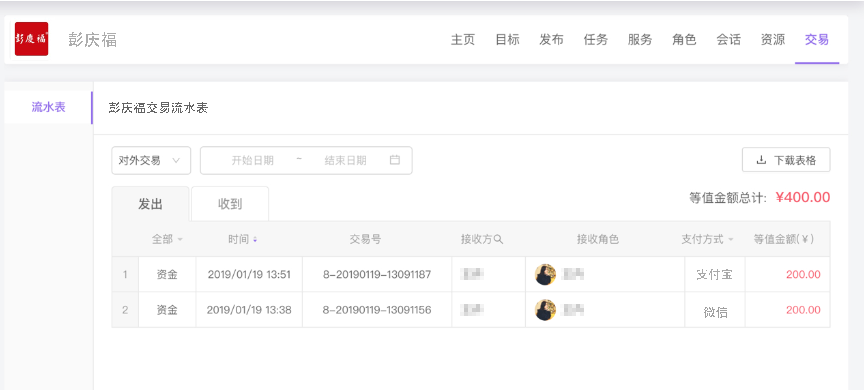
\includegraphics[width=\linewidth]{FIGs/chapter4/table_figure.pdf}
    \caption{简单报表}\label{fig_table_figure}
\end{figure}

如图~\ref{fig_table_figure}所示是简单报表的前端界面,可以根据交易类型、起止时间来筛选查看不同的报表内容,报表内容主要包括类型、时间、交易号、接收方信息、支付方式以及金额等内容,可以点击下载表格将报表内容存储到本地。

\section{座位管理模块}
\subsection{座位管理模块介绍}
座位管理模块主要处理与座位库以及座位有关的操作,对外提供管理座位库的平面视角、卡片视角以及时间轴视角,对座位进行增删改查、更改座位状态、检查是否有重名座位、获取座位信息、座位二维码、座位状态等接口,同时还负责向订单发布模块提供与订单绑定的座位信息等接口。\\

\subsection{座位管理模块详细设计}
\begin{figure}[htbp!]
    \centering
    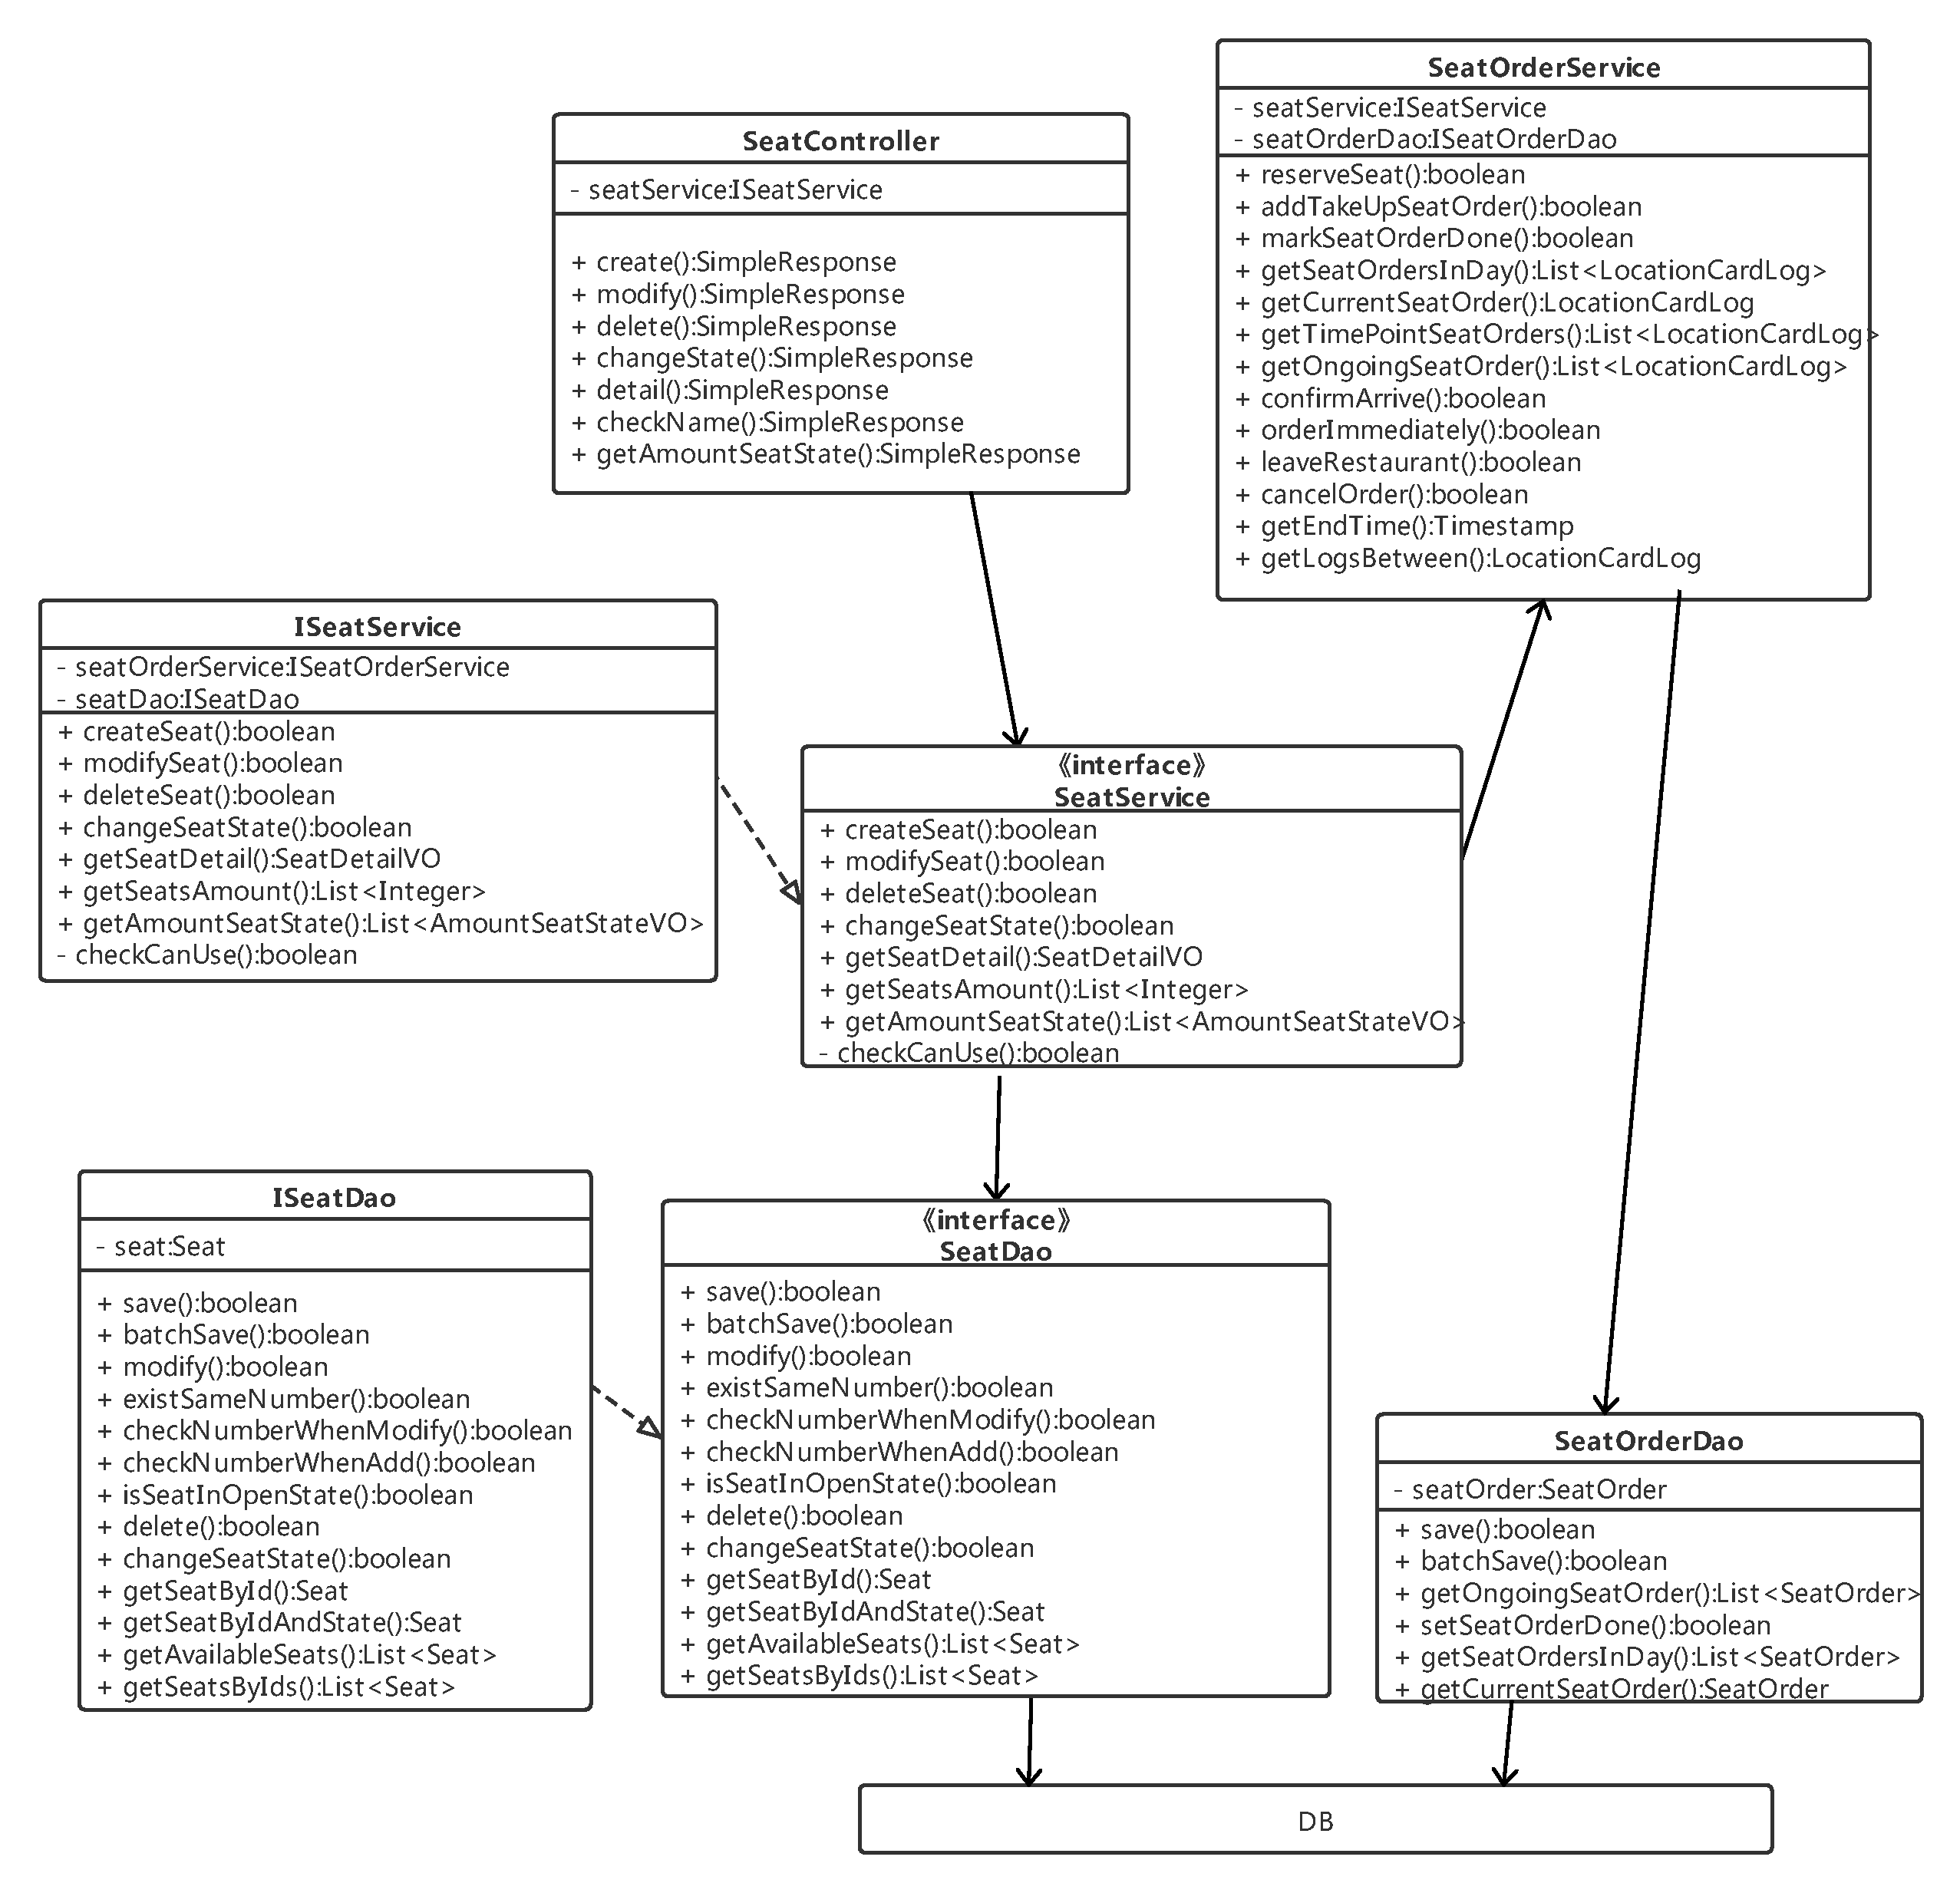
\includegraphics[width=\linewidth]{FIGs/chapter4/seat.pdf}
    \caption{座位管理模块类图}\label{fig_seat}
\end{figure}

如图~\ref{fig_seat}所示是座位管理模块的类图,这里涉及的几个类分别是:

SeatController类是座位控制接口,可以查看三种视图的座位列表,创建、修改、删除座位,修改座位状态,查看座位详情,检查座位名称是否重复,获取可用座位数量等。

SeatService类是座位管理服务接口,主要提供增删改查座位、获取座位数量、获取座位详情、获取可用座位数量、更改座位状态等服务,其中ISeatService是它的实现类。

SeatOrderService类是座位订单管理服务接口,主要提供预订座位、增加占用座位订单、标记座位订单完成、获取某座位当前记录、获取时间点座位列表、获取座位使用记录、确认到店、获取时间段内座位日志等服务。

SeatDao主要用于提供座位增删改查、检索名称是否有重复、座位是否为开放状态等基本操作,其中ISeatDao是它的实现类。

SeatOrderDao主要提供座位订单的相关基本操作,比如标记座位订单完成、获取正在进行的座位订单、获取当天的座位被调用详情、获取当前时间点座位记录等,其中ISeatOrderDao是它的实现类。\\

\subsection{座位管理模块实现}
\begin{figure}[htbp!]
    \centering
    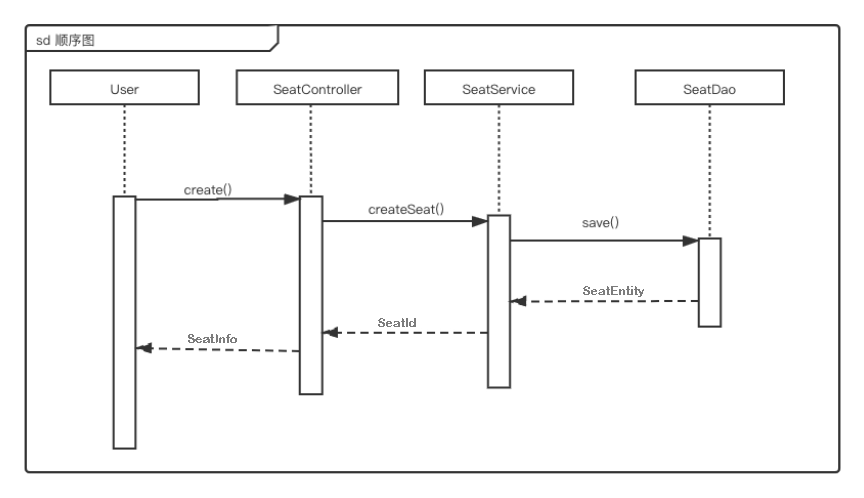
\includegraphics[width=5in]{FIGs/chapter4/seat_time.pdf}
    \caption{创建座位的时序图}\label{fig_seat_time}
\end{figure}

如图~\ref{fig_seat_time}所示是SeatController类create方法的执行时序图,用户点击创建座位,填写完内容点击创建会调用SeatService类中的createSeat方法,进而调用SeatDao的save将座位内容保存到数据库中。座位创建完成后会返回success信息给前端,再重新调用获取座位列表的接口来更新座位列表的界面,显示最新内容。

\begin{figure}[htbp!]
    \centering
    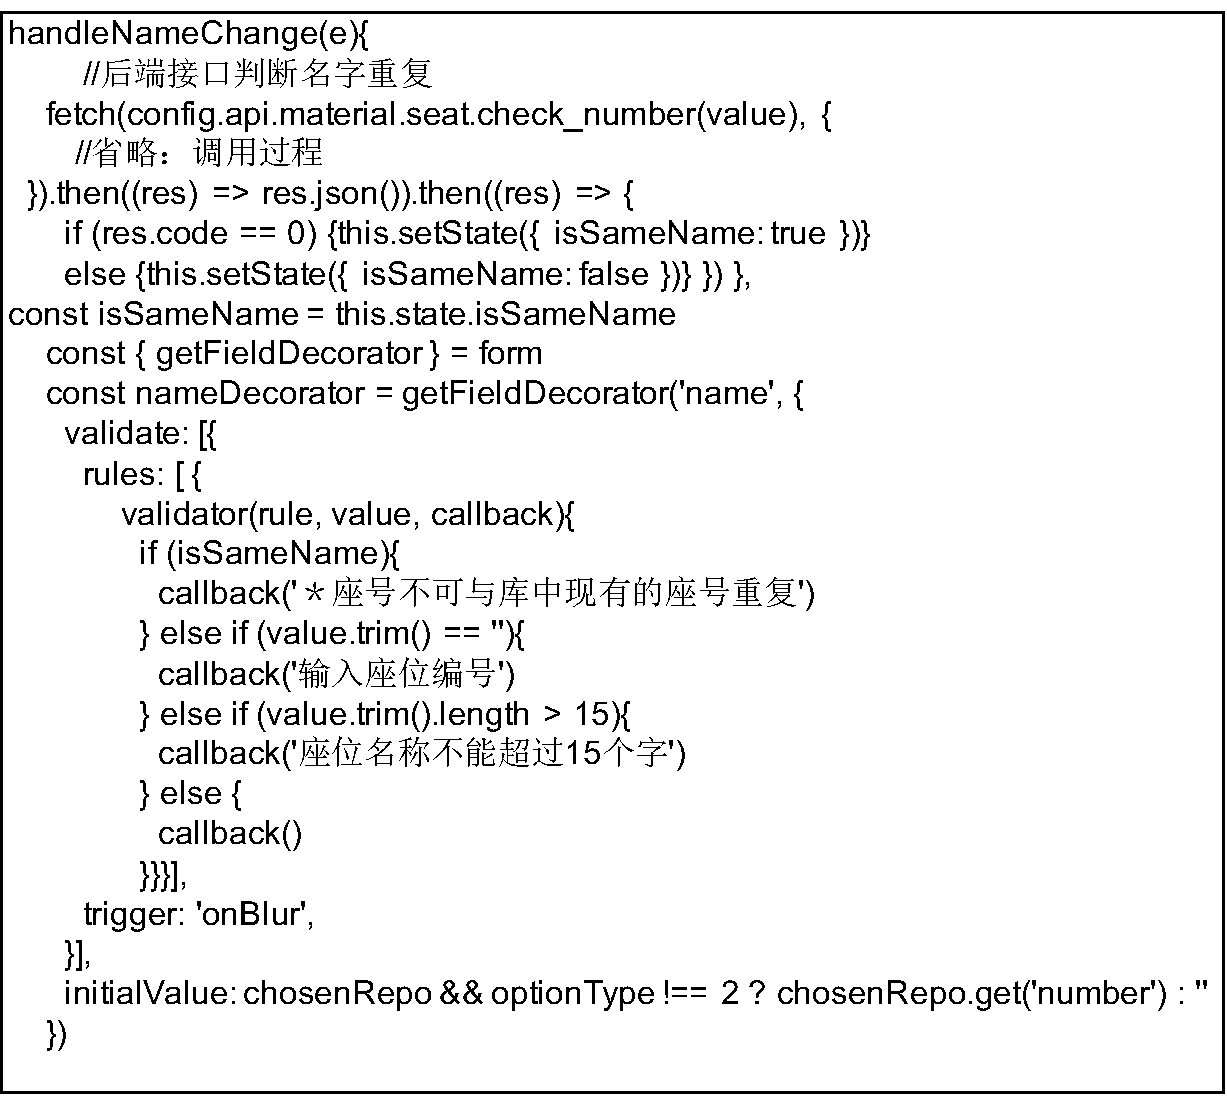
\includegraphics[width=4.5in]{FIGs/chapter4/8.pdf}
    \caption{前端AddSeatModal类渲染界面部分代码}\label{fig_seat_8}
\end{figure}

如图~\ref{fig_seat_8}代码所示是创建座位时,前端对座位名称的限制,座位号必填,不可与座位库中现有的座号重复而且字数限制在15字符以内。代码自定义编写了一个校验座位名称输入的规则,需要调用后端接口判断座位名是否与数据库存储内容重复。

\begin{figure}[htbp!]
    \centering
    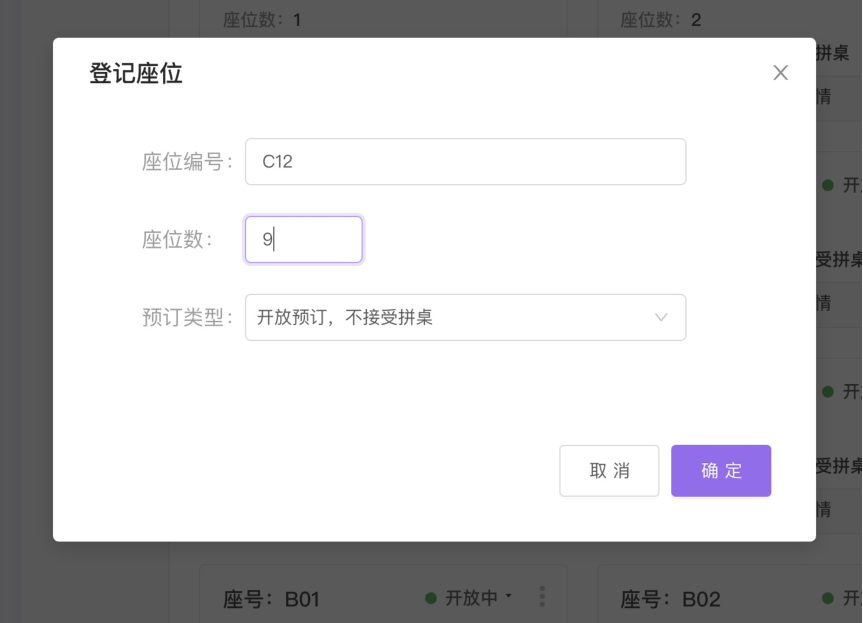
\includegraphics[width=3.8in]{FIGs/chapter4/seat_add.pdf}
    \caption{登记座位}\label{fig_seat_add}
\end{figure}

如图~\ref{fig_seat_add}所示为登记座位页面,用户需要输入座位编号、座位数以及预订类型,点击确定完成座位的登记。

座位登记完,座位库会进行刷新显示最新的座位列表,商家可以点击相应座位查看座位详情。顾客在座位可用情况下,可以用手机扫描座位二维码进入点餐页面。

\begin{figure}[htbp!]
    \centering
    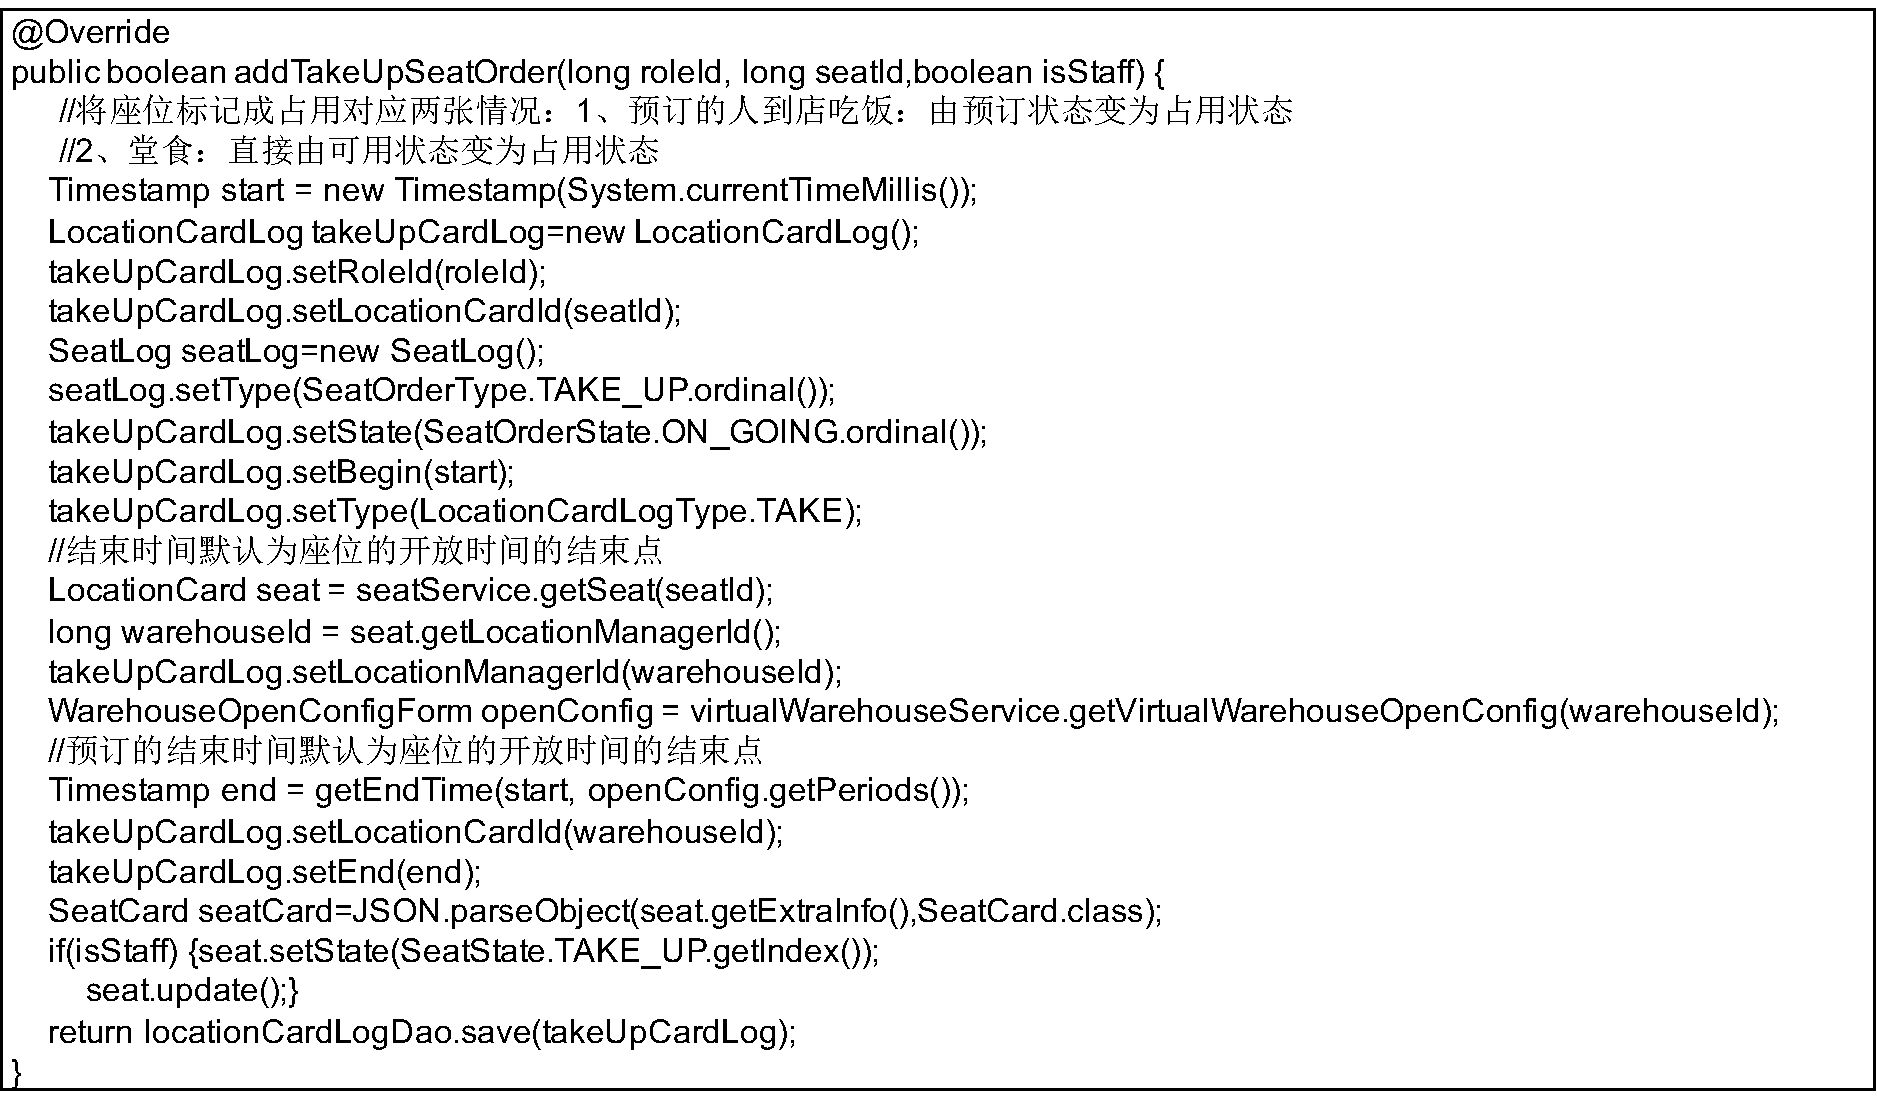
\includegraphics[width=\linewidth]{FIGs/chapter4/9.pdf}
    \caption{SeatOrderService类addTakeUpSeatOrder方法代码}\label{fig_seat_9}
\end{figure}

如图~\ref{fig_seat_9}所示是SeatOrderService类中addTakeUpSeatOrder方法的实现代码,该方法在顾客用餐时,将座位标记成占用状态并记录结束时间。座位变为占用状态有两种需要考虑的情况,一种是顾客到店用餐,座位直接变成占用状态;一种是顾客预约点单,在预约的相应时间段内座位会显示为占用状态。预约点单的结束时间可以由商家设置,如果未设置,则将默认为座位开放时间的结束点。代码通过SeatLog记录该座位的日志内容,包括占用情况、占用状态、开始结束时间等内容。

\begin{figure}[htbp!]
    \centering
    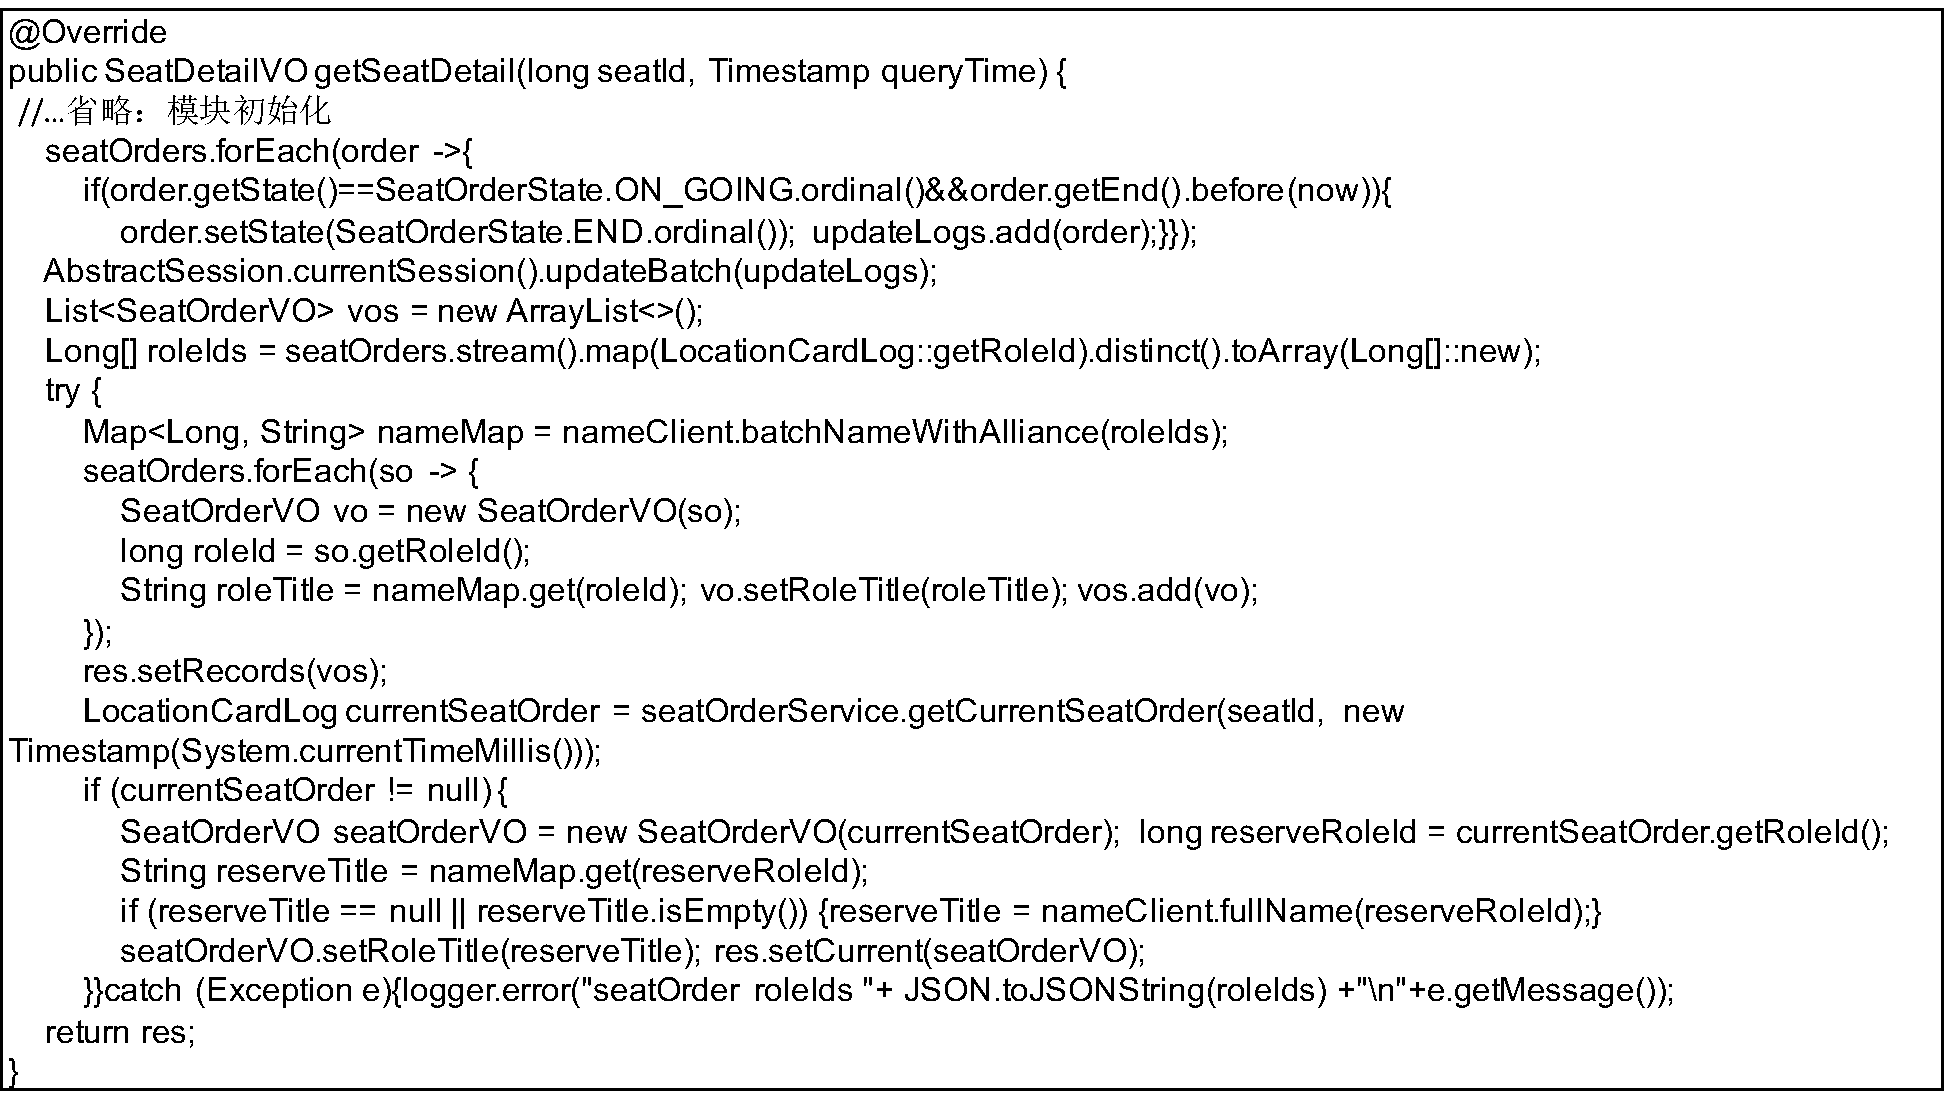
\includegraphics[width=5in]{FIGs/chapter4/10.pdf}
    \caption{SeatService类中getSeatDetail方法代码}\label{fig_seat_10}
\end{figure}

如图~\ref{fig_seat_10}所示是SeatService类中getSeatDetail方法的实现代码,该方法用于获取当天的座位详情,除了座位基本的座位号、状态、二维码、类型、当前使用情况等内容,还包括历史记录、获取座位在某时间段内的使用情况(包括预订、到店等被占用场景)。

系统获取座位详情时,需要获取座位当前的状态,根据传入的时间获取历史占用记录。座位的二维码对应相应的座号,商家可以下载二维码将其贴到餐厅的相应位置上,以供顾客扫码点单使用。当二维码有更新或者该座位停用时,商家只需要重新下载并更换二维码即可。

如图~\ref{fig_seat_detail}所示即为某一特定座位详情,可以看到完整的座位信息,点击下载座位二维码。还可以查看座位的当前操作、根据时间筛选查看不同日期的座位占用情况记录等。

\begin{figure}[htbp!]
    \centering
    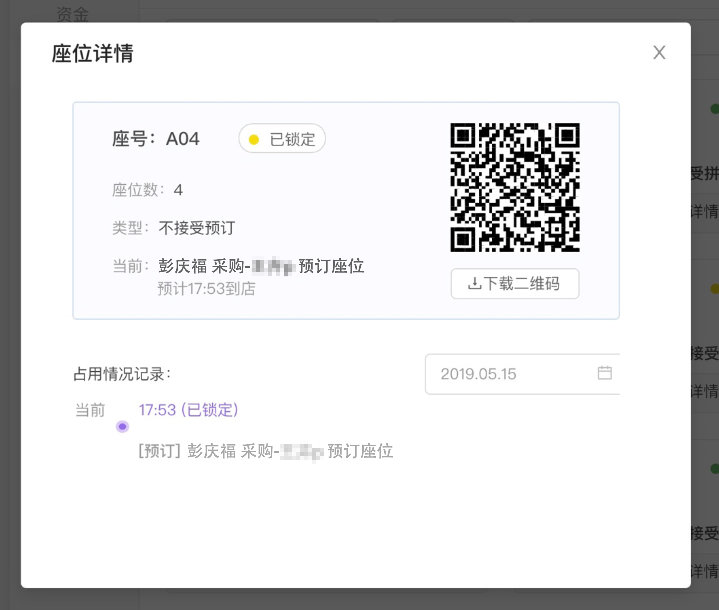
\includegraphics[width=4in]{FIGs/chapter4/seat_detail.pdf}
    \caption{座位详情}\label{fig_seat_detail}
\end{figure}

如图~\ref{fig_seat_list}所示为座位库的卡片视图,可以查看餐厅内所有座位,根据座号、状态、时间筛选座位,查看相应的座位卡片内容。有操作权限的商家可以登记座位、更改座位状态、查看座位详情,还可以选择时间轴视图、平面视图进行相应信息查看和操作。

\begin{figure}[htbp!]
    \centering
    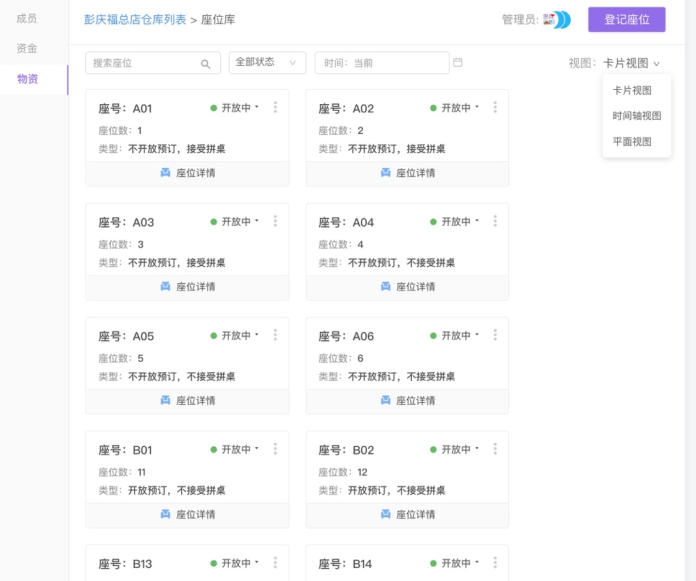
\includegraphics[width=4.5in]{FIGs/chapter4/seat_list.pdf}
    \caption{座位卡片视图列表}\label{fig_seat_list}
\end{figure}

座位库除了卡片视图,还可以切换成时间轴视图,查看特定日期内座位的使用情况。如图~\ref{fig_seat_11}所示是前端SeatTimelineContainer类中处理鼠标划到视图边缘情况的方法以及获取不开放时间段内容的代码片段,该类除了显示座位信息(包括座位号、状态、可用人数等),还显示座位在某一日期内24小时的占用情况(包括预订、占用中等),根据餐厅的开放时间以及各个座位的历史状态进行渲染。

如图~\ref{fig_seat_time_view}所示为座位库的时间轴视图界面,商家除了可以在该界面登记座位外,还可以根据不同日期来筛选查看座位使用情况的历史记录。

座位库除了以上两种视图外,还可以切换成平面视图,该视图结合了React封装的高德地图组件React-AMap,可以使用高德地图,也可以导入本地图片做地图,对地图上位置画圈或者打点来关联座位。
将相关联的座位卡片拖到地图上即可进行位置打点,也可以在地图上画一个完整的多边形区域,将卡片拖拽进区域内与位置相关联。

平面视图主要为了将餐厅与线下实际位置绑定,顾客可以在地图上直观看到区域划分。防止虚假定位欺骗消费者,也方便商家将餐厅内部的座位布局上传到系统内,与座位库的座位进行关联绑定,更方便直观的管理餐厅普通座位、拼桌座位、包厢等。

\begin{figure}[htbp!]
    \centering
    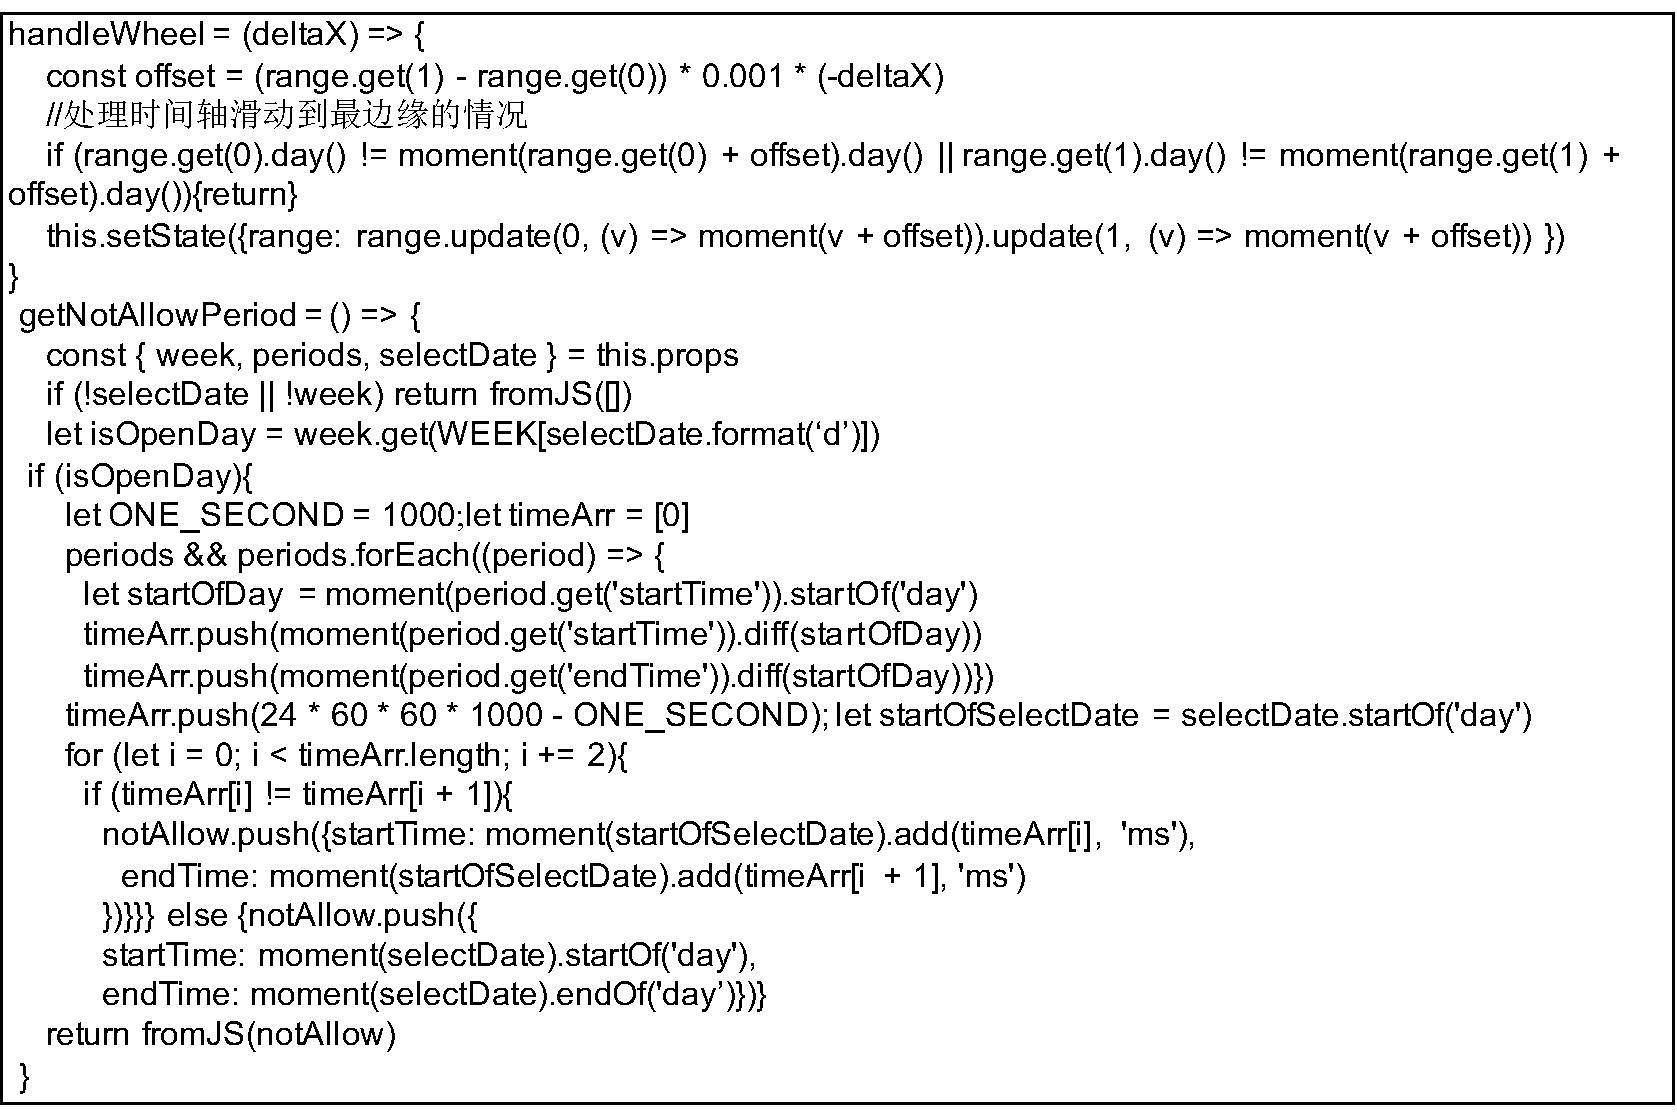
\includegraphics[width=4.5in]{FIGs/chapter4/11.pdf}
    \caption{实现时间轴视图SeatTimelineContainer类代码片段}\label{fig_seat_11}
\end{figure}

\begin{figure}[htbp!]
    \centering
    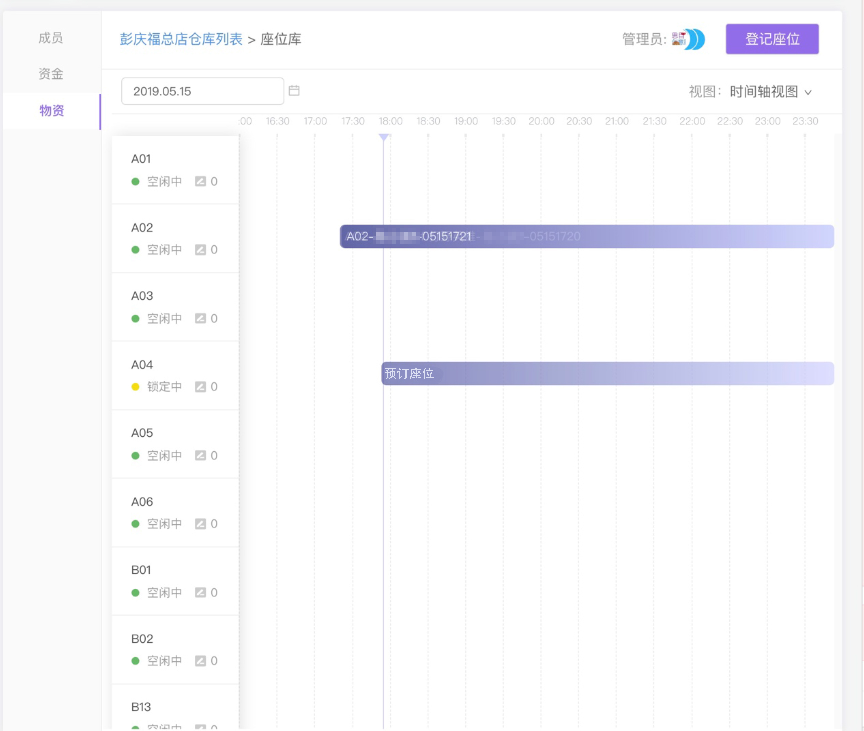
\includegraphics[width=4.2in]{FIGs/chapter4/seat_time_view.pdf}
    \caption{座位库时间轴视图}\label{fig_seat_time_view}
\end{figure}

如图~\ref{fig_seat_12}所示为前端FlatViewContainer类部分代码,引入了React封装的高德地图组件的类库React-AMap中Map、Marker组件,自定义编写了组件类MouseToolPlugin实现地图上的自定义操作,地图更换为本地导入的图片时,该类会判断并刷新界面,将之前地图上存在的点、多边形区域和相关联的座位卡片信息清除。

\begin{figure}[htbp!]
    \centering
    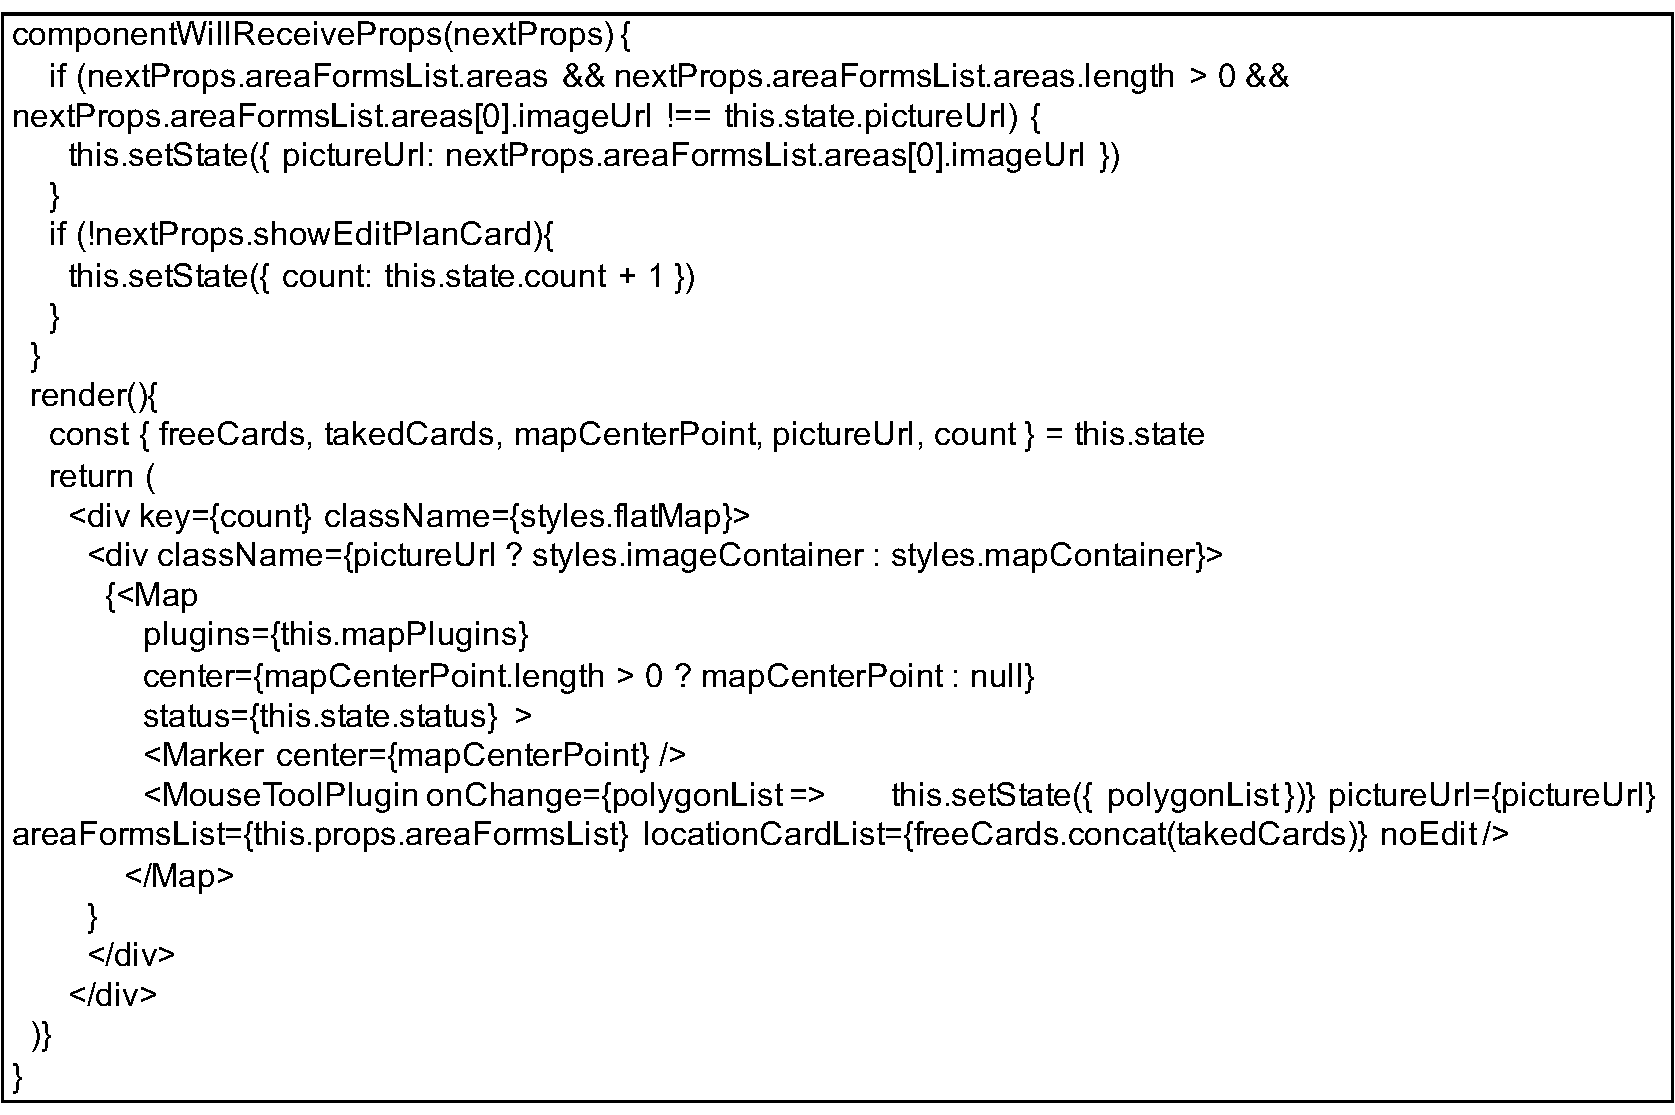
\includegraphics[width=5in]{FIGs/chapter4/12.pdf}
    \caption{实现平面视图FlatViewContainer类代码片段}\label{fig_seat_12}
\end{figure}

如图~\ref{fig_seat_13}所示,是前端类MouseToolPlugin中绘制包括地图、座位卡片、多边形以及各个坐标点的方法handleDrawAll。该方法从后端获取历史数据并渲染到地图中(包括多边形、位置点的构造),实现了将座位卡片拖到指定区域的操作,地图可以随意放大或缩小,画出的多边形区域也会随之改变。

系统需要判断平面视图的底图是高德地图还是用户自定义上传的餐厅图片,如果是地图则直接引入React-AMap组件地图,在此基础进行简单修改即可,该组件支持任意程度的放大、缩小、移动。
如果是用户上传的自定义图片,需要进行边界校验,当图片显示为100\%的时候,禁止缩小与移动,保证图片填充满整个地图界面,图片放大时才可以拖拽图片,当到达图片边缘时,图片不能再往边缘方向拖动。

\begin{figure}[htbp!]
    \centering
    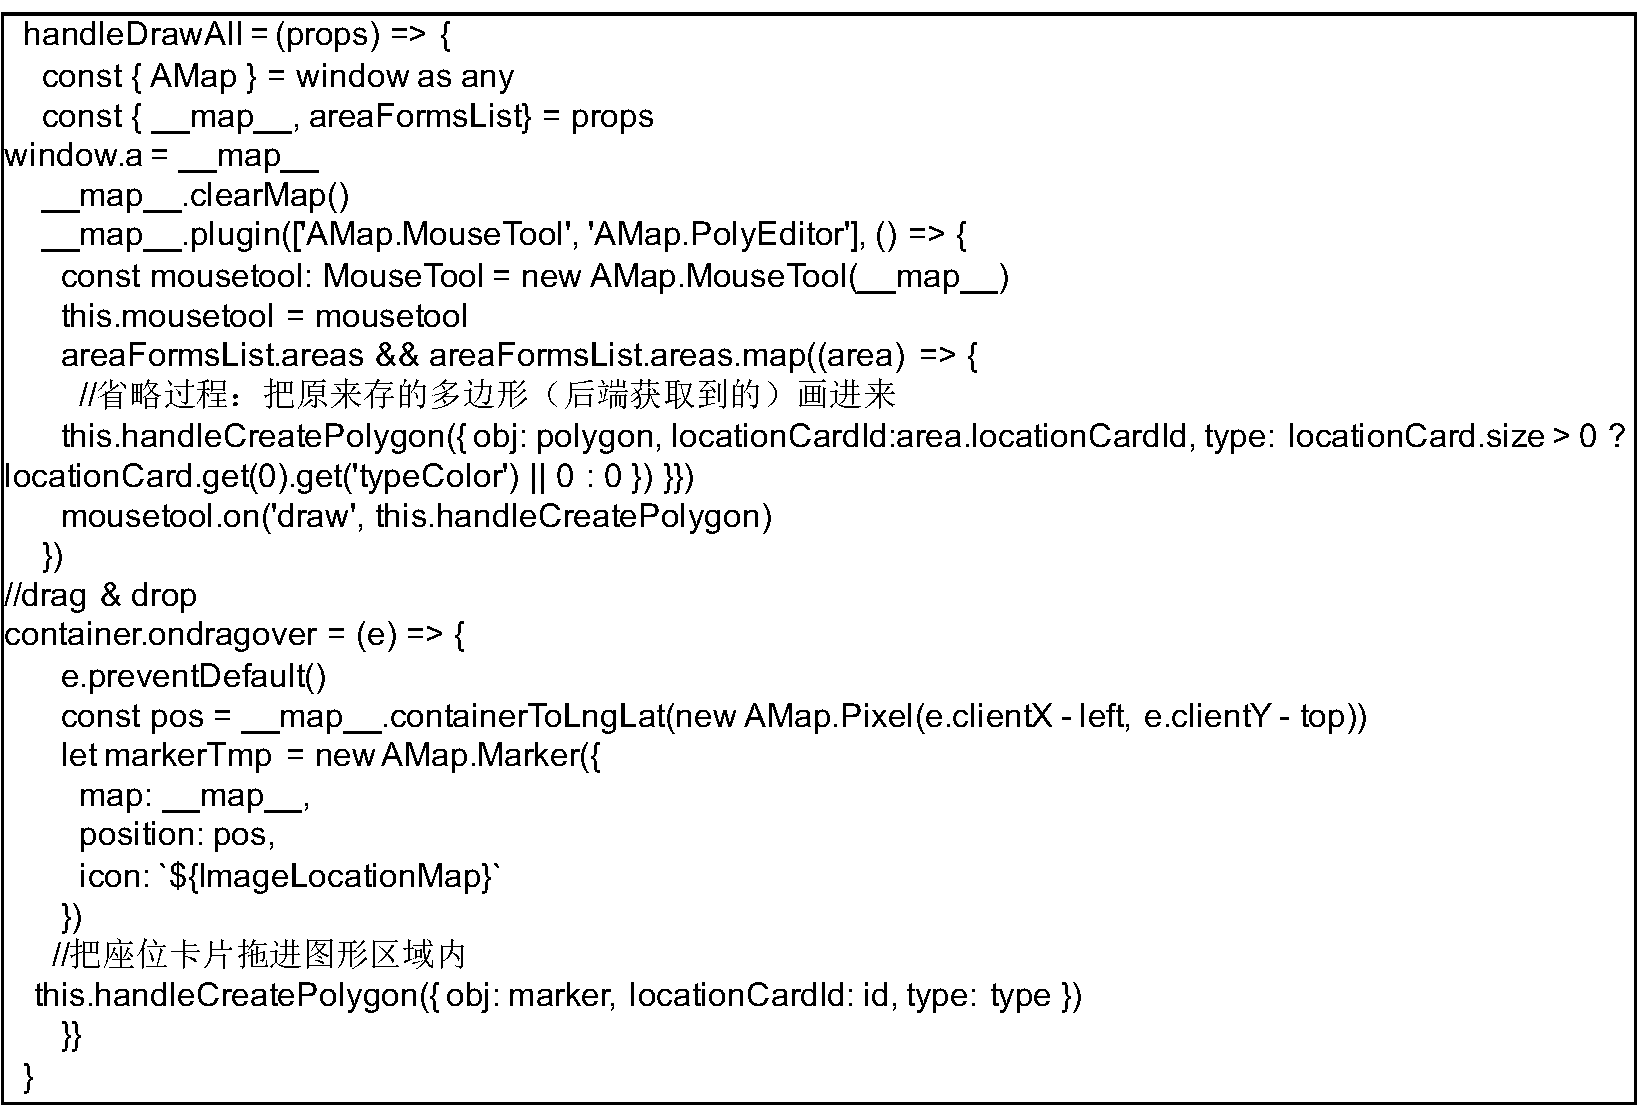
\includegraphics[width=4in]{FIGs/chapter4/13.pdf}
    \caption{MouseToolPlugin类handleDrawAll方法代码}\label{fig_seat_13}
\end{figure}

\begin{figure}[htbp!]
    \centering
    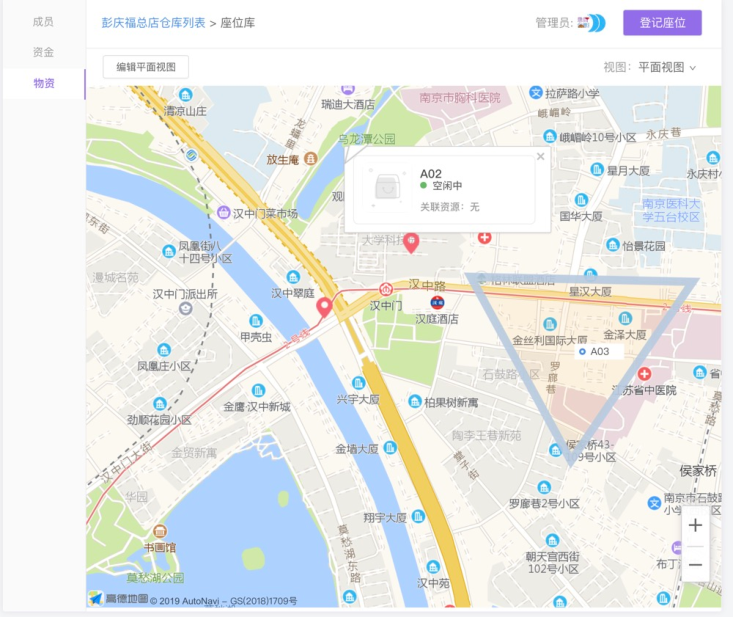
\includegraphics[width=4in]{FIGs/chapter4/seat_map.pdf}
    \caption{座位库平面视图}\label{fig_seat_map}
\end{figure}

如图~\ref{fig_seat_map}是座位库的平面视图,地图中的多边形区域和坐标点都有与之相关联的座位卡片。鼠标点击某个点或者某个多边形中的座位号时,即显示图中具体的座位信息内容,包括座号、状态、关联资源等内容。

如图~\ref{fig_seat_map_edit}所示为编辑平面视图界面,默认地图会显示当前位置,用户可以点击导入平面布局图,可以上传自定义图片。用户可以将右边的座位卡片拖拽到左边地图中形成一个坐标点,点击即可查看相关联的座位信息;也可以先在左边地图中用钢笔工具画出一个闭环的多边形区域,再将座位卡片拖拽进多边形实现位置与卡片相关联。

\begin{figure}[htbp!]
    \centering
    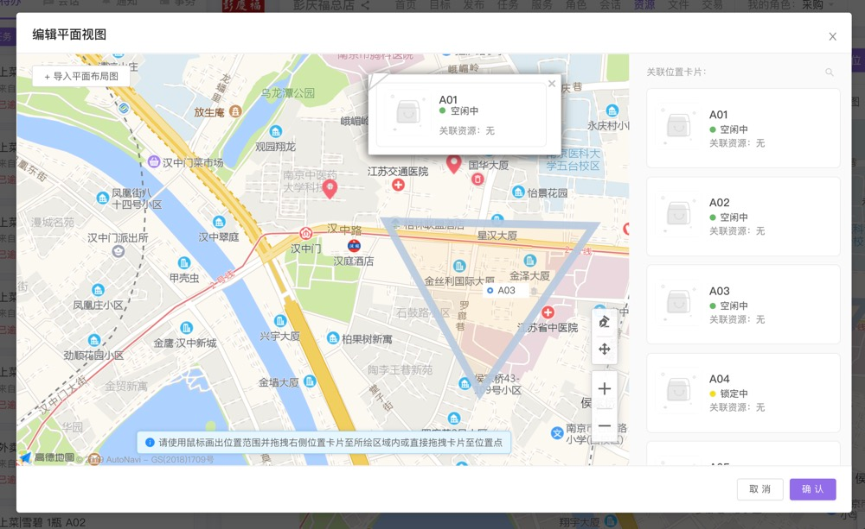
\includegraphics[width=5in]{FIGs/chapter4/seat_map_edit.pdf}
    \caption{编辑平面视图}\label{fig_seat_map_edit}
\end{figure}

\section{出品发布模块}
\subsection{出品发布模块介绍}
出品发布模块主要负责每日出品计划、菜品计划、管理餐厅营业时间等,对外提供商家营业信息、出品计划、菜品信息等接口。\\

\subsection{出品发布模块详细设计}
\begin{figure}[htbp!]
    \centering
    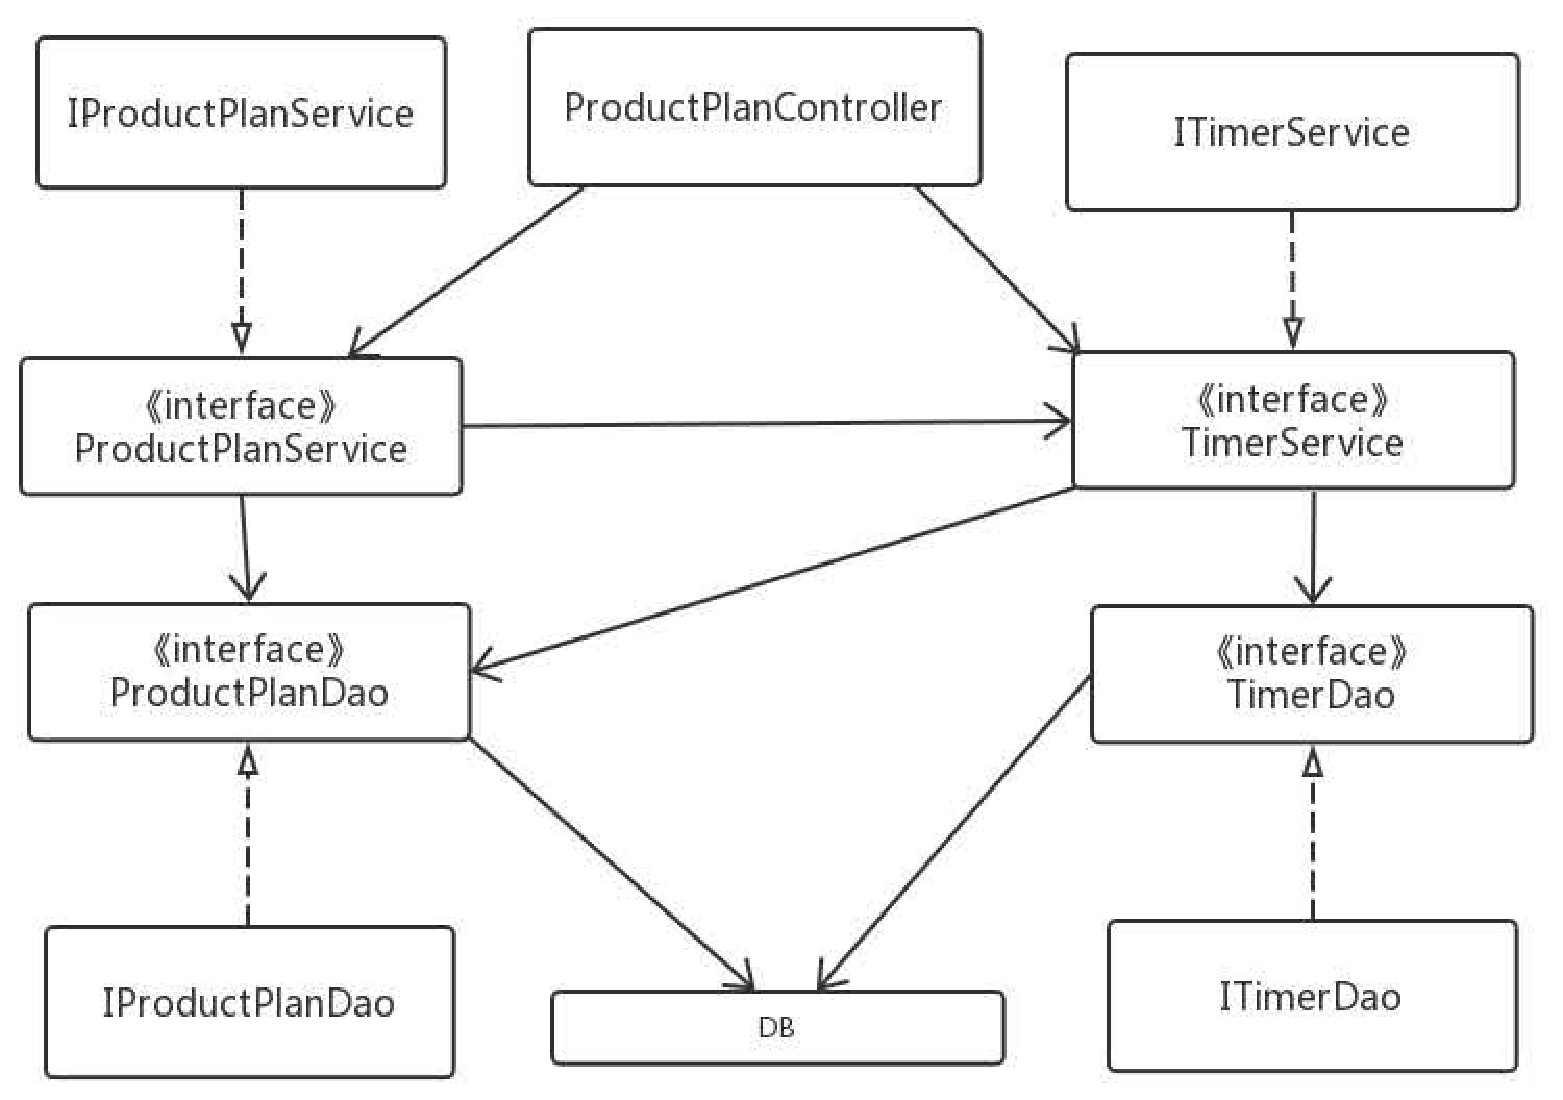
\includegraphics[width=4in]{FIGs/chapter4/dish.pdf}
    \caption{出品发布模块类图}\label{fig_dish}
\end{figure}

如图~\ref{fig_dish}所示是出品发布模块的类图,这里涉及的几个类分别是:ProductPlanController类是出品发布控制接口,可以创建、修改、删除出品发布,保存草稿,获取菜单,获取开放时间,增删改出品发布时间段等。

ProductPlanService类是出品发布服务接口,主要提供增删改查出品计划、获取出品发布详情、上架出品发布、根据出品发布获取菜单、获取当前上架的发布ID等服务,其中IProductPlanService是它的实现类。

TimerService类是出品时间段管理服务接口,主要提供增删改出品发布时间段、获取餐厅营业的所有时间段、获取当前时间段等服务,其中ITimerService是它的实现类。

ProductPlanDao主要通过出品发布ID或者菜单获得、更新、修改、批量删除出品计划列表等基本操作,其中IProductPlanDao是它的实现类。

TimerDao主要用于提供时间相关基本操作,比如通过ID获取时间段、删除时间段、获取当前开始或者结束出品计划的时间、批量获取时间段等,其中ITimerDao是它的实现类。\\

\subsection{出品发布模块实现}

\begin{figure}[htbp!]
    \centering
    \includegraphics[width=4.5in]{FIGs/chapter4/dish_time.pdf}
    \caption{创建出品发布的时序图}\label{fig_dish_time}
\end{figure}

如图~\ref{fig_dish_time}所示是ProductPlanController类create方法的执行时序图,用户点击新建出品发布,填写完相应内容后,点击创建会调用ProductPlanService类中的createProductPlan方法,进而调用ProductPlanDao的getProductPlanByAnnId将出品发布内容保存到数据库中,并返回相应的发布ID。

如果是简单的创建出品发布,系统通过发布ID获取发布详情并返回给前端。如果是复用已有的出品发布进行创建,系统会根据复用的发布ID去获取该复用发布的出品发布详情,包括餐厅当日营业时间段、菜品列表等内容,并将其更新到创建的发布内容中,使用户不必重复创建相同内容,减少工作量。后端返回该发布ID,系统根据ID获取具体的发布详情,进行界面渲染。

\begin{figure}[htbp!]
    \centering
    \includegraphics[width=5in]{FIGs/chapter4/14.pdf}
    \caption{ProductPlanService类createProductPlan方法代码}\label{fig_dish_14}
\end{figure}

如图~\ref{fig_dish_14}所示是ProductPlanService类中createProductPlan方法的实现代码,该方法用于商家创建出品发布,需要填写相应的出品计划,包括商家一天的营业时间段、是否复用之前的出品发布、选择的菜品等操作。后端会判断出品时间段是否有重复,若是则提示用户更改时间段,用户填写内容无误并成功创建出品发布后,系统返回该出品发布的发布ID。

\begin{figure}[htbp!]
    \centering
    \includegraphics[width=4in]{FIGs/chapter4/15.pdf}
    \caption{TimerService类中editTimer方法代码}\label{fig_dish_15}
\end{figure}

如图~\ref{fig_dish_15}所示是TimerService类中editTimer方法的实现代码,该方法用于修改当天出品发布的出品时间段。餐厅可能需要将营业时间分为早上营业时间、中午营业时间、晚上营业时间等多个时间段,所以修改时间段时除了需要判断结束时间不得早于开始时间,还需要判断出品时间段是否有重复,要修改的时间段是否已经有订单等。

\begin{figure}[htbp!]
    \centering
    \includegraphics[width=3.2in]{FIGs/chapter4/dish_detail.pdf}
    \caption{出品发布详情}\label{fig_dish_detail}
\end{figure}

如图~\ref{fig_dish_detail}所示为出品发布详情界面,由于该发布复用了之前的发布内容,所以创建后默认有与复用发布相同的营业时间段和出品计划菜单,商家可以修改当前发布的出品时间段、编辑时间段内的菜品种类及数量,查看采购需求、生产实况,及时上架、更新出品计划。

\section{本章小结}
本章首先讲解了彭庆福餐厅点单系统各个模块的依赖关系,接着分别描述了系统六个主要模块——订单发布模块、支付模块、用户管理模块、统计报表模块、座位管理模块和出品发布模块的详细设计与具体实现,通过模块类图、方法时序图、代码片段以及前端界面图来展示模块的实现细节与运行结果。

\chapter{系统测试}
本章基于彭庆福餐厅点单系统的设计与实现给出相应的测试介绍,主要包括测试与开发环境、部分测试的用例分析、测试的设计与实现以及测试结果。从而保障系统功能上的可用性、安全性、稳定性等,方便系统上线、使用和后期功能的扩展。
\section{系统测试环境}
\subsection{测试与开发环境}
本系统的测试环境主要有两部分,包括线下开发环境与预上线环境。线下开发环境部署在本地电脑上,环境配置如表~\ref{table:textEnvironment}所示,后端编码使用JDK1.8环境,IDEA作为集成开发工具,前端编码使用VS Code,使用Maven进行包管理,Gitlab作为代码变更管理,单元测试使用JUnit单元测试框架。

\begin{table}[htbp!]\footnotesize
    \centering
    \caption{线下开发与测试环境}
    \vspace{2mm}
    \begin{tabular}{cp{0.6\columnwidth}}
    \toprule
    \textbf{设备与软件}&\textbf{备注}\\
    \midrule 
    \textbf{系统}& MacOs Mojava 10.14.5\\
    \hline
    \textbf{磁盘}& Macintosh HD 256GB\\
    \hline
    \textbf{处理器}& 2.3GHZIntel Core i5(四核)\\
    \hline
    \textbf{语言}& JDK 1.8.0.191\\
    \hline
    \textbf{开发测试软件}& IntelliJ IDEA 2018.3、VS Code、Chorme Debug、JUnit\\
    \hline
    \textbf{项目管理软件}& Maven 3.5.0、Gitlab\\
    \bottomrule
    \end{tabular}
    \label{table:textEnvironment}
\end{table}

\begin{table}[htbp!]\footnotesize
    \centering
    \caption{预上线集成与测试环境}
    \vspace{2mm}
    \begin{tabular}{cp{0.6\columnwidth}}
    \toprule
    \textbf{设备与软件}&\textbf{备注}\\
    \midrule 
    \textbf{系统}& Linux系统\\
    \hline
    \textbf{磁盘}& 60GB\\
    \hline
    \textbf{处理器}& 四核\\
    \hline
    \textbf{内存}& 16GB\\
    \hline
    \textbf{机型}& Docker虚拟机\\
    \hline
    \textbf{软件部署}& Nginx,TomCat、Jenkins\\
    \bottomrule
    \end{tabular}
    \label{table:textEnvironment2}
\end{table}

线下环境开发完成并进行过系统单元测试之后,基本功能在本地已经验证过,之后便可以部署到预上线环境,进行相关功能模块的测试与验证。
预上线环境配置如表~\ref{table:textEnvironment2}所示,与实际生产环境基本一致,都是使用Docker对部署组件服务和业务逻辑服务进行容器化部署。通过与实际生产一致的环境部署,对系统功能做进一步的测试,尽可能找出并修改系统中潜在的bug及缺陷。\\

\subsection{测试思路}
测试是为了保证系统的各个模块功能流程正常,保证用户在使用过程的流畅性、准确性。系统一共分为两部分环境测试,一种是线下开发测试,一种是预上线集成测试。
\begin{itemize}
    \item 线下开发测试:测试各个功能模块,覆盖到系统所有模块,检验功能实现是否满足业务逻辑的要求,在设计与代码实现上是否存在缺陷或漏洞。测试会对各个功能模块的边界值、类型、返回结果等做检验,保证各接口功能的正常通信,使得系统在使用时功能逻辑正常且运行稳定。
    \item 预上线集成测试:模拟实际生产环境对系统的运行性能、压力进行测试。找出一些线下无法发现,但是影响线上用户体验感的漏洞,可以快速修复性能上的一些bug,对系统作出整体评估。
\end{itemize}

\section{系统测试过程与结果}
\subsection{功能测试}
本节将根据彭庆福点单系统主要的功能性需求部分进行用例测试的描述。

1.到店多次下单功能测试
\begin{table}[htbp!]
    \footnotesize
    \centering
    \caption{到店多次下单功能测试用例}
    \vspace{2mm}
    \begin{tabular}{cp{11.5cm}}
     \hline
     \ 测试用例编号 & TN1 \\ 
     \hline
     \ 测试内容 & 顾客针对同一座位多次下单 \\ 
     \hline
     \ 测试功能 & 系统能够识别用户的多次扫码,保证一个座位同一时刻只能存在单个订单 \\ 
     \hline
     \multirow{4}{*}{测试步骤}
      & 1.	顾客扫桌上二维码,选择菜品下单\\
      & 2.	系统下单成功后,显示订单详情\\
      & 3.	顾客再次扫描该座位二维码\\
      & 4.	系统显示顾客已有订单的详情\\
      & 5.	更换不同顾客扫描该座位二维码\\
      & 6.	系统提示该座位已有订单,无法下单\\
     \hline
     \multirow{1}{*}{预期结果}
      & 1. 顾客连续扫码时,系统能够识别并显示该顾客未完成的订单内容,顾客可以对该订单加菜、结账等\\
      & 2. 当其他顾客在该座位扫码时,系统能够识别出该座位号有未结账的订单,提示顾客更换座位点单\\
    \hline
    \end{tabular}
    \label{table:tn1}
\end{table}

如表~\ref{table:tn1}所示,这一部分的功能测试主要针对顾客多次扫码下单以及不同顾客对同一座位扫码下单的情况,看系统能否有效进行拦截,并给出不同的提示信息。

2.偏远地区外卖点单功能测试

如表~\ref{table:tn2}所示,这一部分的功能测试主要针对订单发布模块,看系统能否有效拦截恶意外卖点单。
\begin{table}[htbp!]
    \footnotesize
    \centering
    \caption{偏远地区外卖点单功能测试用例}
    \vspace{2mm}
    \begin{tabular}{cp{11.5cm}}
     \hline
     \ 测试用例编号 & TN2 \\ 
     \hline
     \ 测试内容 & 顾客选择的配送地点超过商家配送范围 \\ 
     \hline
     \ 测试功能 & 系统能阻止顾客下单超过配送范围的订单,外卖订单一旦被商家接单且未超过配送时间,无法取消 \\ 
     \hline
     \multirow{2}{*}{测试步骤}
      & 1.	顾客选择外卖点单,配送地址填写一个偏远地址,填写其余内容并选菜下单\\
      & 2.	系统获取配送地址,提醒用户该餐厅配送范围超出,无法下单 \\
      & 3.	商家接单后,订单界面的取消订单按钮消失 \\
     \hline
     \multirow{1}{*}{预期结果}
      & 1. 系统能够识别出超出配送范围的外卖订单,并进行有效拦截\\
      & 2. 系统能够识别出订单被商家接单且未超过配送时间,并隐藏取消订单按钮\\
    \hline
    \end{tabular}
    \label{table:tn2}
\end{table}

3.顾客微信、支付宝支付功能测试

如表~\ref{table:tn3}所示,这一部分的功能测试主要针对支付模块,顾客可以通过微信、支付宝、浏览器等多种方式进行扫码点餐,不同的客户端环境中系统提供给用户的付款方式不同,因此需要测试显示给用户的支付方式是否与用户实际选择的一致。
\begin{table}[htbp!]
    \footnotesize
    \centering
    \caption{支付功能测试用例}
    \vspace{2mm}
    \begin{tabular}{cp{11.5cm}}
     \hline
     \ 测试用例编号 & TN3 \\ 
     \hline
     \ 测试内容 & 测试顾客支付功能 \\ 
     \hline
     \ 测试功能 & 顾客选择支付方式与系统实际展示的支付方式是否一致 \\ 
     \hline
     \multirow{2}{*}{测试步骤}
      & 1.	顾客通过支付宝扫码下单,进行支付结账\\
      & 2.	系统展示支付宝付款页面 \\
      & 3.	顾客通过微信扫码下单,进行支付结账\\
      & 4.	系统展示微信付款页面 \\
      & 5.	顾客通过浏览器扫码下单,进行支付结账\\
      & 6.	系统提示用户选择支付方式(微信或者支付宝),根据用户选择情况跳转到相应付款页面 \\
     \hline
     \multirow{1}{*}{预期结果}
      & 1. 当扫码源为微信界面时,系统只提供微信支付方式\\
      & 2. 当扫码源为支付宝界面时,系统只提供支付宝支付方式\\
      & 3. 当扫码源为浏览器时,系统提供微信、支付宝支付方式供用户选择,并根据其选择进行相应付款界面跳转\\
    \hline
    \end{tabular}   
    \label{table:tn3}
\end{table}

4.用户角色功能测试

如表~\ref{table:tn4}所示,这一部分的功能测试主要针对用户管理模块。点餐系统中顾客一共包含两种角色:企业员工角色以及普通顾客角色。餐厅会与某些企业开展合作,如果企业员工到店就餐,可以给予不同程度的折扣优惠。因此需要测试用户切换角色进行下单时,系统是否能够准确判定。
\begin{table}[htbp!]
    \footnotesize
    \centering
    \caption{用户角色功能测试用例}
    \vspace{2mm}
    \begin{tabular}{cp{11.5cm}}
     \hline
     \ 测试用例编号 & TN4 \\ 
     \hline
     \ 测试内容 & 顾客选择不同的角色进行下单 \\ 
     \hline
     \ 测试功能 & 系统能根据不同的用户角色给出不同的订单优惠 \\ 
     \hline
     \multirow{4}{*}{测试步骤}
      & 1.顾客选择某公司员工角色,并点菜下单\\
      & 2.系统识别用户角色,在计算用户支付金额时根据该公司的优惠政策进行打折 \\
      & 3.顾客选择普通顾客角色,并点菜下单 \\
      & 4.系统识别用户角色,在计算用户支付金额时不打折\\
      \hline
     \multirow{1}{*}{预期结果}
      & 1. 系统能够准确识别用户角色,并能够准确匹配该角色对应的折扣优惠政策\\
    \hline
    \end{tabular}   
    \label{table:tn4}
\end{table}

5.统计报表功能测试

如表~\ref{table:tn5}所示,这一部分的功能测试主要针对统计报表模块。商家通过统计报表的功能可以查看本餐厅所有菜品的进销存情况,并根据此报表制定采购计划。商家还可以通过统计报表根据日、周、月、年等维度查看营收情况,并根据报表计算餐厅利润情况。需要测试菜品进销存报表、餐厅营收报表是否和数据库中对应的订单流水数据一致,保证商家查看到准确数据。

\begin{table}[htbp!]
    \footnotesize
    \centering
    \caption{统计报表功能测试用例}
    \vspace{2mm}
    \begin{tabular}{cp{11.5cm}}
     \hline
     \ 测试用例编号 & TN5 \\ 
     \hline
     \ 测试内容 & 测试商家的菜品进销存报表以及餐厅营收报表 \\ 
     \hline
     \ 测试功能 & 报表数据应与数据库数据一致 \\ 
     \hline
     \multirow{4}{*}{测试步骤}
      & 1. 商家查看当日菜品进销存报表\\
      & 2. 系统显示报表信息 \\
      & 3. 商家查看当日营收报表 \\
      & 4. 系统显示报表信息\\
      \hline
     \multirow{2}{*}{预期结果}
      & 1. 系统展示的菜品进销存报表信息与当日所有订单流水对应\\
      & 2. 系统展示的营收报表信息与当日所有订单流水对应\\
    \hline
    \end{tabular}   
    \label{table:tn5}
\end{table}

6.出品发布功能测试

如表~\ref{table:tn6}所示,这一部分的功能测试主要针对出品发布模块,商家可以通过每日出品发布查看各菜品的库存情况,防止出现菜品售罄,而用户可以继续下单的情况。这种情况会给顾客带来不好的用户体验,影响餐厅形象。需要保证顾客在非餐厅营业时间内点餐时,系统提示用户当前时间无法用餐,可以预约点单,防止出现用户下单,而餐厅未营业的情况。因此需要测试餐厅发布的出品计划与顾客查看到的餐厅信息是否一致。
\begin{table}[htbp!]
    \footnotesize
    \centering
    \caption{出品发布功能测试用例}
    \vspace{2mm}
    \begin{tabular}{cp{11.5cm}}
     \hline
     \ 测试用例编号 & TN6 \\ 
     \hline
     \ 测试内容 & 测试商家的出品计划发布功能\\ 
     \hline
     \ 测试功能 & 商家发布的出品计划应与顾客在点单消费过程中查看到的信息一致 \\ 
     \hline
     \multirow{4}{*}{测试步骤}
      & 1. 商家将某一菜品的库存设置为0\\
      & 2. 系统在顾客点单时显示菜品为已售罄\\
      & 3. 商家设置营业时间\\
      & 4. 顾客不在餐厅的营业时间段内点单时,系统需要提醒用户当前时间无法用餐,可以预约点单\\
      \hline
     \multirow{2}{*}{预期结果}
      & 1. 系统展示给顾客的营业时间与商家发布的一致\\
      & 2. 系统展示的菜品库存与商家设置的一致\\
    \hline
    \end{tabular}   
    \label{table:tn6}
\end{table}

7.座位管理功能测试

如表~\ref{table:tn7}所示,这一部分的功能测试主要针对座位管理模块,商家需要将座位信息,包括座位号、对应二维码等信息录入系统,在餐厅座位上张贴对应的二维码,方便顾客点餐。并且商家可以实时查看餐厅座位的占用情况,调整餐厅座位排布,为顾客提供更好的用餐体验。
因此需要测试餐厅的实际占用情况是否和商家查看的座位视图一致。由于座位信息会对应到顾客的订单信息时,还需要测试商家发布的座位信息是否与订单流水中的一致,防止出现二维码与座位不对应的情况。\\

\begin{table}[htbp!]
    \footnotesize
    \centering
    \caption{座位管理功能测试用例}
    \vspace{2mm}
    \begin{tabular}{cp{11.5cm}}
     \hline
     \ 测试用例编号 & TN7 \\ 
     \hline
     \ 测试内容 & 测试餐厅座位管理功能\\ 
     \hline
     \ 测试功能 & 餐厅的实际座位情况与商家查看的座位视图一致 \\ 
     \hline
     \multirow{6}{*}{测试步骤}
      & 1. 商家登记餐厅座位信息,包括座号、二维码、座位数、占用情况等信息\\
      & 2. 系统保存商家修改\\
      & 3. 顾客扫描某一座位上的二维码进行点餐并下单\\
      & 4. 系统下单成功,显示订单信息、座位信息\\
      & 5. 商家查看当前餐厅的座位列表\\
      & 6. 系统显示实时座位列表,展示被占用的座位和空闲座位\\
      \hline
     \multirow{1}{*}{预期结果}
      & 1. 系统展示给商家的座位列表内容与顾客下单情况一致\\
    \hline
    \end{tabular}   
    \label{table:tn7}
\end{table}

\subsection{性能测试}
为了保障顾客在高峰用餐时段的良好用户体验,需要对餐厅点单系统进行性能测试。性能测试分为两个部分,分别是到店点餐性能测试以及外卖点餐性能测试。

由于餐厅座位有限,在进行到店点餐性能测试时,可以参考餐厅最大座位数。目前餐厅座位数为100,对餐厅点单系统模拟每分钟有100个用户请求点餐下单。在进行外卖点餐性能测试时,对餐厅点单系统模拟每分钟有200个用户请求点餐下单。分别测试系统的平均响应时间和内存占用率,衡量系统性能。

在测试过程中,通过Linux的常用监控命令查看CPU占用率,并通过测试工具平台查看接口的平均响应时间。到店点餐的平均响应时间为300ms,CPU占用率小于30\%,外卖点餐的平均响应时间为250ms,CPU占用率小于40\%。测试结果表明系统的性能良好,能够保证在高峰就餐段系统的平稳运行。

\section{本章小结}
本章主要基于第三章中的需求分析对彭庆福餐厅点单系统的测试情况进行介绍。餐厅点单系统分别进行了功能测试和性能测试,测试结果表明该系统已达到需求分析部分提出的目标,并且系统的性能能够满足用户使用要求。

\chapter{总结与展望}
\section{论文工作总结}
随着互联网的发展以及餐饮行业消费者需求多样性的提高,基于互联网的餐厅点单系统应运而生,很多点单系统只简单实现了点餐功能,无法满足顾客对隐私性、安全性、个性化的要求,彭庆福餐厅点单系统从顾客和商家两个用户角度做出了不同的设计与实现,使用二次认证方式保证顾客隐私安全,推出到店点餐、预约点餐、外卖点餐三种类型供顾客下单,极大程度上带给用户方便快捷的点单体验,并为商家提供了座位管理、统计报表等功能,帮助商家降低管理餐厅的成本和精力,保存海量数据记录。

本文结合了国内外餐厅点单系统的发展状况与研究现状,介绍了彭庆福餐厅点单系统的设计,并使用了以下技术进行实现:
\begin{itemize}
    \item 后端主要使用Spring Boot和Spring Cloud,程序结构为典型的MVC结构。
    \item 使用React与Redux、Immutable.js、antd、React-AMap实现了前端界面的编写。
    \item 使用了Redis记录用户下载缓存、Session缓存。
    \item 使用Druid数据库连接池进行数据关系存储。
    \item 使用Maven工具进行项目管理、编译打包,使用了Gitlab进行项目版本管理及代码存储,从持续集成系统CI获取构建部署包。
\end{itemize}

本文对该系统进行了用例分析和架构设计,阐述了彭庆福餐厅点单系统的六个模块:订单发布模块、支付模块、用户管理模块、统计报表模块、座位管理模块和出品发布模块。在此基础上,借助详细设计类图、时序图、代码介绍和运行截图,对各模块进行了详细设计和实现的具体描述,介绍了系统的线上线下测试环境和功能测试,从而保障系统功能上的安全性和稳定性。

彭庆福餐厅点单系统自从上线使用以来,一直在平稳运行中,用户量逐步增长,并且有多家餐厅并行使用,包括一些连锁店、分店和个体店。截至2020年3月,合作的餐厅已经达到16家,注册用户超过18万人,餐厅实现了存储海量菜品、座位、订单、报表等信息。该系统基本满足了顾客与商家对于该类软件的需求。\\

\section{展望}
目前,本文介绍的彭庆福餐厅点单系统已经可以让顾客进行完整的下单操作,让商家对餐厅进行有效的管理,但系统在功能设计与会员制度上还有着比较大的进步空间。从顾客的角度来说,系统还可以增加菜品收藏、拼单推荐、在线排队、优惠券赠送、虚拟货币充值等功能;从商家角度来说,系统还可以增加会员充值赠送、会员积分、订单集体派送等功能,进一步完善系统的实用性、易用性以及个性化定制。

在后期的需求调研中我们发现顾客对系统的满意度还有待提升,主要因为没有得到很好的使用指南。不少顾客到店后依然选择叫服务员点单,没有发现餐桌上可以自主扫码点单的标示,后期会提升座位二维码以及使用教程的醒目度。商家会通过线下推广宣传以及线上优惠券、团购等服务来吸引更多的顾客关注餐厅,使用该系统。

% \chapter{表格}

表格是LaTeX中少数没有Word好用的功能。
但word的表格依然存在行间距的问题,而LaTeX也有简洁美观,相对易用(相对)的三线表。

\section{表格与表格引用的基本概念}
表格的编号和表目录都是自动生成并持续编号的,无需人工修改。
只要对表格有标注(label),则在正文中引用该表的label,就可以随时保持最新编号。

\textbf{注意:如果一个新表格加入,并被引用,编辑器将需要连续编译两次到三次,才能完成全部标题、引用和目录的更新。
可以理解为第一次编译引入新表格,此时还不知表格引用位置的具体编号,需要留待第二次编译完成。
而有可能第三次编译才将表格信息写入开头的表目录。
类似的情况也会出现在图形和论文引用这两部分,其中尤以论文引用部分最为奇特,详见相关章节。}

\section{基本表格}

表~\ref{table:codeOverlap}(这里是一个表引用!)是一个简单的三线表,双击表格可以在编辑界面内见到具体设置。

具体解释一下表格的设置:
第一个table体内首先先声明标记位置以及字体大小;
随后声明表格对齐方式;
其次描述表标题;
之后进入具体的表内容(tabular,此时还要声明表格单元中的内容如何对齐);
依次画出三线并填充内容;
如果表格内容较多,可以相应的加入横线来划分(hline);
之后退出tabular;
最后给表起名以实现全局引用,并退出表格。

\begin{table}[htb]\footnotesize
\centering
\caption{实验系统中函数调用与数据依赖的交集}
\vspace{2mm}
% l - left, r - right, c - center. | means one vertical line 这里声明的是表格单元中的内容如何对齐
\begin{tabular}{lccc}
\toprule
&\textbf{Call}&\textbf{Data}&\textbf{Overlap}\\
\midrule
\textbf{VoD}&222&899&66\\
\textbf{GanttProject}&5560&24243&1042\\
\hline
\textbf{jHotDraw}&3943&14555&893\\
\bottomrule
\end{tabular}
\label{table:codeOverlap}
\end{table}

\section{表格单元跨列}

表~\ref{table:codeSmellMethods}展示如何实现表格单元跨列。

\begin{table}[htb]\footnotesize
\centering
\caption{错误率与函数特征之间的关联}
\vspace{2mm}
% l - left, r - right, c - center. | means one vertical line
\begin{tabular}{lcccccc}
\toprule
&\multicolumn{2}{c}{\textbf{Parameters}}
&\multicolumn{2}{c}{\textbf{Return Value}}
&\multicolumn{2}{c}{\textbf{Is Constructor}}\\
&with&without&with&without&with&without\\
\midrule
\textbf{VoD}&8.99\%&9.20\%&6.10\%&9.51\%&9.43\%&8.46\%\\
\textbf{GanttProject}&9.53\%&6.05\%&8.43\%&6.71\%&5.14\%&8.09\%\\
\textbf{jHotDraw}&4.40\%&3.89\%&4.36\%&3.88\%&2.91\%&4.39\%\\
\bottomrule
\end{tabular}
\label{table:codeSmellMethods}
\end{table}

\section{表格单元跨行}

表~\ref{table:systemsCH4}展示如何实现表格单元跨行(Average Number那一行)。
此外,本表格的字体尺寸为scriptsize,比上一个表格的footnotesize要更小。

\begin{table}[htb]\scriptsize
\centering
\caption{五个实验系统概述}
\vspace{2mm}
% l - left, r - right, c - center. | means one vertical line
\begin{tabular}{lccccc}
\toprule
&\textbf{VoD}&\textbf{Chess}&\textbf{GanttProject}&\textbf{jHotDraw}&\textbf{iTrust}\\
\midrule
\textbf{Version}&-&0.1.0&2.0.9&7.2&13.0\\ \hline
\textbf{Programming Language}&Java&Java&Java&Java&Java\\ \hline
\textbf{KLOC}&3.6&7.2&45&72&43\\ \hline
\textbf{Executed methods}&165&316&2741&1755&250\\ \hline
\textbf{Evaluated requirements}&12&7&17&21&34\\ \hline
\multirow{2}{3.5cm}{\textbf{Average Number of Methods Implementing a Requirement}}&45&173&387&121&12\\
&(9-148)&(23-288)&(78-815)&(1-555)&(1-33)\\ \hline
\textbf{Size of the golden RTM}&1980&2212&46597&36855&8500\\ \hline
\textbf{Requirement traces}&534&1210&6584&2547&353\\ \hline
\textbf{Random Chance of guessing}&0.5-7.5\%&1-13\%&0.2-1.7\%&0.003-1.5\%&0.01-0.4\%\\ \hline
\textbf{Method Call Dependencies}&210&439&4830&3848&319\\ \hline
\textbf{Method Data Dependencies}&905&976&30452&17316&5329\\
\bottomrule
\end{tabular}
\label{table:systemsCH4}
\end{table}

\section{表格与图形位置}

常用选项[htbp]是浮动格式:

『h』当前位置。将图形放置在正文文本中给出该图形环境的地方。如果本页所剩的页面不够,这一参数将不起作用。

『t』顶部。将图形放置在页面的顶部。

『b』底部。将图形放置在页面的底部。

『p』浮动页。将图形放置在一只允许有浮动对象的页面上。

 一般使用[htb]这样的组合,只用[h]是没有用的。这样组合的意思就是LaTeX会尽量满足排在前面的浮动格式,就是h-t-b这个顺序,让排版的效果尽量好。图形章节会有更多位置符号的例子。


% \chapter{图形}

\section{基本图形}
相对于表格而言,LaTeX中的图形就简单多了,需要注意的是本模板推荐将所有图形都转化为pdf,具体内容参见图~\ref{fig_errorExpCH4}。
该图形放在本模板的本地文件夹FIGs中。
图~\ref{fig_errorExpCH4}是将Excel的五个子图形排布在一个ppt页面上,之后保存为pdf文件,最终得到的图形可以保证是矢量图。


\begin{figure}[htb]
  \centering
  \includegraphics[width=5in]{FIGs/chapter4/errorExpCH4.pdf}
  \caption{以含错误的RTM为输入的五个系统上三个实验(Call,Data,Call+Data)的错误率(Incorrectness)}\label{fig_errorExpCH4}
\end{figure}

\textbf{注意:不要删除FIGs下面的njulogo和njuname这两个文件,这是论文封面的校徽和手写体南大校名。}

\section{引用代码}

\begin{figure}[htb]
  \centering
  \includegraphics[width=\linewidth]{FIGs/chapter4/VoDCodeSample.pdf}
  \caption{VoD系统中的代码片段}\label{fig_VoDCodeSample}
\end{figure}

这里给出一个代码引用的推荐实践。
引用代码时先将代码放入word的文本框中,调整结束后,将该文本框页面另存为pdf文件,之后再作为图形来引用,如图~\ref{fig_VoDCodeSample}所示。




% \chapter{公式}

这里直接给出几个较为复杂的公式的例子,可一一进行参照。
若有未包含的数学符号或公式格式,请参阅本模板所包含的手册(本地manual文件夹)或百度必应谷歌。

\section{公式5.1与论证}
“从直接代码依赖的角度出发,从一个初始域外的类$C_{out}$ 出发我们尝试找到一个通往初始域内的类$C_{in}$ 的路径。一条合法的路径需要满足以下两点要求:(1)这一路径是单向的,即$C_{out}$ 传递性地到达$C_{in}$ 或$C_{in}$ 传递性地到达$C_{out}$;(2)路径中只能包含一个$C_{in}$ (为了避免重复路径的出现)。为了恰当的估计一条合法路径所代表的交互程度,我们计算路径上所有直接代码依赖的紧密度值的几何平均。我们用如下公式来重新计算给定$C_{out}$ 的IR 值($IR_{DC}$):”

\begin{align}
IR_{DC}=IR_{origin}+(IR_{top}-IR_{origin})^{\left| PATH\right|}\sqrt {\prod _{x \in PATH}Closeness_{DC}(x)} \end{align}

“其中$IR_{origin}$ 代表$C_{out}$ 的初始IR值,$IR_{top}$ 代表$C_{in}$ 被提升过的IR值,\emph{PATH} 代表$C_{out}$ 与$C_{in}$ 之间的路径内所有的直接代码依赖,而$Closeness_{DC}(x)$ 则代表每一条直接代码依赖关系的紧密度值。在同一对$C_{out}$ 和$C_{in}$ 之间可能存在多条合法路径,我们只保留其中能使$IR_{DC}$ 值最大的那条路径。”

\section{公式5.2与论证}

“由于IR 方法返回的是一个按照IR 值大小倒序排列的候选线索列表,因此一种常用的比较IR 方法的方式是在不同的查全率水平上比较不同方法之间的精确度,通常用$Precision-Recall$ 曲线表示。为了进一步衡量IR 方法返回结果的整体质量,我们选用了另外两个常用的实验度量:$AP$(Average Precision)与$MAP$ (Mean Average Precision)。其中,$AP$ 用于度量全部查询(需求)所检索的相关文档的排序质量,计算方式如下:”
\begin{align}
AP=\dfrac {\sum _{r=1}^{N}\left( Precision\left( r\right) \times isRelevant\left( r\right) \right) } {\left| RelevantDocuments\right| }
\end{align}

“其中,$r$ 表示被查询对象(类)在列表中的排序,$Precision(r)$ 表示前$r$ 个类的准确率。$isRelevant()$ 为一个二值函数,如果文档是相关的,则返回1,若无关,则返回0。”

\section{公式5.3与论证}

“由此,我们为类数据依赖定义紧密度$Closeness_{CD}$ 如下:”

\begin{align}Closeness_{CD}=\frac {\sum _{x \in \{DT_{i}\cap DT_{j}\}}idtf(x)} {\sum _{y \in \{DT_{i}\cup DT_{j}\}}idtf(y)}\end{align}

“其中$idtf(x)$ 代表共享数据类型的idtf值,$DT_i$ 与$DT_j$ 的交集代表该数据依赖上的共享数据类型,而$DT_i$ 与$DT_j$ 的并集则代表$C_i$ 和$C_j$ 在全部代码上所访问的数据类型。$Closeness_{CD}$ 的取值范围是0到1之间。”


% \chapter{算法}

同样是定义+引用的方式,参见算法~\ref{alg:Re-rankLinksOutsideInitialRegion}。
本算法已包含大量常用格式,如有未包含的数学符号或格式,请参阅本模板所包含的手册或询问百度必应谷歌。
如论文中无需算法则不用强加。

\begin{algorithm}[htbp]
\caption{初始需求域外追踪线索的重排}
\label{alg:Re-rankLinksOutsideInitialRegion}
topIRValue $\leftarrow$ initialRegion.topIRValue;\\
\ForEach {link in candidateList} {
  \If {!initialRegion.contains(link.class)} {
      \ForEach {c in initialRegion} {
          pathList $\leftarrow$ findValidPaths(link.class, c);\\
            $gMean$ $\leftarrow$ 0;\\
            \ForEach {path in pathList} {
              $gMean$ $\leftarrow$ max(GeometricMean($Closeness_{DC}$(path)), $gMean$);
            }
            link.IRValue $\leftarrow$ link.IRValue + $gMean$(topIRValue - link.IRValue);\\
            \If {hasDataDependencies(c, link.class)} {
              link.IRValue $\leftarrow$ link.IRValue + $Closeness_{CD}$(c, link.class)(topIRValue - link.IRValue);
            }
        }
        \If {link.IRValue \textgreater \ topIRValue} {
          link.IRValue $\leftarrow$ topIRValue;
        }
    }
}
candidateList.reorderByIRValue();
\end{algorithm}

% \chapter{论文引用}

此处的论文引用采用的是类似于IEEE的按出现位置的数字编号格式。建议将被引用的论文全名放入dblp网站(必应谷歌搜索dblp)搜索,之后进入该论文详细信息,如图~\ref{fig_dblpForBibtexCH7} 所示。

\begin{figure}[htb]
  \centering
  \includegraphics[width=5in]{FIGs/chapter7/dblpForBibtex.pdf}
  \caption{在dblp上下载Bibtex}\label{fig_dblpForBibtexCH7}
\end{figure}

点击该链接之后将得到Bibtex信息,如图~\ref{fig_bibtexDetailCH7}所示。
打开本地文件夹下的reference.bib文件,完整添加该信息。
并在需要引用的位置添加这一引用~\cite{DBLP:journals/computer/EgyedZHD18}。
格式为bibtex信息中的开头,\emph{例如图中的“DBLP:journals/computer/EgyedZHD18”。(此处是一个典型的因为长字符串导致的bad box,请参考上述章节的内容手动完整软换行)}。

\textbf{注意:在修改并保存reference.bib文件后,先点击PDFLaTeX旁边的B按钮编译bib文件,之后需要连续使用PDFLaTeX编译两次,直到最后控制台输出的Warnings不再增加,此时才完成一次论文引用的更新。}

在bib文件中出现,但并未在论文中被引用的论文不会出现在最后的参考文献中。如果dblp中并未包含你需要的论文,则可以尝试谷歌或百度学术的搜索结果,一般也包含bibtex信息,但可能不完整或不规范。

引用网站链接可以考虑这一格式~\cite{GanttSystem}(不推荐,网站链接使用脚注更规范些)。

引用书籍可以考虑这一格式~\cite{Pohl2010Requirements}。

中文文献请参考这一格式~\cite{cyg2006}(引用标记请避免中文,否则容易出现编译错误)。

以下英文引用用来测试引文排序是否按照插入顺序,以及多引文是否合并~\cite{DBLP:journals/computer/EgyedZHD18, DBLP:journals/ml/TingZCZWZ19}

\begin{figure}[htb]
  \centering
  \includegraphics[width=5in]{FIGs/chapter7/bibtexDetail.pdf}
  \caption{Bibtex详细信息}\label{fig_bibtexDetailCH7}
\end{figure}


% 参考文献

\bibliography{reference}
%% addde by lhy
%% 因为overleaf上没有这个参考文献排版文件
% \bibstyle{elsart-num}


%个人简介

% \Nchapter{简历与科研成果}
% \noindent {\heiti 基本情况}
% \vspace{1ex}
% \noindent 王卉,女,汉族,1997~年~11~月出生,河北省廊坊市人。
% \vspace{2ex}

% \noindent {\heiti 教育背景}
% \begin{description}[labelindent=0em, leftmargin=8em, style=sameline]
% \item[2018.9~2020.6] 南京大学软件学院 \hfill 硕士
% \item[2014.9~2018.7] 南京大学软件学院 \hfill 本科
% \end{description}

% 发表文章目录

% \noindent {\heiti 这里是读研期间的成果(实例为受理的专利)}

% \begin{enumerate}[label=\arabic*., labelindent=0em, leftmargin=*]
% 	\item 李四,\textbf{张三},``一种使用Hammer砸碎Nut的方法'',申请号:20xx1018xywz.a,已受理。
% \end{enumerate}


\backmatter


% \begin{thanks}

% \vskip 18pt

% 时光荏苒,论文完成到这里,我的研究生学习生活也即将告一段落。从项目的调研、需求讨论、界面设计,到代码的开发、调试与上线维护的这些岁月里,感谢有导师、任课老师、同学们以及我的家人对我的支持与鼓励。

% 首先由衷地感谢我的导师邵栋老师,不管是项目的开发、课程的学习还是论文的编写,邵栋老师都耐心为我讲解疑惑之处,并给出指导和帮助。对论文的学术格式和行文上也给出了很多建议,为本篇论文的完成付出了很多。

% 其次,我要感谢同组学长学姐,为我在技术上提供了很多支持,也要感谢和我一起实习的小伙伴们和一起工作的同事,感谢他们在繁忙的工作之余还帮助我解决一些问题,带我了解企业中的开发管理过程,也真正让我感受到了完整开发一款程序的成就感。

% 感谢我的父母、姐姐,谢谢你们对我提供经济和精神上的帮助,在我遇到瓶颈的时候,会不厌其烦地开导我、鼓励我,帮助我走出困境,坚持在这条道路上前行。

% 最后,还要感谢我的辅导员和南京大学软件学院的所有教职工人员,感谢你们为莘莘学子提供如此开放、广阔、充满阳光的环境。感谢各位答辩委员会的教授、专家,感谢你们不辞辛劳进行论文评审。

% \end{thanks}


\end{document}


